% main.tex — manuscript for Computers & Operations Research (Elsevier, class elsarticle).
% Numbers only through \res{<key>} (generated/numbers.tex, scripts/paper_numbers.py); claims — paper/CLAIMS.md;
% references — refs.bib, verified by tools/lit/verify_bib.py. Build: latexmk -pdf main.tex (from paper/).
\documentclass[preprint,12pt]{elsarticle}
\usepackage[T1]{fontenc}
\usepackage[utf8]{inputenc}
\usepackage{amsmath,amssymb}
\usepackage{graphicx}
\usepackage{booktabs}
\usepackage{array}
\usepackage{longtable}
\usepackage{xcolor}
\usepackage[hidelinks]{hyperref}
% cif-macros.tex — project macros for the manuscript (load in the preamble after xcolor).
% Result numbers come ONLY from \res{<key>} defined in generated/numbers.tex, which is written by
% code (stats-analyst). An undefined key prints ??key?? and emits a LaTeX warning.
\makeatletter
\providecommand{\res}[1]{%
  \ifcsname res@#1\endcsname\csname res@#1\endcsname
  \else\textbf{??#1??}\@latex@warning{cif: undefined result key `#1'}\fi}
\makeatother
\providecommand{\ver}[1]{#1}  % software versions; ignored by the number-check hook
\providecommand{\todo}[1]{\textcolor{red}{[TODO: #1]}}
\IfFileExists{generated/numbers.tex}{% paper/generated/numbers.tex — generated by scripts/paper_numbers.py; do not edit by hand.
% Every key: \res{<key>} in the text; the comment above it names its source.

% ==== results/E1/analysis/20261012-160311-E1-attribution-0dc89f-holm/h1a.json
%      run 20261012-160311-E1-attribution-0dc89f
% src: results/E1/analysis/20261012-160311-E1-attribution-0dc89f-holm/h1a.json
\expandafter\def\csname res@e1.h1a.p\endcsname{\ensuremath{2.9\times10^{-5}}}
% src: results/E1/analysis/20261012-160311-E1-attribution-0dc89f-holm/h1a.json
\expandafter\def\csname res@e1.h1a.p.holm\endcsname{\ensuremath{2.9\times10^{-5}}}
% src: results/E1/analysis/20261012-160311-E1-attribution-0dc89f-holm/h1a.json
\expandafter\def\csname res@e1.h1c.p.holm\endcsname{\ensuremath{1.1\times10^{-19}}}
% src: results/E1/analysis/20261012-160311-E1-attribution-0dc89f-holm/h1a.json
\expandafter\def\csname res@e1.h1a.npairs\endcsname{80}
% src: results/E1/analysis/20261012-160311-E1-attribution-0dc89f-holm/h1a.json
\expandafter\def\csname res@e1.h1a.nzero\endcsname{26}
% src: results/E1/analysis/20261012-160311-E1-attribution-0dc89f-holm/h1a.json
\expandafter\def\csname res@e1.h1a.npos\endcsname{39}
% src: results/E1/analysis/20261012-160311-E1-attribution-0dc89f-holm/h1a.json
\expandafter\def\csname res@e1.h1a.nneg\endcsname{15}
% src: results/E1/analysis/20261012-160311-E1-attribution-0dc89f-holm/h1a.json
\expandafter\def\csname res@e1.h1a.diff.mean\endcsname{0.00229}
% src: results/E1/analysis/20261012-160311-E1-attribution-0dc89f-holm/h1a.json
\expandafter\def\csname res@e1.h1a.diff.mean.ci.low\endcsname{0.00124}
% src: results/E1/analysis/20261012-160311-E1-attribution-0dc89f-holm/h1a.json
\expandafter\def\csname res@e1.h1a.diff.mean.ci.high\endcsname{0.00341}
% src: results/E1/analysis/20261012-160311-E1-attribution-0dc89f-holm/h1a.json
\expandafter\def\csname res@e1.h1a.diff.level.pct\endcsname{95}
% src: results/E1/analysis/20261012-160311-E1-attribution-0dc89f-holm/h1a.json
\expandafter\def\csname res@e1.h1a.m0\endcsname{1}

% ==== results/E1/analysis/20261012-160311-E1-attribution-0dc89f-holm
%      run 20261012-160311-E1-attribution-0dc89f
% src: results/E1/analysis/20261012-160311-E1-attribution-0dc89f-holm
\expandafter\def\csname res@e1.eform.m1.h015.nexceed\endcsname{23}
% src: results/E1/analysis/20261012-160311-E1-attribution-0dc89f-holm
\expandafter\def\csname res@e1.eform.m1.h015.ninstances\endcsname{80}
% src: results/E1/analysis/20261012-160311-E1-attribution-0dc89f-holm
\expandafter\def\csname res@e1.eform.m1.h015.pct\endcsname{29}
% src: results/E1/analysis/20261012-160311-E1-attribution-0dc89f-holm
\expandafter\def\csname res@e1.eform.m1.h015.ci.low.pct\endcsname{20}
% src: results/E1/analysis/20261012-160311-E1-attribution-0dc89f-holm
\expandafter\def\csname res@e1.eform.m1.h015.ci.high.pct\endcsname{39}
% src: results/E1/analysis/20261012-160311-E1-attribution-0dc89f-holm
\expandafter\def\csname res@e1.eform.m1.h045.nexceed\endcsname{41}
% src: results/E1/analysis/20261012-160311-E1-attribution-0dc89f-holm
\expandafter\def\csname res@e1.eform.m1.h045.ninstances\endcsname{80}
% src: results/E1/analysis/20261012-160311-E1-attribution-0dc89f-holm
\expandafter\def\csname res@e1.eform.m1.h045.pct\endcsname{51}
% src: results/E1/analysis/20261012-160311-E1-attribution-0dc89f-holm
\expandafter\def\csname res@e1.eform.m1.h045.ci.low.pct\endcsname{40}
% src: results/E1/analysis/20261012-160311-E1-attribution-0dc89f-holm
\expandafter\def\csname res@e1.eform.m1.h045.ci.high.pct\endcsname{62}
% src: results/E1/analysis/20261012-160311-E1-attribution-0dc89f-holm
\expandafter\def\csname res@e1.eform.m50.h015.nexceed\endcsname{0}
% src: results/E1/analysis/20261012-160311-E1-attribution-0dc89f-holm
\expandafter\def\csname res@e1.eform.m50.h015.ninstances\endcsname{80}
% src: results/E1/analysis/20261012-160311-E1-attribution-0dc89f-holm
\expandafter\def\csname res@e1.eform.m50.h015.pct\endcsname{0}
% src: results/E1/analysis/20261012-160311-E1-attribution-0dc89f-holm
\expandafter\def\csname res@e1.eform.m50.h015.ci.low.pct\endcsname{0}
% src: results/E1/analysis/20261012-160311-E1-attribution-0dc89f-holm
\expandafter\def\csname res@e1.eform.m50.h015.ci.high.pct\endcsname{5}
% src: results/E1/analysis/20261012-160311-E1-attribution-0dc89f-holm
\expandafter\def\csname res@e1.eform.m50.h045.nexceed\endcsname{6}
% src: results/E1/analysis/20261012-160311-E1-attribution-0dc89f-holm
\expandafter\def\csname res@e1.eform.m50.h045.ninstances\endcsname{80}
% src: results/E1/analysis/20261012-160311-E1-attribution-0dc89f-holm
\expandafter\def\csname res@e1.eform.m50.h045.pct\endcsname{8}
% src: results/E1/analysis/20261012-160311-E1-attribution-0dc89f-holm
\expandafter\def\csname res@e1.eform.m50.h045.ci.low.pct\endcsname{3}
% src: results/E1/analysis/20261012-160311-E1-attribution-0dc89f-holm
\expandafter\def\csname res@e1.eform.m50.h045.ci.high.pct\endcsname{15}
% src: results/E1/analysis/20261012-160311-E1-attribution-0dc89f-holm
\expandafter\def\csname res@e1.eform.m1.h015.mean\endcsname{0.00110}
% src: results/E1/analysis/20261012-160311-E1-attribution-0dc89f-holm
\expandafter\def\csname res@e1.eform.m1.h015.mean.ci.low\endcsname{0.000666}
% src: results/E1/analysis/20261012-160311-E1-attribution-0dc89f-holm
\expandafter\def\csname res@e1.eform.m1.h015.mean.ci.high\endcsname{0.00162}
% src: results/E1/analysis/20261012-160311-E1-attribution-0dc89f-holm
\expandafter\def\csname res@e1.eform.m1.h045.mean\endcsname{0.00339}
% src: results/E1/analysis/20261012-160311-E1-attribution-0dc89f-holm
\expandafter\def\csname res@e1.eform.m1.h045.mean.ci.low\endcsname{0.00241}
% src: results/E1/analysis/20261012-160311-E1-attribution-0dc89f-holm
\expandafter\def\csname res@e1.eform.m1.h045.mean.ci.high\endcsname{0.00448}
% src: results/E1/analysis/20261012-160311-E1-attribution-0dc89f-holm
\expandafter\def\csname res@e1.eform.m5.h015.mean\endcsname{0.000351}
% src: results/E1/analysis/20261012-160311-E1-attribution-0dc89f-holm
\expandafter\def\csname res@e1.eform.m5.h015.mean.ci.low\endcsname{\ensuremath{3.17\times10^{-5}}}
% src: results/E1/analysis/20261012-160311-E1-attribution-0dc89f-holm
\expandafter\def\csname res@e1.eform.m5.h015.mean.ci.high\endcsname{0.000746}
% src: results/E1/analysis/20261012-160311-E1-attribution-0dc89f-holm
\expandafter\def\csname res@e1.eform.m5.h045.mean\endcsname{0.00102}
% src: results/E1/analysis/20261012-160311-E1-attribution-0dc89f-holm
\expandafter\def\csname res@e1.eform.m5.h045.mean.ci.low\endcsname{0.000582}
% src: results/E1/analysis/20261012-160311-E1-attribution-0dc89f-holm
\expandafter\def\csname res@e1.eform.m5.h045.mean.ci.high\endcsname{0.00153}
% src: results/E1/analysis/20261012-160311-E1-attribution-0dc89f-holm
\expandafter\def\csname res@e1.eform.m20.h015.mean\endcsname{\ensuremath{5.56\times10^{-18}}}
% src: results/E1/analysis/20261012-160311-E1-attribution-0dc89f-holm
\expandafter\def\csname res@e1.eform.m20.h015.mean.ci.low\endcsname{\ensuremath{5.50\times10^{-19}}}
% src: results/E1/analysis/20261012-160311-E1-attribution-0dc89f-holm
\expandafter\def\csname res@e1.eform.m20.h015.mean.ci.high\endcsname{\ensuremath{1.19\times10^{-17}}}
% src: results/E1/analysis/20261012-160311-E1-attribution-0dc89f-holm
\expandafter\def\csname res@e1.eform.m20.h045.mean\endcsname{0.000318}
% src: results/E1/analysis/20261012-160311-E1-attribution-0dc89f-holm
\expandafter\def\csname res@e1.eform.m20.h045.mean.ci.low\endcsname{\ensuremath{9.84\times10^{-5}}}
% src: results/E1/analysis/20261012-160311-E1-attribution-0dc89f-holm
\expandafter\def\csname res@e1.eform.m20.h045.mean.ci.high\endcsname{0.000584}
% src: results/E1/analysis/20261012-160311-E1-attribution-0dc89f-holm
\expandafter\def\csname res@e1.eform.m50.h015.mean\endcsname{\ensuremath{5.56\times10^{-18}}}
% src: results/E1/analysis/20261012-160311-E1-attribution-0dc89f-holm
\expandafter\def\csname res@e1.eform.m50.h015.mean.ci.low\endcsname{\ensuremath{5.50\times10^{-19}}}
% src: results/E1/analysis/20261012-160311-E1-attribution-0dc89f-holm
\expandafter\def\csname res@e1.eform.m50.h015.mean.ci.high\endcsname{\ensuremath{1.20\times10^{-17}}}
% src: results/E1/analysis/20261012-160311-E1-attribution-0dc89f-holm
\expandafter\def\csname res@e1.eform.m50.h045.mean\endcsname{0.000223}
% src: results/E1/analysis/20261012-160311-E1-attribution-0dc89f-holm
\expandafter\def\csname res@e1.eform.m50.h045.mean.ci.low\endcsname{\ensuremath{5.59\times10^{-5}}}
% src: results/E1/analysis/20261012-160311-E1-attribution-0dc89f-holm
\expandafter\def\csname res@e1.eform.m50.h045.mean.ci.high\endcsname{0.000459}
% src: results/E1/analysis/20261012-160311-E1-attribution-0dc89f-holm
\expandafter\def\csname res@e1.eform.m200.h015.mean\endcsname{\ensuremath{5.56\times10^{-18}}}
% src: results/E1/analysis/20261012-160311-E1-attribution-0dc89f-holm
\expandafter\def\csname res@e1.eform.m200.h015.mean.ci.low\endcsname{\ensuremath{5.50\times10^{-19}}}
% src: results/E1/analysis/20261012-160311-E1-attribution-0dc89f-holm
\expandafter\def\csname res@e1.eform.m200.h015.mean.ci.high\endcsname{\ensuremath{1.19\times10^{-17}}}
% src: results/E1/analysis/20261012-160311-E1-attribution-0dc89f-holm
\expandafter\def\csname res@e1.eform.m200.h045.mean\endcsname{\ensuremath{7.19\times10^{-5}}}
% src: results/E1/analysis/20261012-160311-E1-attribution-0dc89f-holm
\expandafter\def\csname res@e1.eform.m200.h045.mean.ci.low\endcsname{\ensuremath{1.75\times10^{-17}}}
% src: results/E1/analysis/20261012-160311-E1-attribution-0dc89f-holm
\expandafter\def\csname res@e1.eform.m200.h045.mean.ci.high\endcsname{0.000180}

% ==== results/E2/analysis/h1c_20261013/h1c.json
%      run 20261013-111344-E2-h1c-9a1bbc
% src: results/E2/analysis/h1c_20261013/h1c.json
\expandafter\def\csname res@e2.h1c.p\endcsname{\ensuremath{5.4\times10^{-20}}}
% src: results/E2/analysis/h1c_20261013/h1c.json
\expandafter\def\csname res@e2.h1c.n\endcsname{120}
% src: results/E2/analysis/h1c_20261013/h1c.json
\expandafter\def\csname res@e2.h1c.tabubetter\endcsname{64}
% src: results/E2/analysis/h1c_20261013/h1c.json
\expandafter\def\csname res@e2.h1c.sabetter\endcsname{0}
% src: results/E2/analysis/h1c_20261013/h1c.json
\expandafter\def\csname res@e2.h1c.zero\endcsname{56}
% src: results/E2/analysis/h1c_20261013/h1c.json
\expandafter\def\csname res@e2.h1c.median.diff\endcsname{\ensuremath{-}0.000117}

% ==== results/E2/analysis/h2_20261017
%      run 20261012-203423-E2-elig_test-e009b3
%      run 20261012-231305-E2-elig_dense-2983d4
%      run 20261013-032118-E2-elig_test-e009b3
%      run 20261013-060150-E2-bench_orlib-52269a
%      run 20261013-060152-E2-bench_boot-0de7d2
%      run 20261013-102613-E2-bench_factor-623b58
%      run 20261013-111340-E2-bench_dense-4c5d69
%      run 20261013-121922-E2-cold-4a6d5e
% src: results/E2/analysis/h2_20261017
\expandafter\def\csname res@e2.level.pct\endcsname{95}
% src: results/E2/analysis/h2_20261017
\expandafter\def\csname res@e2.celllevel.pct\endcsname{99.75}
% src: results/E2/analysis/h2_20261017
\expandafter\def\csname res@e2.a3.level.pct\endcsname{95}
% src: results/E2/analysis/h2_20261017
\expandafter\def\csname res@e2.h2\endcsname{0.164}
% src: results/E2/analysis/h2_20261017
\expandafter\def\csname res@e2.h2.ci.low\endcsname{0.106}
% src: results/E2/analysis/h2_20261017
\expandafter\def\csname res@e2.h2.ci.high\endcsname{0.257}
% src: results/E2/analysis/h2_20261017
\expandafter\def\csname res@e2.h2b\endcsname{2.62}
% src: results/E2/analysis/h2_20261017
\expandafter\def\csname res@e2.h2b.ci.low\endcsname{1.71}
% src: results/E2/analysis/h2_20261017
\expandafter\def\csname res@e2.h2b.ci.high\endcsname{4.08}
% src: results/E2/analysis/h2_20261017
\expandafter\def\csname res@e2.h2.full\endcsname{0.738}
% src: results/E2/analysis/h2_20261017
\expandafter\def\csname res@e2.h2.full.ci.low\endcsname{0.630}
% src: results/E2/analysis/h2_20261017
\expandafter\def\csname res@e2.h2.full.ci.high\endcsname{0.860}
% src: results/E2/analysis/h2_20261017
\expandafter\def\csname res@e2.h2b.full\endcsname{1.60}
% src: results/E2/analysis/h2_20261017
\expandafter\def\csname res@e2.h2b.full.ci.low\endcsname{1.34}
% src: results/E2/analysis/h2_20261017
\expandafter\def\csname res@e2.h2b.full.ci.high\endcsname{2.04}
% src: results/E2/analysis/h2_20261017
\expandafter\def\csname res@e2.h2.firstimpr\endcsname{0.106}
% src: results/E2/analysis/h2_20261017
\expandafter\def\csname res@e2.h2.firstimpr.ci.low\endcsname{0.0700}
% src: results/E2/analysis/h2_20261017
\expandafter\def\csname res@e2.h2.firstimpr.ci.high\endcsname{0.163}
% src: results/E2/analysis/h2_20261017
\expandafter\def\csname res@e2.h2b.firstimpr\endcsname{2.29}
% src: results/E2/analysis/h2_20261017
\expandafter\def\csname res@e2.h2b.firstimpr.ci.low\endcsname{1.42}
% src: results/E2/analysis/h2_20261017
\expandafter\def\csname res@e2.h2b.firstimpr.ci.high\endcsname{3.82}
% src: results/E2/analysis/h2_20261017
\expandafter\def\csname res@e2.h2.withinbudget\endcsname{0.164}
% src: results/E2/analysis/h2_20261017
\expandafter\def\csname res@e2.h2.withinbudget.ci.low\endcsname{0.106}
% src: results/E2/analysis/h2_20261017
\expandafter\def\csname res@e2.h2.withinbudget.ci.high\endcsname{0.257}
% src: results/E2/analysis/h2_20261017
\expandafter\def\csname res@e2.h2b.withinbudget\endcsname{2.62}
% src: results/E2/analysis/h2_20261017
\expandafter\def\csname res@e2.h2b.withinbudget.ci.low\endcsname{1.71}
% src: results/E2/analysis/h2_20261017
\expandafter\def\csname res@e2.h2b.withinbudget.ci.high\endcsname{4.08}
% src: results/E2/analysis/h2_20261017
\expandafter\def\csname res@e2.h2.own\endcsname{0.0376}
% src: results/E2/analysis/h2_20261017
\expandafter\def\csname res@e2.h2.own.ci.low\endcsname{0.0315}
% src: results/E2/analysis/h2_20261017
\expandafter\def\csname res@e2.h2.own.ci.high\endcsname{0.0433}
% src: results/E2/analysis/h2_20261017
\expandafter\def\csname res@e2.h2b.own\endcsname{0.143}
% src: results/E2/analysis/h2_20261017
\expandafter\def\csname res@e2.h2b.own.ci.low\endcsname{0.128}
% src: results/E2/analysis/h2_20261017
\expandafter\def\csname res@e2.h2b.own.ci.high\endcsname{0.167}
% src: results/E2/analysis/h2_20261017
\expandafter\def\csname res@e2.h2.noc5\endcsname{0.188}
% src: results/E2/analysis/h2_20261017
\expandafter\def\csname res@e2.h2.noc5.ci.low\endcsname{0.127}
% src: results/E2/analysis/h2_20261017
\expandafter\def\csname res@e2.h2.noc5.ci.high\endcsname{0.283}
% src: results/E2/analysis/h2_20261017
\expandafter\def\csname res@e2.h2b.noc5\endcsname{1.85}
% src: results/E2/analysis/h2_20261017
\expandafter\def\csname res@e2.h2b.noc5.ci.low\endcsname{1.26}
% src: results/E2/analysis/h2_20261017
\expandafter\def\csname res@e2.h2b.noc5.ci.high\endcsname{2.76}
% src: results/E2/analysis/h2_20261017
\expandafter\def\csname res@e2.h2.c1\endcsname{0.447}
% src: results/E2/analysis/h2_20261017
\expandafter\def\csname res@e2.h2.c1.ci.low\endcsname{0.133}
% src: results/E2/analysis/h2_20261017
\expandafter\def\csname res@e2.h2.c1.ci.high\endcsname{1.77}
% src: results/E2/analysis/h2_20261017
\expandafter\def\csname res@e2.h2b.c1\endcsname{2.87}
% src: results/E2/analysis/h2_20261017
\expandafter\def\csname res@e2.h2b.c1.ci.low\endcsname{0.864}
% src: results/E2/analysis/h2_20261017
\expandafter\def\csname res@e2.h2b.c1.ci.high\endcsname{11.3}
% src: results/E2/analysis/h2_20261017
\expandafter\def\csname res@e2.h2.c2\endcsname{0.0814}
% src: results/E2/analysis/h2_20261017
\expandafter\def\csname res@e2.h2.c2.ci.low\endcsname{0.0342}
% src: results/E2/analysis/h2_20261017
\expandafter\def\csname res@e2.h2.c2.ci.high\endcsname{0.229}
% src: results/E2/analysis/h2_20261017
\expandafter\def\csname res@e2.h2b.c2\endcsname{1.47}
% src: results/E2/analysis/h2_20261017
\expandafter\def\csname res@e2.h2b.c2.ci.low\endcsname{0.571}
% src: results/E2/analysis/h2_20261017
\expandafter\def\csname res@e2.h2b.c2.ci.high\endcsname{4.22}
% src: results/E2/analysis/h2_20261017
\expandafter\def\csname res@e2.h2.c3\endcsname{0.182}
% src: results/E2/analysis/h2_20261017
\expandafter\def\csname res@e2.h2.c3.ci.low\endcsname{0.0745}
% src: results/E2/analysis/h2_20261017
\expandafter\def\csname res@e2.h2.c3.ci.high\endcsname{0.421}
% src: results/E2/analysis/h2_20261017
\expandafter\def\csname res@e2.h2b.c3\endcsname{1.49}
% src: results/E2/analysis/h2_20261017
\expandafter\def\csname res@e2.h2b.c3.ci.low\endcsname{0.712}
% src: results/E2/analysis/h2_20261017
\expandafter\def\csname res@e2.h2b.c3.ci.high\endcsname{3.50}
% src: results/E2/analysis/h2_20261017
\expandafter\def\csname res@e2.h2.c4\endcsname{0.723}
% src: results/E2/analysis/h2_20261017
\expandafter\def\csname res@e2.h2.c4.ci.low\endcsname{0.231}
% src: results/E2/analysis/h2_20261017
\expandafter\def\csname res@e2.h2.c4.ci.high\endcsname{2.05}
% src: results/E2/analysis/h2_20261017
\expandafter\def\csname res@e2.h2b.c4\endcsname{19.5}
% src: results/E2/analysis/h2_20261017
\expandafter\def\csname res@e2.h2b.c4.ci.low\endcsname{6.28}
% src: results/E2/analysis/h2_20261017
\expandafter\def\csname res@e2.h2b.c4.ci.high\endcsname{54.6}
% src: results/E2/analysis/h2_20261017
\expandafter\def\csname res@e2.h2.c5\endcsname{0.109}
% src: results/E2/analysis/h2_20261017
\expandafter\def\csname res@e2.h2.c5.ci.low\endcsname{0.0292}
% src: results/E2/analysis/h2_20261017
\expandafter\def\csname res@e2.h2.c5.ci.high\endcsname{0.514}
% src: results/E2/analysis/h2_20261017
\expandafter\def\csname res@e2.h2b.c5\endcsname{7.50}
% src: results/E2/analysis/h2_20261017
\expandafter\def\csname res@e2.h2b.c5.ci.low\endcsname{2.05}
% src: results/E2/analysis/h2_20261017
\expandafter\def\csname res@e2.h2b.c5.ci.high\endcsname{37.1}
% src: results/E2/analysis/h2_20261017
\expandafter\def\csname res@e2.n.instances\endcsname{201}
% src: results/E2/analysis/h2_20261017
\expandafter\def\csname res@e2.n.c1\endcsname{40}
% src: results/E2/analysis/h2_20261017
\expandafter\def\csname res@e2.n.c2\endcsname{40}
% src: results/E2/analysis/h2_20261017
\expandafter\def\csname res@e2.n.c3\endcsname{40}
% src: results/E2/analysis/h2_20261017
\expandafter\def\csname res@e2.n.c4\endcsname{40}
% src: results/E2/analysis/h2_20261017
\expandafter\def\csname res@e2.n.c5\endcsname{27}
% src: results/E2/analysis/h2_20261017
\expandafter\def\csname res@e2.n.uncertified\endcsname{23}
% src: results/E2/analysis/h2_20261017
\expandafter\def\csname res@e2.c5.n\endcsname{27}
% src: results/E2/analysis/h2_20261017
\expandafter\def\csname res@e2.c5.nports\endcsname{3}
% src: results/E2/analysis/h2_20261017
\expandafter\def\csname res@e2.c5.uncertified\endcsname{9}
% src: results/E2/analysis/h2_20261017
\expandafter\def\csname res@e2.a3.c1.ntrivial\endcsname{110}
% src: results/E2/analysis/h2_20261017
\expandafter\def\csname res@e2.a3.c1.pct\endcsname{73}
% src: results/E2/analysis/h2_20261017
\expandafter\def\csname res@e2.a3.c1.ci.low.pct\endcsname{66}
% src: results/E2/analysis/h2_20261017
\expandafter\def\csname res@e2.a3.c1.ci.high.pct\endcsname{80}
% src: results/E2/analysis/h2_20261017
\expandafter\def\csname res@e2.a3.c1.nscanned\endcsname{150}
% src: results/E2/analysis/h2_20261017
\expandafter\def\csname res@e2.a3.c2.ntrivial\endcsname{142}
% src: results/E2/analysis/h2_20261017
\expandafter\def\csname res@e2.a3.c2.pct\endcsname{78}
% src: results/E2/analysis/h2_20261017
\expandafter\def\csname res@e2.a3.c2.ci.low.pct\endcsname{71}
% src: results/E2/analysis/h2_20261017
\expandafter\def\csname res@e2.a3.c2.ci.high.pct\endcsname{83}
% src: results/E2/analysis/h2_20261017
\expandafter\def\csname res@e2.a3.c2.nscanned\endcsname{182}
% src: results/E2/analysis/h2_20261017
\expandafter\def\csname res@e2.a3.c3.ntrivial\endcsname{164}
% src: results/E2/analysis/h2_20261017
\expandafter\def\csname res@e2.a3.c3.pct\endcsname{80}
% src: results/E2/analysis/h2_20261017
\expandafter\def\csname res@e2.a3.c3.ci.low.pct\endcsname{74}
% src: results/E2/analysis/h2_20261017
\expandafter\def\csname res@e2.a3.c3.ci.high.pct\endcsname{85}
% src: results/E2/analysis/h2_20261017
\expandafter\def\csname res@e2.a3.c3.nscanned\endcsname{204}
% src: results/E2/analysis/h2_20261017
\expandafter\def\csname res@e2.a3.c4.ntrivial\endcsname{26}
% src: results/E2/analysis/h2_20261017
\expandafter\def\csname res@e2.a3.c4.pct\endcsname{39}
% src: results/E2/analysis/h2_20261017
\expandafter\def\csname res@e2.a3.c4.ci.low.pct\endcsname{29}
% src: results/E2/analysis/h2_20261017
\expandafter\def\csname res@e2.a3.c4.ci.high.pct\endcsname{51}
% src: results/E2/analysis/h2_20261017
\expandafter\def\csname res@e2.a3.c4.nscanned\endcsname{66}
% src: results/E2/analysis/h2_20261017
\expandafter\def\csname res@e2.a3.c5.ntrivial\endcsname{43}
% src: results/E2/analysis/h2_20261017
\expandafter\def\csname res@e2.a3.c5.pct\endcsname{61}
% src: results/E2/analysis/h2_20261017
\expandafter\def\csname res@e2.a3.c5.ci.low.pct\endcsname{50}
% src: results/E2/analysis/h2_20261017
\expandafter\def\csname res@e2.a3.c5.ci.high.pct\endcsname{72}
% src: results/E2/analysis/h2_20261017
\expandafter\def\csname res@e2.a3.c5.nscanned\endcsname{70}
% src: results/E2/analysis/h2_20261017
\expandafter\def\csname res@e2.a3.d1.n100.ntrivial\endcsname{0}
% src: results/E2/analysis/h2_20261017
\expandafter\def\csname res@e2.a3.d1.n100.pct\endcsname{0}
% src: results/E2/analysis/h2_20261017
\expandafter\def\csname res@e2.a3.d1.n100.ci.low.pct\endcsname{0}
% src: results/E2/analysis/h2_20261017
\expandafter\def\csname res@e2.a3.d1.n100.ci.high.pct\endcsname{16}
% src: results/E2/analysis/h2_20261017
\expandafter\def\csname res@e2.a3.d1.n100.nscanned\endcsname{20}
% src: results/E2/analysis/h2_20261017
\expandafter\def\csname res@e2.a3.d1.n200.ntrivial\endcsname{0}
% src: results/E2/analysis/h2_20261017
\expandafter\def\csname res@e2.a3.d1.n200.pct\endcsname{0}
% src: results/E2/analysis/h2_20261017
\expandafter\def\csname res@e2.a3.d1.n200.ci.low.pct\endcsname{0}
% src: results/E2/analysis/h2_20261017
\expandafter\def\csname res@e2.a3.d1.n200.ci.high.pct\endcsname{16}
% src: results/E2/analysis/h2_20261017
\expandafter\def\csname res@e2.a3.d1.n200.nscanned\endcsname{20}
% src: results/E2/analysis/h2_20261017
\expandafter\def\csname res@e2.a3.factor.min.pct\endcsname{73}
% src: results/E2/analysis/h2_20261017
\expandafter\def\csname res@e2.a3.factor.max.pct\endcsname{80}

% ==== results/E2/analysis/secondary_20261017
%      run 20261012-203423-E2-elig_test-e009b3
%      run 20261012-231305-E2-elig_dense-2983d4
%      run 20261013-032118-E2-elig_test-e009b3
%      run 20261013-060150-E2-bench_orlib-52269a
%      run 20261013-060152-E2-bench_boot-0de7d2
%      run 20261013-102613-E2-bench_factor-623b58
%      run 20261013-111340-E2-bench_dense-4c5d69
% src: results/E2/analysis/secondary_20261017
\expandafter\def\csname res@e2.ttt\endcsname{0.152}
% src: results/E2/analysis/secondary_20261017
\expandafter\def\csname res@e2.ttt.ci.low\endcsname{0.103}
% src: results/E2/analysis/secondary_20261017
\expandafter\def\csname res@e2.ttt.ci.high\endcsname{0.224}
% src: results/E2/analysis/secondary_20261017
\expandafter\def\csname res@e2.tttb\endcsname{2.58}
% src: results/E2/analysis/secondary_20261017
\expandafter\def\csname res@e2.tttb.ci.low\endcsname{1.78}
% src: results/E2/analysis/secondary_20261017
\expandafter\def\csname res@e2.tttb.ci.high\endcsname{3.75}
% src: results/E2/analysis/secondary_20261017
\expandafter\def\csname res@e2.ttt.tausens\endcsname{0.159}
% src: results/E2/analysis/secondary_20261017
\expandafter\def\csname res@e2.ttt.tausens.ci.low\endcsname{0.0965}
% src: results/E2/analysis/secondary_20261017
\expandafter\def\csname res@e2.ttt.tausens.ci.high\endcsname{0.253}
% src: results/E2/analysis/secondary_20261017
\expandafter\def\csname res@e2.tttb.tausens\endcsname{2.40}
% src: results/E2/analysis/secondary_20261017
\expandafter\def\csname res@e2.tttb.tausens.ci.low\endcsname{1.66}
% src: results/E2/analysis/secondary_20261017
\expandafter\def\csname res@e2.tttb.tausens.ci.high\endcsname{3.52}
% src: results/E2/analysis/secondary_20261017
\expandafter\def\csname res@e2.ttt.budget30\endcsname{0.152}
% src: results/E2/analysis/secondary_20261017
\expandafter\def\csname res@e2.ttt.budget30.ci.low\endcsname{0.102}
% src: results/E2/analysis/secondary_20261017
\expandafter\def\csname res@e2.ttt.budget30.ci.high\endcsname{0.223}
% src: results/E2/analysis/secondary_20261017
\expandafter\def\csname res@e2.tttb.budget30\endcsname{2.36}
% src: results/E2/analysis/secondary_20261017
\expandafter\def\csname res@e2.tttb.budget30.ci.low\endcsname{1.64}
% src: results/E2/analysis/secondary_20261017
\expandafter\def\csname res@e2.tttb.budget30.ci.high\endcsname{3.36}
% src: results/E2/analysis/secondary_20261017
\expandafter\def\csname res@e2.ttt.budget10\endcsname{0.144}
% src: results/E2/analysis/secondary_20261017
\expandafter\def\csname res@e2.ttt.budget10.ci.low\endcsname{0.0908}
% src: results/E2/analysis/secondary_20261017
\expandafter\def\csname res@e2.ttt.budget10.ci.high\endcsname{0.214}
% src: results/E2/analysis/secondary_20261017
\expandafter\def\csname res@e2.tttb.budget10\endcsname{1.95}
% src: results/E2/analysis/secondary_20261017
\expandafter\def\csname res@e2.tttb.budget10.ci.low\endcsname{1.40}
% src: results/E2/analysis/secondary_20261017
\expandafter\def\csname res@e2.tttb.budget10.ci.high\endcsname{2.64}
% src: results/E2/analysis/secondary_20261017
\expandafter\def\csname res@e2.exact.c1.tprimal.median\endcsname{1.5}
% src: results/E2/analysis/secondary_20261017
\expandafter\def\csname res@e2.exact.c1.cert.pct\endcsname{100}
% src: results/E2/analysis/secondary_20261017
\expandafter\def\csname res@e2.exact.c2.tprimal.median\endcsname{8.6}
% src: results/E2/analysis/secondary_20261017
\expandafter\def\csname res@e2.exact.c2.cert.pct\endcsname{72}
% src: results/E2/analysis/secondary_20261017
\expandafter\def\csname res@e2.exact.c3.tprimal.median\endcsname{7.5}
% src: results/E2/analysis/secondary_20261017
\expandafter\def\csname res@e2.exact.c3.cert.pct\endcsname{18}
% src: results/E2/analysis/secondary_20261017
\expandafter\def\csname res@e2.exact.c4.tprimal.median\endcsname{12}
% src: results/E2/analysis/secondary_20261017
\expandafter\def\csname res@e2.exact.c4.cert.pct\endcsname{68}
% src: results/E2/analysis/secondary_20261017
\expandafter\def\csname res@e2.exact.c5.tprimal.median\endcsname{15}
% src: results/E2/analysis/secondary_20261017
\expandafter\def\csname res@e2.exact.c5.cert.pct\endcsname{7}
% src: results/E2/analysis/secondary_20261017
\expandafter\def\csname res@e2.profile.pi.c1.exact.pct\endcsname{0}
% src: results/E2/analysis/secondary_20261017
\expandafter\def\csname res@e2.profile.pi.c1.qubo.pct\endcsname{57}
% src: results/E2/analysis/secondary_20261017
\expandafter\def\csname res@e2.profile.pi.c1.ls.pct\endcsname{42}
% src: results/E2/analysis/secondary_20261017
\expandafter\def\csname res@e2.profile.ttt.c1.exact.pct\endcsname{0}
% src: results/E2/analysis/secondary_20261017
\expandafter\def\csname res@e2.profile.ttt.c1.qubo.pct\endcsname{55}
% src: results/E2/analysis/secondary_20261017
\expandafter\def\csname res@e2.profile.ttt.c1.ls.pct\endcsname{45}
% src: results/E2/analysis/secondary_20261017
\expandafter\def\csname res@e2.profile.pi.c2.exact.pct\endcsname{0}
% src: results/E2/analysis/secondary_20261017
\expandafter\def\csname res@e2.profile.pi.c2.qubo.pct\endcsname{68}
% src: results/E2/analysis/secondary_20261017
\expandafter\def\csname res@e2.profile.pi.c2.ls.pct\endcsname{32}
% src: results/E2/analysis/secondary_20261017
\expandafter\def\csname res@e2.profile.ttt.c2.exact.pct\endcsname{0}
% src: results/E2/analysis/secondary_20261017
\expandafter\def\csname res@e2.profile.ttt.c2.qubo.pct\endcsname{65}
% src: results/E2/analysis/secondary_20261017
\expandafter\def\csname res@e2.profile.ttt.c2.ls.pct\endcsname{35}
% src: results/E2/analysis/secondary_20261017
\expandafter\def\csname res@e2.profile.pi.c3.exact.pct\endcsname{0}
% src: results/E2/analysis/secondary_20261017
\expandafter\def\csname res@e2.profile.pi.c3.qubo.pct\endcsname{57}
% src: results/E2/analysis/secondary_20261017
\expandafter\def\csname res@e2.profile.pi.c3.ls.pct\endcsname{42}
% src: results/E2/analysis/secondary_20261017
\expandafter\def\csname res@e2.profile.ttt.c3.exact.pct\endcsname{0}
% src: results/E2/analysis/secondary_20261017
\expandafter\def\csname res@e2.profile.ttt.c3.qubo.pct\endcsname{50}
% src: results/E2/analysis/secondary_20261017
\expandafter\def\csname res@e2.profile.ttt.c3.ls.pct\endcsname{50}
% src: results/E2/analysis/secondary_20261017
\expandafter\def\csname res@e2.profile.pi.c4.exact.pct\endcsname{0}
% src: results/E2/analysis/secondary_20261017
\expandafter\def\csname res@e2.profile.pi.c4.qubo.pct\endcsname{25}
% src: results/E2/analysis/secondary_20261017
\expandafter\def\csname res@e2.profile.pi.c4.ls.pct\endcsname{75}
% src: results/E2/analysis/secondary_20261017
\expandafter\def\csname res@e2.profile.ttt.c4.exact.pct\endcsname{0}
% src: results/E2/analysis/secondary_20261017
\expandafter\def\csname res@e2.profile.ttt.c4.qubo.pct\endcsname{25}
% src: results/E2/analysis/secondary_20261017
\expandafter\def\csname res@e2.profile.ttt.c4.ls.pct\endcsname{75}
% src: results/E2/analysis/secondary_20261017
\expandafter\def\csname res@e2.profile.pi.c5.exact.pct\endcsname{0}
% src: results/E2/analysis/secondary_20261017
\expandafter\def\csname res@e2.profile.pi.c5.qubo.pct\endcsname{22}
% src: results/E2/analysis/secondary_20261017
\expandafter\def\csname res@e2.profile.pi.c5.ls.pct\endcsname{78}
% src: results/E2/analysis/secondary_20261017
\expandafter\def\csname res@e2.profile.ttt.c5.exact.pct\endcsname{0}
% src: results/E2/analysis/secondary_20261017
\expandafter\def\csname res@e2.profile.ttt.c5.qubo.pct\endcsname{22}
% src: results/E2/analysis/secondary_20261017
\expandafter\def\csname res@e2.profile.ttt.c5.ls.pct\endcsname{78}

% ==== results/E2/analysis/ttt_curves_20261017
%      run 20261011-211545-E2-ref_calibration-936867
%      run 20261012-104016-E2-elig_calibration-92cca8
%      run 20261012-115750-E2-elig_calibration-92cca8
%      run 20261013-121926-E2-ttt-92bd5f
% src: results/E2/analysis/ttt_curves_20261017
\expandafter\def\csname res@e2.curves.1014.exact.pct\endcsname{98}
% src: results/E2/analysis/ttt_curves_20261017
\expandafter\def\csname res@e2.curves.1014.exact.median\endcsname{12}
% src: results/E2/analysis/ttt_curves_20261017
\expandafter\def\csname res@e2.curves.1014.qubo.pct\endcsname{100}
% src: results/E2/analysis/ttt_curves_20261017
\expandafter\def\csname res@e2.curves.1014.qubo.median\endcsname{0.28}
% src: results/E2/analysis/ttt_curves_20261017
\expandafter\def\csname res@e2.curves.1014.ls.pct\endcsname{100}
% src: results/E2/analysis/ttt_curves_20261017
\expandafter\def\csname res@e2.curves.1014.ls.median\endcsname{0.66}
% src: results/E2/analysis/ttt_curves_20261017
\expandafter\def\csname res@e2.curves.1014.exact.tausens.pct\endcsname{80}
% src: results/E2/analysis/ttt_curves_20261017
\expandafter\def\csname res@e2.curves.1014.exact.tausens.median\endcsname{15}
% src: results/E2/analysis/ttt_curves_20261017
\expandafter\def\csname res@e2.curves.1014.qubo.tausens.pct\endcsname{100}
% src: results/E2/analysis/ttt_curves_20261017
\expandafter\def\csname res@e2.curves.1014.qubo.tausens.median\endcsname{0.48}
% src: results/E2/analysis/ttt_curves_20261017
\expandafter\def\csname res@e2.curves.1014.ls.tausens.pct\endcsname{100}
% src: results/E2/analysis/ttt_curves_20261017
\expandafter\def\csname res@e2.curves.1014.ls.tausens.median\endcsname{2.6}
% src: results/E2/analysis/ttt_curves_20261017
\expandafter\def\csname res@e2.curves.1043.exact.pct\endcsname{100}
% src: results/E2/analysis/ttt_curves_20261017
\expandafter\def\csname res@e2.curves.1043.exact.median\endcsname{11}
% src: results/E2/analysis/ttt_curves_20261017
\expandafter\def\csname res@e2.curves.1043.qubo.pct\endcsname{100}
% src: results/E2/analysis/ttt_curves_20261017
\expandafter\def\csname res@e2.curves.1043.qubo.median\endcsname{0.80}
% src: results/E2/analysis/ttt_curves_20261017
\expandafter\def\csname res@e2.curves.1043.ls.pct\endcsname{100}
% src: results/E2/analysis/ttt_curves_20261017
\expandafter\def\csname res@e2.curves.1043.ls.median\endcsname{0.42}
% src: results/E2/analysis/ttt_curves_20261017
\expandafter\def\csname res@e2.curves.1043.exact.tausens.pct\endcsname{100}
% src: results/E2/analysis/ttt_curves_20261017
\expandafter\def\csname res@e2.curves.1043.exact.tausens.median\endcsname{11}
% src: results/E2/analysis/ttt_curves_20261017
\expandafter\def\csname res@e2.curves.1043.qubo.tausens.pct\endcsname{100}
% src: results/E2/analysis/ttt_curves_20261017
\expandafter\def\csname res@e2.curves.1043.qubo.tausens.median\endcsname{0.80}
% src: results/E2/analysis/ttt_curves_20261017
\expandafter\def\csname res@e2.curves.1043.ls.tausens.pct\endcsname{100}
% src: results/E2/analysis/ttt_curves_20261017
\expandafter\def\csname res@e2.curves.1043.ls.tausens.median\endcsname{0.42}
% src: results/E2/analysis/ttt_curves_20261017
\expandafter\def\csname res@e2.curves.1049.exact.pct\endcsname{100}
% src: results/E2/analysis/ttt_curves_20261017
\expandafter\def\csname res@e2.curves.1049.exact.median\endcsname{12}
% src: results/E2/analysis/ttt_curves_20261017
\expandafter\def\csname res@e2.curves.1049.qubo.pct\endcsname{0}
% src: results/E2/analysis/ttt_curves_20261017
\expandafter\def\csname res@e2.curves.1049.ls.pct\endcsname{100}
% src: results/E2/analysis/ttt_curves_20261017
\expandafter\def\csname res@e2.curves.1049.ls.median\endcsname{0.65}
% src: results/E2/analysis/ttt_curves_20261017
\expandafter\def\csname res@e2.curves.1049.exact.tausens.pct\endcsname{97}
% src: results/E2/analysis/ttt_curves_20261017
\expandafter\def\csname res@e2.curves.1049.exact.tausens.median\endcsname{12}
% src: results/E2/analysis/ttt_curves_20261017
\expandafter\def\csname res@e2.curves.1049.qubo.tausens.pct\endcsname{0}
% src: results/E2/analysis/ttt_curves_20261017
\expandafter\def\csname res@e2.curves.1049.ls.tausens.pct\endcsname{100}
% src: results/E2/analysis/ttt_curves_20261017
\expandafter\def\csname res@e2.curves.1049.ls.tausens.median\endcsname{1.1}
% src: results/E2/analysis/ttt_curves_20261017
\expandafter\def\csname res@e2.curves.1014.qubo.exact.pfaster\endcsname{1.0}
% src: results/E2/analysis/ttt_curves_20261017
\expandafter\def\csname res@e2.curves.1014.qubo.ls.pfaster\endcsname{0.81}
% src: results/E2/analysis/ttt_curves_20261017
\expandafter\def\csname res@e2.curves.1014.ls.exact.pfaster\endcsname{1.0}
% src: results/E2/analysis/ttt_curves_20261017
\expandafter\def\csname res@e2.curves.1014.qubo.exact.tausens.pfaster\endcsname{1.0}
% src: results/E2/analysis/ttt_curves_20261017
\expandafter\def\csname res@e2.curves.1014.qubo.ls.tausens.pfaster\endcsname{0.93}
% src: results/E2/analysis/ttt_curves_20261017
\expandafter\def\csname res@e2.curves.1014.ls.exact.tausens.pfaster\endcsname{1.0}
% src: results/E2/analysis/ttt_curves_20261017
\expandafter\def\csname res@e2.curves.1043.qubo.exact.pfaster\endcsname{1.0}
% src: results/E2/analysis/ttt_curves_20261017
\expandafter\def\csname res@e2.curves.1043.qubo.ls.pfaster\endcsname{0.27}
% src: results/E2/analysis/ttt_curves_20261017
\expandafter\def\csname res@e2.curves.1043.ls.exact.pfaster\endcsname{1.0}
% src: results/E2/analysis/ttt_curves_20261017
\expandafter\def\csname res@e2.curves.1043.qubo.exact.tausens.pfaster\endcsname{1.0}
% src: results/E2/analysis/ttt_curves_20261017
\expandafter\def\csname res@e2.curves.1043.qubo.ls.tausens.pfaster\endcsname{0.27}
% src: results/E2/analysis/ttt_curves_20261017
\expandafter\def\csname res@e2.curves.1043.ls.exact.tausens.pfaster\endcsname{1.0}
% src: results/E2/analysis/ttt_curves_20261017
\expandafter\def\csname res@e2.curves.1049.qubo.exact.pfaster\endcsname{0}
% src: results/E2/analysis/ttt_curves_20261017
\expandafter\def\csname res@e2.curves.1049.qubo.ls.pfaster\endcsname{0}
% src: results/E2/analysis/ttt_curves_20261017
\expandafter\def\csname res@e2.curves.1049.ls.exact.pfaster\endcsname{1.0}
% src: results/E2/analysis/ttt_curves_20261017
\expandafter\def\csname res@e2.curves.1049.qubo.exact.tausens.pfaster\endcsname{0.015}
% src: results/E2/analysis/ttt_curves_20261017
\expandafter\def\csname res@e2.curves.1049.qubo.ls.tausens.pfaster\endcsname{0}
% src: results/E2/analysis/ttt_curves_20261017
\expandafter\def\csname res@e2.curves.1049.ls.exact.tausens.pfaster\endcsname{1.0}

% ==== results/E2/analysis/delay_20261017
%      run 20261013-121922-E2-cold-4a6d5e
% src: results/E2/analysis/delay_20261017
\expandafter\def\csname res@e2.delay.c1.exact.median\endcsname{0.55}
% src: results/E2/analysis/delay_20261017
\expandafter\def\csname res@e2.delay.c1.exact.max\endcsname{0.86}
% src: results/E2/analysis/delay_20261017
\expandafter\def\csname res@e2.delay.c1.qubo.median\endcsname{0.064}
% src: results/E2/analysis/delay_20261017
\expandafter\def\csname res@e2.delay.c1.qubo.max\endcsname{0.075}
% src: results/E2/analysis/delay_20261017
\expandafter\def\csname res@e2.delay.c1.ls.median\endcsname{0.59}
% src: results/E2/analysis/delay_20261017
\expandafter\def\csname res@e2.delay.c1.ls.max\endcsname{0.86}
% src: results/E2/analysis/delay_20261017
\expandafter\def\csname res@e2.delay.c2.exact.median\endcsname{3.9}
% src: results/E2/analysis/delay_20261017
\expandafter\def\csname res@e2.delay.c2.exact.max\endcsname{5.2}
% src: results/E2/analysis/delay_20261017
\expandafter\def\csname res@e2.delay.c2.qubo.median\endcsname{0.19}
% src: results/E2/analysis/delay_20261017
\expandafter\def\csname res@e2.delay.c2.qubo.max\endcsname{0.29}
% src: results/E2/analysis/delay_20261017
\expandafter\def\csname res@e2.delay.c2.ls.median\endcsname{1.6}
% src: results/E2/analysis/delay_20261017
\expandafter\def\csname res@e2.delay.c2.ls.max\endcsname{2.3}
% src: results/E2/analysis/delay_20261017
\expandafter\def\csname res@e2.delay.c3.exact.median\endcsname{7.4}
% src: results/E2/analysis/delay_20261017
\expandafter\def\csname res@e2.delay.c3.exact.max\endcsname{23}
% src: results/E2/analysis/delay_20261017
\expandafter\def\csname res@e2.delay.c3.qubo.median\endcsname{0.57}
% src: results/E2/analysis/delay_20261017
\expandafter\def\csname res@e2.delay.c3.qubo.max\endcsname{0.76}
% src: results/E2/analysis/delay_20261017
\expandafter\def\csname res@e2.delay.c3.ls.median\endcsname{3.7}
% src: results/E2/analysis/delay_20261017
\expandafter\def\csname res@e2.delay.c3.ls.max\endcsname{5.5}
% src: results/E2/analysis/delay_20261017
\expandafter\def\csname res@e2.delay.c4.exact.median\endcsname{3.9}
% src: results/E2/analysis/delay_20261017
\expandafter\def\csname res@e2.delay.c4.exact.max\endcsname{5.0}
% src: results/E2/analysis/delay_20261017
\expandafter\def\csname res@e2.delay.c4.qubo.median\endcsname{0.19}
% src: results/E2/analysis/delay_20261017
\expandafter\def\csname res@e2.delay.c4.qubo.max\endcsname{0.30}
% src: results/E2/analysis/delay_20261017
\expandafter\def\csname res@e2.delay.c4.ls.median\endcsname{1.2}
% src: results/E2/analysis/delay_20261017
\expandafter\def\csname res@e2.delay.c4.ls.max\endcsname{2.2}
% src: results/E2/analysis/delay_20261017
\expandafter\def\csname res@e2.delay.c5.exact.median\endcsname{0.50}
% src: results/E2/analysis/delay_20261017
\expandafter\def\csname res@e2.delay.c5.exact.max\endcsname{0.91}
% src: results/E2/analysis/delay_20261017
\expandafter\def\csname res@e2.delay.c5.qubo.median\endcsname{0.067}
% src: results/E2/analysis/delay_20261017
\expandafter\def\csname res@e2.delay.c5.qubo.max\endcsname{0.076}
% src: results/E2/analysis/delay_20261017
\expandafter\def\csname res@e2.delay.c5.ls.median\endcsname{0.79}
% src: results/E2/analysis/delay_20261017
\expandafter\def\csname res@e2.delay.c5.ls.max\endcsname{1.2}
% src: results/E2/analysis/delay_20261017
\expandafter\def\csname res@e2.delay.ncensored\endcsname{0}

% ==== results/E2/analysis/m11_20261018
%      run 20261018-013751-E2-m11-f90e2b
% src: results/E2/analysis/m11_20261018
\expandafter\def\csname res@e2.m11.t3.scip.median\endcsname{262}
% src: results/E2/analysis/m11_20261018
\expandafter\def\csname res@e2.m11.t3.scip.nours\endcsname{15}
% src: results/E2/analysis/m11_20261018
\expandafter\def\csname res@e2.m11.t3.scip.npub\endcsname{15}
% src: results/E2/analysis/m11_20261018
\expandafter\def\csname res@e2.m11.t3.scip.ncells\endcsname{15}
% src: results/E2/analysis/m11_20261018
\expandafter\def\csname res@e2.m11.t3.scip.nexcluded\endcsname{0}
% src: results/E2/analysis/m11_20261018
\expandafter\def\csname res@e2.m11.t3.oa.median\endcsname{3.1}
% src: results/E2/analysis/m11_20261018
\expandafter\def\csname res@e2.m11.t3.oa.nours\endcsname{15}
% src: results/E2/analysis/m11_20261018
\expandafter\def\csname res@e2.m11.t3.oa.npub\endcsname{15}
% src: results/E2/analysis/m11_20261018
\expandafter\def\csname res@e2.m11.t3.oa.ncells\endcsname{15}
% src: results/E2/analysis/m11_20261018
\expandafter\def\csname res@e2.m11.t3.oa.nexcluded\endcsname{0}
% src: results/E2/analysis/m11_20261018
\expandafter\def\csname res@e2.m11.t3.stack.median\endcsname{3.1}
% src: results/E2/analysis/m11_20261018
\expandafter\def\csname res@e2.m11.t3.stack.nours\endcsname{15}
% src: results/E2/analysis/m11_20261018
\expandafter\def\csname res@e2.m11.t3.stack.npub\endcsname{15}
% src: results/E2/analysis/m11_20261018
\expandafter\def\csname res@e2.m11.t3.stack.ncells\endcsname{15}
% src: results/E2/analysis/m11_20261018
\expandafter\def\csname res@e2.m11.t3.stack.nexcluded\endcsname{0}
% src: results/E2/analysis/m11_20261018
\expandafter\def\csname res@e2.m11.t4.scip.median\endcsname{14}
% src: results/E2/analysis/m11_20261018
\expandafter\def\csname res@e2.m11.t4.scip.nours\endcsname{15}
% src: results/E2/analysis/m11_20261018
\expandafter\def\csname res@e2.m11.t4.scip.npub\endcsname{14}
% src: results/E2/analysis/m11_20261018
\expandafter\def\csname res@e2.m11.t4.scip.ncells\endcsname{15}
% src: results/E2/analysis/m11_20261018
\expandafter\def\csname res@e2.m11.t4.scip.nexcluded\endcsname{0}
% src: results/E2/analysis/m11_20261018
\expandafter\def\csname res@e2.m11.t4.stack.median\endcsname{14}
% src: results/E2/analysis/m11_20261018
\expandafter\def\csname res@e2.m11.t4.stack.nours\endcsname{15}
% src: results/E2/analysis/m11_20261018
\expandafter\def\csname res@e2.m11.t4.stack.npub\endcsname{14}
% src: results/E2/analysis/m11_20261018
\expandafter\def\csname res@e2.m11.t4.stack.ncells\endcsname{15}
% src: results/E2/analysis/m11_20261018
\expandafter\def\csname res@e2.m11.t4.stack.nexcluded\endcsname{0}
% src: results/E2/analysis/m11_20261018
\expandafter\def\csname res@e2.m11.t3.scip.nfaster\endcsname{0}
% src: results/E2/analysis/m11_20261018
\expandafter\def\csname res@e2.m11.t4.scip.nfaster\endcsname{2}
% src: results/E2/analysis/m11_20261018
\expandafter\def\csname res@e2.m11.t4.scip.faster.cells\endcsname{port~4, $k = 5$; port~4, $k = 10$}

% ==== runs/20261012-225458-E3-analysis-142375/tables/analysis.json
%      run 20261012-222900-E3-ff49_confirmatory-c6fdd6
%      run 20261012-223519-E3-us_confirmatory-0b0bdf
%      run 20261012-224237-E3-us_sens_irregular-59b241
%      run 20261012-225458-E3-analysis-142375
% src: runs/20261012-225458-E3-analysis-142375/tables/analysis.json
\expandafter\def\csname res@e3.h3a.level.pct\endcsname{90}
% src: runs/20261012-225458-E3-analysis-142375/tables/analysis.json
\expandafter\def\csname res@e3.h3b.level.pct\endcsname{95}
% src: runs/20261012-225458-E3-analysis-142375/tables/analysis.json
\expandafter\def\csname res@e3.ff.mv.h3a\endcsname{0.00364}
% src: runs/20261012-225458-E3-analysis-142375/tables/analysis.json
\expandafter\def\csname res@e3.ff.mv.h3a.ci.low\endcsname{\ensuremath{-}0.0286}
% src: runs/20261012-225458-E3-analysis-142375/tables/analysis.json
\expandafter\def\csname res@e3.ff.mv.h3a.ci.high\endcsname{0.0359}
% src: runs/20261012-225458-E3-analysis-142375/tables/analysis.json
\expandafter\def\csname res@e3.ff.mv.h3a.p.tost\endcsname{0.19}
% src: runs/20261012-225458-E3-analysis-142375/tables/analysis.json
\expandafter\def\csname res@e3.ff.mv.margin.low\endcsname{\ensuremath{-}0.0208}
% src: runs/20261012-225458-E3-analysis-142375/tables/analysis.json
\expandafter\def\csname res@e3.ff.mv.margin.high\endcsname{0.0208}
% src: runs/20261012-225458-E3-analysis-142375/tables/analysis.json
\expandafter\def\csname res@e3.ff.mv.h3b.slope\endcsname{\ensuremath{4.70\times10^{-5}}}
% src: runs/20261012-225458-E3-analysis-142375/tables/analysis.json
\expandafter\def\csname res@e3.ff.mv.h3b.slope.ci.low\endcsname{\ensuremath{-}0.0239}
% src: runs/20261012-225458-E3-analysis-142375/tables/analysis.json
\expandafter\def\csname res@e3.ff.mv.h3b.slope.ci.high\endcsname{0.0246}
% src: runs/20261012-225458-E3-analysis-142375/tables/analysis.json
\expandafter\def\csname res@e3.ff.mv.h3b.p\endcsname{1.00}
% src: runs/20261012-225458-E3-analysis-142375/tables/analysis.json
\expandafter\def\csname res@e3.ff.mv.leverage\endcsname{0.56}
% src: runs/20261012-225458-E3-analysis-142375/tables/analysis.json
\expandafter\def\csname res@e3.ff.mv.nfolds\endcsname{636}
% src: runs/20261012-225458-E3-analysis-142375/tables/analysis.json
\expandafter\def\csname res@e3.ff.mv.years\endcsname{53.0}
% src: runs/20261012-225458-E3-analysis-142375/tables/analysis.json
\expandafter\def\csname res@e3.ff.gmv.h3a\endcsname{\ensuremath{-}0.000762}
% src: runs/20261012-225458-E3-analysis-142375/tables/analysis.json
\expandafter\def\csname res@e3.ff.gmv.h3a.ci.low\endcsname{\ensuremath{-}0.0137}
% src: runs/20261012-225458-E3-analysis-142375/tables/analysis.json
\expandafter\def\csname res@e3.ff.gmv.h3a.ci.high\endcsname{0.0122}
% src: runs/20261012-225458-E3-analysis-142375/tables/analysis.json
\expandafter\def\csname res@e3.ff.gmv.h3a.p.tost\endcsname{\ensuremath{1.0\times10^{-4}}}
% src: runs/20261012-225458-E3-analysis-142375/tables/analysis.json
\expandafter\def\csname res@e3.ff.gmv.margin.low\endcsname{\ensuremath{-}0.0417}
% src: runs/20261012-225458-E3-analysis-142375/tables/analysis.json
\expandafter\def\csname res@e3.ff.gmv.margin.high\endcsname{0.0400}
% src: runs/20261012-225458-E3-analysis-142375/tables/analysis.json
\expandafter\def\csname res@e3.ff.gmv.h3a.p.tost.holm\endcsname{\ensuremath{2.0\times10^{-4}}}
% src: runs/20261012-225458-E3-analysis-142375/tables/analysis.json
\expandafter\def\csname res@e3.ff.gmv.h3b.slope\endcsname{0.0118}
% src: runs/20261012-225458-E3-analysis-142375/tables/analysis.json
\expandafter\def\csname res@e3.ff.gmv.h3b.slope.ci.low\endcsname{0.00478}
% src: runs/20261012-225458-E3-analysis-142375/tables/analysis.json
\expandafter\def\csname res@e3.ff.gmv.h3b.slope.ci.high\endcsname{0.0193}
% src: runs/20261012-225458-E3-analysis-142375/tables/analysis.json
\expandafter\def\csname res@e3.ff.gmv.h3b.p\endcsname{0.0010}
% src: runs/20261012-225458-E3-analysis-142375/tables/analysis.json
\expandafter\def\csname res@e3.ff.gmv.h3b.doubling.pct\endcsname{0.82}
% src: runs/20261012-225458-E3-analysis-142375/tables/analysis.json
\expandafter\def\csname res@e3.ff.gmv.h3b.doubling.pct.ci.low\endcsname{0.33}
% src: runs/20261012-225458-E3-analysis-142375/tables/analysis.json
\expandafter\def\csname res@e3.ff.gmv.h3b.doubling.pct.ci.high\endcsname{1.3}
% src: runs/20261012-225458-E3-analysis-142375/tables/analysis.json
\expandafter\def\csname res@e3.ff.gmv.leverage\endcsname{0.59}
% src: runs/20261012-225458-E3-analysis-142375/tables/analysis.json
\expandafter\def\csname res@e3.ff.gmv.nfolds\endcsname{636}
% src: runs/20261012-225458-E3-analysis-142375/tables/analysis.json
\expandafter\def\csname res@e3.ff.gmv.years\endcsname{53.0}
% src: runs/20261012-225458-E3-analysis-142375/tables/analysis.json
\expandafter\def\csname res@e3.us.mv.h3a\endcsname{\ensuremath{-}0.0183}
% src: runs/20261012-225458-E3-analysis-142375/tables/analysis.json
\expandafter\def\csname res@e3.us.mv.h3a.ci.low\endcsname{\ensuremath{-}0.0765}
% src: runs/20261012-225458-E3-analysis-142375/tables/analysis.json
\expandafter\def\csname res@e3.us.mv.h3a.ci.high\endcsname{0.0399}
% src: runs/20261012-225458-E3-analysis-142375/tables/analysis.json
\expandafter\def\csname res@e3.us.mv.h3a.p.tost\endcsname{0.47}
% src: runs/20261012-225458-E3-analysis-142375/tables/analysis.json
\expandafter\def\csname res@e3.us.mv.margin.low\endcsname{\ensuremath{-}0.0208}
% src: runs/20261012-225458-E3-analysis-142375/tables/analysis.json
\expandafter\def\csname res@e3.us.mv.margin.high\endcsname{0.0208}
% src: runs/20261012-225458-E3-analysis-142375/tables/analysis.json
\expandafter\def\csname res@e3.us.mv.h3a.p.tost.holm\endcsname{0.47}
% src: runs/20261012-225458-E3-analysis-142375/tables/analysis.json
\expandafter\def\csname res@e3.us.mv.nfolds\endcsname{155}
% src: runs/20261012-225458-E3-analysis-142375/tables/analysis.json
\expandafter\def\csname res@e3.us.mv.years\endcsname{12.9}
% src: runs/20261012-225458-E3-analysis-142375/tables/analysis.json
\expandafter\def\csname res@e3.usirr.mv.h3a\endcsname{\ensuremath{-}0.0486}
% src: runs/20261012-225458-E3-analysis-142375/tables/analysis.json
\expandafter\def\csname res@e3.usirr.mv.h3a.ci.low\endcsname{\ensuremath{-}0.112}
% src: runs/20261012-225458-E3-analysis-142375/tables/analysis.json
\expandafter\def\csname res@e3.usirr.mv.h3a.ci.high\endcsname{0.0143}
% src: runs/20261012-225458-E3-analysis-142375/tables/analysis.json
\expandafter\def\csname res@e3.usirr.mv.h3a.p.tost\endcsname{1.0}
% src: runs/20261012-225458-E3-analysis-142375/tables/analysis.json
\expandafter\def\csname res@e3.usirr.mv.margin.low\endcsname{\ensuremath{-}0.0208}
% src: runs/20261012-225458-E3-analysis-142375/tables/analysis.json
\expandafter\def\csname res@e3.usirr.mv.margin.high\endcsname{0.0208}
% src: runs/20261012-225458-E3-analysis-142375/tables/analysis.json
\expandafter\def\csname res@e3.usirr.mv.nfolds\endcsname{155}
% src: runs/20261012-225458-E3-analysis-142375/tables/analysis.json
\expandafter\def\csname res@e3.usirr.mv.years\endcsname{12.9}
% src: runs/20261012-225458-E3-analysis-142375/tables/analysis.json
\expandafter\def\csname res@e3.ff.mv.h3c.nmaterial\endcsname{0}
% src: runs/20261012-225458-E3-analysis-142375/tables/analysis.json
\expandafter\def\csname res@e3.ff.mv.h3c.nsolvers\endcsname{3}
% src: runs/20261012-225458-E3-analysis-142375/tables/analysis.json
\expandafter\def\csname res@e3.ff.binding.pct\endcsname{94}
% src: runs/20261012-225458-E3-analysis-142375/tables/analysis.json
\expandafter\def\csname res@e3.ff.k.median\endcsname{6}
% src: runs/20261012-225458-E3-analysis-142375/tables/analysis.json
\expandafter\def\csname res@e3.ff.nassets.median\endcsname{49}
% src: runs/20261012-225458-E3-analysis-142375/tables/analysis.json
\expandafter\def\csname res@e3.us.binding.pct\endcsname{100}
% src: runs/20261012-225458-E3-analysis-142375/tables/analysis.json
\expandafter\def\csname res@e3.us.k.median\endcsname{11}
% src: runs/20261012-225458-E3-analysis-142375/tables/analysis.json
\expandafter\def\csname res@e3.us.nassets.median\endcsname{100}

% ==== results/E1/analysis/20261012-160311-E1-attribution-0dc89f-holm
%      run 20261012-160311-E1-attribution-0dc89f
% src: results/E1/analysis/20261012-160311-E1-attribution-0dc89f-holm
\expandafter\def\csname res@e1.samp.sa.m1.mean\endcsname{0.0073}
% src: results/E1/analysis/20261012-160311-E1-attribution-0dc89f-holm
\expandafter\def\csname res@e1.samp.sa.m1.within.pct\endcsname{39}
% src: results/E1/analysis/20261012-160311-E1-attribution-0dc89f-holm
\expandafter\def\csname res@e1.pipe.sa.m200.nabove\endcsname{96}
% src: results/E1/analysis/20261012-160311-E1-attribution-0dc89f-holm
\expandafter\def\csname res@e1.pipe.sa.m200.above.pct\endcsname{60}
% src: results/E1/analysis/20261012-160311-E1-attribution-0dc89f-holm
\expandafter\def\csname res@e1.pipe.ninstances\endcsname{160}
% src: results/E1/analysis/20261012-160311-E1-attribution-0dc89f-holm
\expandafter\def\csname res@e1.samp.tabu.m1.mean\endcsname{\ensuremath{7.6\times10^{-6}}}
% src: results/E1/analysis/20261012-160311-E1-attribution-0dc89f-holm
\expandafter\def\csname res@e1.samp.tabu.m1.within.pct\endcsname{99}
% src: results/E1/analysis/20261012-160311-E1-attribution-0dc89f-holm
\expandafter\def\csname res@e1.pipe.tabu.m200.nabove\endcsname{22}
% src: results/E1/analysis/20261012-160311-E1-attribution-0dc89f-holm
\expandafter\def\csname res@e1.pipe.tabu.m200.above.pct\endcsname{14}
% src: results/E1/analysis/20261012-160311-E1-attribution-0dc89f-holm
\expandafter\def\csname res@e1.samp.swap.m1.mean\endcsname{0}
% src: results/E1/analysis/20261012-160311-E1-attribution-0dc89f-holm
\expandafter\def\csname res@e1.samp.swap.m1.within.pct\endcsname{100}
% src: results/E1/analysis/20261012-160311-E1-attribution-0dc89f-holm
\expandafter\def\csname res@e1.pipe.swap.m200.nabove\endcsname{25}
% src: results/E1/analysis/20261012-160311-E1-attribution-0dc89f-holm
\expandafter\def\csname res@e1.pipe.swap.m200.above.pct\endcsname{16}
% src: results/E1/analysis/20261012-160311-E1-attribution-0dc89f-holm
\expandafter\def\csname res@e1.samp.swaphot.m1.mean\endcsname{0}
% src: results/E1/analysis/20261012-160311-E1-attribution-0dc89f-holm
\expandafter\def\csname res@e1.samp.swaphot.m1.within.pct\endcsname{100}
% src: results/E1/analysis/20261012-160311-E1-attribution-0dc89f-holm
\expandafter\def\csname res@e1.pipe.swaphot.m200.nabove\endcsname{2}
% src: results/E1/analysis/20261012-160311-E1-attribution-0dc89f-holm
\expandafter\def\csname res@e1.pipe.swaphot.m200.above.pct\endcsname{1}
% src: results/E1/analysis/20261012-160311-E1-attribution-0dc89f-holm
\expandafter\def\csname res@e1.pool.sa.unique\endcsname{1207}
% src: results/E1/analysis/20261012-160311-E1-attribution-0dc89f-holm
\expandafter\def\csname res@e1.samp.sa.call.s\endcsname{0.95}
% src: results/E1/analysis/20261012-160311-E1-attribution-0dc89f-holm
\expandafter\def\csname res@e1.pool.tabu.unique\endcsname{10}
% src: results/E1/analysis/20261012-160311-E1-attribution-0dc89f-holm
\expandafter\def\csname res@e1.samp.tabu.call.s\endcsname{1.1}
% src: results/E1/analysis/20261012-160311-E1-attribution-0dc89f-holm
\expandafter\def\csname res@e1.pool.swap.unique\endcsname{3}
% src: results/E1/analysis/20261012-160311-E1-attribution-0dc89f-holm
\expandafter\def\csname res@e1.samp.swap.call.s\endcsname{1.1}
% src: results/E1/analysis/20261012-160311-E1-attribution-0dc89f-holm
\expandafter\def\csname res@e1.pool.swaphot.unique\endcsname{346}
% src: results/E1/analysis/20261012-160311-E1-attribution-0dc89f-holm
\expandafter\def\csname res@e1.samp.swaphot.call.s\endcsname{1.4}
% src: results/E1/analysis/20261012-160311-E1-attribution-0dc89f-holm
\expandafter\def\csname res@e1.eform.m50.all.nexceed\endcsname{6}

% ==== results/E2/analysis/h2_20261017/h2.json
%      run 20261012-203423-E2-elig_test-e009b3
%      run 20261012-231305-E2-elig_dense-2983d4
%      run 20261013-032118-E2-elig_test-e009b3
%      run 20261013-060150-E2-bench_orlib-52269a
%      run 20261013-060152-E2-bench_boot-0de7d2
%      run 20261013-102613-E2-bench_factor-623b58
%      run 20261013-111340-E2-bench_dense-4c5d69
%      run 20261013-121922-E2-cold-4a6d5e
% src: results/E2/analysis/h2_20261017/h2.json
\expandafter\def\csname res@e2.a3.c1.nnontrivial\endcsname{40}
% src: results/E2/analysis/h2_20261017/h2.json
\expandafter\def\csname res@e2.a3.c1.nundecided\endcsname{0}
% src: results/E2/analysis/h2_20261017/h2.json
\expandafter\def\csname res@e2.a3.c1.nnonbinding\endcsname{0}
% src: results/E2/analysis/h2_20261017/h2.json
\expandafter\def\csname res@e2.a3.c1.gstart.median.bp\endcsname{0.22}
% src: results/E2/analysis/h2_20261017/h2.json
\expandafter\def\csname res@e2.a3.c1.gstart.max.bp\endcsname{8.6}
% src: results/E2/analysis/h2_20261017/h2.json
\expandafter\def\csname res@e2.a3.c1.tcert.median\endcsname{3.9}
% src: results/E2/analysis/h2_20261017/h2.json
\expandafter\def\csname res@e2.a3.c1.tcert.max\endcsname{33}
% src: results/E2/analysis/h2_20261017/h2.json
\expandafter\def\csname res@e2.a3.c2.nnontrivial\endcsname{40}
% src: results/E2/analysis/h2_20261017/h2.json
\expandafter\def\csname res@e2.a3.c2.nundecided\endcsname{0}
% src: results/E2/analysis/h2_20261017/h2.json
\expandafter\def\csname res@e2.a3.c2.nnonbinding\endcsname{0}
% src: results/E2/analysis/h2_20261017/h2.json
\expandafter\def\csname res@e2.a3.c2.gstart.median.bp\endcsname{0.032}
% src: results/E2/analysis/h2_20261017/h2.json
\expandafter\def\csname res@e2.a3.c2.gstart.max.bp\endcsname{16}
% src: results/E2/analysis/h2_20261017/h2.json
\expandafter\def\csname res@e2.a3.c2.tcert.median\endcsname{30}
% src: results/E2/analysis/h2_20261017/h2.json
\expandafter\def\csname res@e2.a3.c2.tcert.max\endcsname{556}
% src: results/E2/analysis/h2_20261017/h2.json
\expandafter\def\csname res@e2.a3.c3.nnontrivial\endcsname{40}
% src: results/E2/analysis/h2_20261017/h2.json
\expandafter\def\csname res@e2.a3.c3.nundecided\endcsname{0}
% src: results/E2/analysis/h2_20261017/h2.json
\expandafter\def\csname res@e2.a3.c3.nnonbinding\endcsname{0}
% src: results/E2/analysis/h2_20261017/h2.json
\expandafter\def\csname res@e2.a3.c3.gstart.median.bp\endcsname{0.19}
% src: results/E2/analysis/h2_20261017/h2.json
\expandafter\def\csname res@e2.a3.c3.gstart.max.bp\endcsname{5.4}
% src: results/E2/analysis/h2_20261017/h2.json
\expandafter\def\csname res@e2.a3.c3.tcert.median\endcsname{183}
% src: results/E2/analysis/h2_20261017/h2.json
\expandafter\def\csname res@e2.a3.c3.tcert.max\endcsname{4521}
% src: results/E2/analysis/h2_20261017/h2.json
\expandafter\def\csname res@e2.a3.c4.nnontrivial\endcsname{40}
% src: results/E2/analysis/h2_20261017/h2.json
\expandafter\def\csname res@e2.a3.c4.nundecided\endcsname{0}
% src: results/E2/analysis/h2_20261017/h2.json
\expandafter\def\csname res@e2.a3.c4.nnonbinding\endcsname{0}
% src: results/E2/analysis/h2_20261017/h2.json
\expandafter\def\csname res@e2.a3.c4.gstart.median.bp\endcsname{16}
% src: results/E2/analysis/h2_20261017/h2.json
\expandafter\def\csname res@e2.a3.c4.gstart.max.bp\endcsname{771}
% src: results/E2/analysis/h2_20261017/h2.json
\expandafter\def\csname res@e2.a3.c4.tcert.median\endcsname{34}
% src: results/E2/analysis/h2_20261017/h2.json
\expandafter\def\csname res@e2.a3.c4.tcert.max\endcsname{134}
% src: results/E2/analysis/h2_20261017/h2.json
\expandafter\def\csname res@e2.a3.c5.nnontrivial\endcsname{27}
% src: results/E2/analysis/h2_20261017/h2.json
\expandafter\def\csname res@e2.a3.c5.nundecided\endcsname{0}
% src: results/E2/analysis/h2_20261017/h2.json
\expandafter\def\csname res@e2.a3.c5.nnonbinding\endcsname{55}
% src: results/E2/analysis/h2_20261017/h2.json
\expandafter\def\csname res@e2.a3.c5.gstart.median.bp\endcsname{0}
% src: results/E2/analysis/h2_20261017/h2.json
\expandafter\def\csname res@e2.a3.c5.gstart.max.bp\endcsname{22}
% src: results/E2/analysis/h2_20261017/h2.json
\expandafter\def\csname res@e2.a3.c5.tcert.median\endcsname{40}
% src: results/E2/analysis/h2_20261017/h2.json
\expandafter\def\csname res@e2.a3.c5.tcert.max\endcsname{6494}
% src: results/E2/analysis/h2_20261017/h2.json
\expandafter\def\csname res@e2.a3.d1.n100.nnontrivial\endcsname{11}
% src: results/E2/analysis/h2_20261017/h2.json
\expandafter\def\csname res@e2.a3.d1.n100.nundecided\endcsname{9}
% src: results/E2/analysis/h2_20261017/h2.json
\expandafter\def\csname res@e2.a3.d1.n100.nnonbinding\endcsname{0}
% src: results/E2/analysis/h2_20261017/h2.json
\expandafter\def\csname res@e2.a3.d1.n100.gstart.median.bp\endcsname{4.8}
% src: results/E2/analysis/h2_20261017/h2.json
\expandafter\def\csname res@e2.a3.d1.n100.gstart.max.bp\endcsname{10}
% src: results/E2/analysis/h2_20261017/h2.json
\expandafter\def\csname res@e2.a3.d1.n200.nnontrivial\endcsname{3}
% src: results/E2/analysis/h2_20261017/h2.json
\expandafter\def\csname res@e2.a3.d1.n200.nundecided\endcsname{17}
% src: results/E2/analysis/h2_20261017/h2.json
\expandafter\def\csname res@e2.a3.d1.n200.nnonbinding\endcsname{0}
% src: results/E2/analysis/h2_20261017/h2.json
\expandafter\def\csname res@e2.a3.d1.n200.gstart.median.bp\endcsname{3.5}
% src: results/E2/analysis/h2_20261017/h2.json
\expandafter\def\csname res@e2.a3.d1.n200.gstart.max.bp\endcsname{3.9}
% src: results/E2/analysis/h2_20261017/h2.json
\expandafter\def\csname res@e2.n.d1\endcsname{14}
% src: results/E2/analysis/h2_20261017/h2.json
\expandafter\def\csname res@e2.tau.bp.factor\endcsname{1.4}
% src: results/E2/analysis/h2_20261017/h2.json
\expandafter\def\csname res@e2.d1.uncertified\endcsname{14}

% ==== results/E2/analysis/h2_20261017/instances.csv
%      run 20261012-203423-E2-elig_test-e009b3
%      run 20261012-231305-E2-elig_dense-2983d4
%      run 20261013-032118-E2-elig_test-e009b3
%      run 20261013-060150-E2-bench_orlib-52269a
%      run 20261013-060152-E2-bench_boot-0de7d2
%      run 20261013-102613-E2-bench_factor-623b58
%      run 20261013-111340-E2-bench_dense-4c5d69
%      run 20261013-121922-E2-cold-4a6d5e
% src: results/E2/analysis/h2_20261017/instances.csv
\expandafter\def\csname res@e2.inst.c1.r.median\endcsname{0.12}
% src: results/E2/analysis/h2_20261017/instances.csv
\expandafter\def\csname res@e2.inst.c1.r.below.pct\endcsname{62}
% src: results/E2/analysis/h2_20261017/instances.csv
\expandafter\def\csname res@e2.inst.c1.rb.median\endcsname{0.79}
% src: results/E2/analysis/h2_20261017/instances.csv
\expandafter\def\csname res@e2.inst.c1.rb.below.pct\endcsname{57}
% src: results/E2/analysis/h2_20261017/instances.csv
\expandafter\def\csname res@e2.inst.c1.rb.max\endcsname{378}
% src: results/E2/analysis/h2_20261017/instances.csv
\expandafter\def\csname res@e2.t0.c1.median\endcsname{0.012}
% src: results/E2/analysis/h2_20261017/instances.csv
\expandafter\def\csname res@e2.inst.c2.r.median\endcsname{0.026}
% src: results/E2/analysis/h2_20261017/instances.csv
\expandafter\def\csname res@e2.inst.c2.r.below.pct\endcsname{80}
% src: results/E2/analysis/h2_20261017/instances.csv
\expandafter\def\csname res@e2.inst.c2.rb.median\endcsname{0.47}
% src: results/E2/analysis/h2_20261017/instances.csv
\expandafter\def\csname res@e2.inst.c2.rb.below.pct\endcsname{68}
% src: results/E2/analysis/h2_20261017/instances.csv
\expandafter\def\csname res@e2.inst.c2.rb.max\endcsname{81}
% src: results/E2/analysis/h2_20261017/instances.csv
\expandafter\def\csname res@e2.t0.c2.median\endcsname{0.049}
% src: results/E2/analysis/h2_20261017/instances.csv
\expandafter\def\csname res@e2.inst.c3.r.median\endcsname{0.19}
% src: results/E2/analysis/h2_20261017/instances.csv
\expandafter\def\csname res@e2.inst.c3.r.below.pct\endcsname{82}
% src: results/E2/analysis/h2_20261017/instances.csv
\expandafter\def\csname res@e2.inst.c3.rb.median\endcsname{0.66}
% src: results/E2/analysis/h2_20261017/instances.csv
\expandafter\def\csname res@e2.inst.c3.rb.below.pct\endcsname{57}
% src: results/E2/analysis/h2_20261017/instances.csv
\expandafter\def\csname res@e2.inst.c3.rb.max\endcsname{100}
% src: results/E2/analysis/h2_20261017/instances.csv
\expandafter\def\csname res@e2.t0.c3.median\endcsname{0.18}
% src: results/E2/analysis/h2_20261017/instances.csv
\expandafter\def\csname res@e2.inst.c4.r.median\endcsname{2.4}
% src: results/E2/analysis/h2_20261017/instances.csv
\expandafter\def\csname res@e2.inst.c4.r.below.pct\endcsname{38}
% src: results/E2/analysis/h2_20261017/instances.csv
\expandafter\def\csname res@e2.inst.c4.rb.median\endcsname{73}
% src: results/E2/analysis/h2_20261017/instances.csv
\expandafter\def\csname res@e2.inst.c4.rb.below.pct\endcsname{25}
% src: results/E2/analysis/h2_20261017/instances.csv
\expandafter\def\csname res@e2.inst.c4.rb.max\endcsname{249}
% src: results/E2/analysis/h2_20261017/instances.csv
\expandafter\def\csname res@e2.t0.c4.median\endcsname{0.048}
% src: results/E2/analysis/h2_20261017/instances.csv
\expandafter\def\csname res@e2.inst.c5.r.median\endcsname{0.23}
% src: results/E2/analysis/h2_20261017/instances.csv
\expandafter\def\csname res@e2.inst.c5.r.below.pct\endcsname{78}
% src: results/E2/analysis/h2_20261017/instances.csv
\expandafter\def\csname res@e2.inst.c5.rb.median\endcsname{10.0}
% src: results/E2/analysis/h2_20261017/instances.csv
\expandafter\def\csname res@e2.inst.c5.rb.below.pct\endcsname{22}
% src: results/E2/analysis/h2_20261017/instances.csv
\expandafter\def\csname res@e2.inst.c5.rb.max\endcsname{293}
% src: results/E2/analysis/h2_20261017/instances.csv
\expandafter\def\csname res@e2.t0.c5.median\endcsname{0.0099}
% src: results/E2/analysis/h2_20261017/instances.csv
\expandafter\def\csname res@e2.inst.d1.n100.r.median\endcsname{0.100}
% src: results/E2/analysis/h2_20261017/instances.csv
\expandafter\def\csname res@e2.inst.d1.n100.r.below.pct\endcsname{100}
% src: results/E2/analysis/h2_20261017/instances.csv
\expandafter\def\csname res@e2.inst.d1.n100.rb.median\endcsname{4.0}
% src: results/E2/analysis/h2_20261017/instances.csv
\expandafter\def\csname res@e2.inst.d1.n100.rb.below.pct\endcsname{18}
% src: results/E2/analysis/h2_20261017/instances.csv
\expandafter\def\csname res@e2.inst.d1.n100.rb.max\endcsname{19}
% src: results/E2/analysis/h2_20261017/instances.csv
\expandafter\def\csname res@e2.t0.d1.n100.median\endcsname{0.012}
% src: results/E2/analysis/h2_20261017/instances.csv
\expandafter\def\csname res@e2.inst.d1.n200.r.median\endcsname{0.75}
% src: results/E2/analysis/h2_20261017/instances.csv
\expandafter\def\csname res@e2.inst.d1.n200.r.below.pct\endcsname{100}
% src: results/E2/analysis/h2_20261017/instances.csv
\expandafter\def\csname res@e2.inst.d1.n200.rb.median\endcsname{8.1}
% src: results/E2/analysis/h2_20261017/instances.csv
\expandafter\def\csname res@e2.inst.d1.n200.rb.below.pct\endcsname{0}
% src: results/E2/analysis/h2_20261017/instances.csv
\expandafter\def\csname res@e2.inst.d1.n200.rb.max\endcsname{9.7}
% src: results/E2/analysis/h2_20261017/instances.csv
\expandafter\def\csname res@e2.t0.d1.n200.median\endcsname{0.052}
% src: results/E2/analysis/h2_20261017/instances.csv
\expandafter\def\csname res@e2.h2.d1.n100\endcsname{0.128}
% src: results/E2/analysis/h2_20261017/instances.csv
\expandafter\def\csname res@e2.h2.d1.n100.ci.low\endcsname{0.0624}
% src: results/E2/analysis/h2_20261017/instances.csv
\expandafter\def\csname res@e2.h2.d1.n100.ci.high\endcsname{0.304}
% src: results/E2/analysis/h2_20261017/instances.csv
\expandafter\def\csname res@e2.h2b.d1.n100\endcsname{4.15}
% src: results/E2/analysis/h2_20261017/instances.csv
\expandafter\def\csname res@e2.h2b.d1.n100.ci.low\endcsname{1.44}
% src: results/E2/analysis/h2_20261017/instances.csv
\expandafter\def\csname res@e2.h2b.d1.n100.ci.high\endcsname{10.7}
% src: results/E2/analysis/h2_20261017/instances.csv
\expandafter\def\csname res@e2.h2.d1.n200\endcsname{0.815}
% src: results/E2/analysis/h2_20261017/instances.csv
\expandafter\def\csname res@e2.h2.d1.n200.ci.low\endcsname{0.718}
% src: results/E2/analysis/h2_20261017/instances.csv
\expandafter\def\csname res@e2.h2.d1.n200.ci.high\endcsname{1.000}
% src: results/E2/analysis/h2_20261017/instances.csv
\expandafter\def\csname res@e2.h2b.d1.n200\endcsname{7.28}
% src: results/E2/analysis/h2_20261017/instances.csv
\expandafter\def\csname res@e2.h2b.d1.n200.ci.low\endcsname{4.91}
% src: results/E2/analysis/h2_20261017/instances.csv
\expandafter\def\csname res@e2.h2b.d1.n200.ci.high\endcsname{9.73}

% ==== results/E2/analysis/secondary_20261017/ttt_censoring.csv
%      run 20261012-203423-E2-elig_test-e009b3
%      run 20261012-231305-E2-elig_dense-2983d4
%      run 20261013-032118-E2-elig_test-e009b3
%      run 20261013-060150-E2-bench_orlib-52269a
%      run 20261013-060152-E2-bench_boot-0de7d2
%      run 20261013-102613-E2-bench_factor-623b58
%      run 20261013-111340-E2-bench_dense-4c5d69
% src: results/E2/analysis/secondary_20261017/ttt_censoring.csv
\expandafter\def\csname res@e2.censor.c1.n\endcsname{40}
% src: results/E2/analysis/secondary_20261017/ttt_censoring.csv
\expandafter\def\csname res@e2.censor.c1.exact\endcsname{0}
% src: results/E2/analysis/secondary_20261017/ttt_censoring.csv
\expandafter\def\csname res@e2.censor.c1.qubo\endcsname{6}
% src: results/E2/analysis/secondary_20261017/ttt_censoring.csv
\expandafter\def\csname res@e2.censor.c1.ls\endcsname{0}
% src: results/E2/analysis/secondary_20261017/ttt_censoring.csv
\expandafter\def\csname res@e2.censor.c2.n\endcsname{40}
% src: results/E2/analysis/secondary_20261017/ttt_censoring.csv
\expandafter\def\csname res@e2.censor.c2.exact\endcsname{0}
% src: results/E2/analysis/secondary_20261017/ttt_censoring.csv
\expandafter\def\csname res@e2.censor.c2.qubo\endcsname{2}
% src: results/E2/analysis/secondary_20261017/ttt_censoring.csv
\expandafter\def\csname res@e2.censor.c2.ls\endcsname{0}
% src: results/E2/analysis/secondary_20261017/ttt_censoring.csv
\expandafter\def\csname res@e2.censor.c3.n\endcsname{40}
% src: results/E2/analysis/secondary_20261017/ttt_censoring.csv
\expandafter\def\csname res@e2.censor.c3.exact\endcsname{6}
% src: results/E2/analysis/secondary_20261017/ttt_censoring.csv
\expandafter\def\csname res@e2.censor.c3.qubo\endcsname{4}
% src: results/E2/analysis/secondary_20261017/ttt_censoring.csv
\expandafter\def\csname res@e2.censor.c3.ls\endcsname{0}
% src: results/E2/analysis/secondary_20261017/ttt_censoring.csv
\expandafter\def\csname res@e2.censor.c4.n\endcsname{40}
% src: results/E2/analysis/secondary_20261017/ttt_censoring.csv
\expandafter\def\csname res@e2.censor.c4.exact\endcsname{0}
% src: results/E2/analysis/secondary_20261017/ttt_censoring.csv
\expandafter\def\csname res@e2.censor.c4.qubo\endcsname{24}
% src: results/E2/analysis/secondary_20261017/ttt_censoring.csv
\expandafter\def\csname res@e2.censor.c4.ls\endcsname{0}
% src: results/E2/analysis/secondary_20261017/ttt_censoring.csv
\expandafter\def\csname res@e2.censor.c5.n\endcsname{27}
% src: results/E2/analysis/secondary_20261017/ttt_censoring.csv
\expandafter\def\csname res@e2.censor.c5.exact\endcsname{9}
% src: results/E2/analysis/secondary_20261017/ttt_censoring.csv
\expandafter\def\csname res@e2.censor.c5.qubo\endcsname{6}
% src: results/E2/analysis/secondary_20261017/ttt_censoring.csv
\expandafter\def\csname res@e2.censor.c5.ls\endcsname{0}
% src: results/E2/analysis/secondary_20261017/ttt_censoring.csv
\expandafter\def\csname res@e2.censor.d1.n100.n\endcsname{11}
% src: results/E2/analysis/secondary_20261017/ttt_censoring.csv
\expandafter\def\csname res@e2.censor.d1.n100.exact\endcsname{3}
% src: results/E2/analysis/secondary_20261017/ttt_censoring.csv
\expandafter\def\csname res@e2.censor.d1.n100.qubo\endcsname{1}
% src: results/E2/analysis/secondary_20261017/ttt_censoring.csv
\expandafter\def\csname res@e2.censor.d1.n100.ls\endcsname{0}
% src: results/E2/analysis/secondary_20261017/ttt_censoring.csv
\expandafter\def\csname res@e2.censor.d1.n200.n\endcsname{3}
% src: results/E2/analysis/secondary_20261017/ttt_censoring.csv
\expandafter\def\csname res@e2.censor.d1.n200.exact\endcsname{3}
% src: results/E2/analysis/secondary_20261017/ttt_censoring.csv
\expandafter\def\csname res@e2.censor.d1.n200.qubo\endcsname{3}
% src: results/E2/analysis/secondary_20261017/ttt_censoring.csv
\expandafter\def\csname res@e2.censor.d1.n200.ls\endcsname{0}

% ==== results/E2/analysis/h2_sa_20261019/h2.json
%      run 20261012-203423-E2-elig_test-e009b3
%      run 20261013-032118-E2-elig_test-e009b3
%      run 20261013-060150-E2-bench_orlib-52269a
%      run 20261013-060152-E2-bench_boot-0de7d2
%      run 20261013-102613-E2-bench_factor-623b58
% src: results/E2/analysis/h2_sa_20261019/h2.json
\expandafter\def\csname res@e2.sa.h2\endcsname{7.74}
% src: results/E2/analysis/h2_sa_20261019/h2.json
\expandafter\def\csname res@e2.sa.h2.ci.low\endcsname{6.81}
% src: results/E2/analysis/h2_sa_20261019/h2.json
\expandafter\def\csname res@e2.sa.h2.ci.high\endcsname{8.79}
% src: results/E2/analysis/h2_sa_20261019/h2.json
\expandafter\def\csname res@e2.sa.h2b\endcsname{124}
% src: results/E2/analysis/h2_sa_20261019/h2.json
\expandafter\def\csname res@e2.sa.h2b.ci.low\endcsname{116}
% src: results/E2/analysis/h2_sa_20261019/h2.json
\expandafter\def\csname res@e2.sa.h2b.ci.high\endcsname{132}

% ==== results/E2/analysis/h2_tabu_20261019/h2.json
%      run 20261012-203423-E2-elig_test-e009b3
%      run 20261013-032118-E2-elig_test-e009b3
%      run 20261013-060150-E2-bench_orlib-52269a
%      run 20261013-060152-E2-bench_boot-0de7d2
%      run 20261013-102613-E2-bench_factor-623b58
% src: results/E2/analysis/h2_tabu_20261019/h2.json
\expandafter\def\csname res@e2.tabu.h2\endcsname{3.24}
% src: results/E2/analysis/h2_tabu_20261019/h2.json
\expandafter\def\csname res@e2.tabu.h2.ci.low\endcsname{2.56}
% src: results/E2/analysis/h2_tabu_20261019/h2.json
\expandafter\def\csname res@e2.tabu.h2.ci.high\endcsname{4.04}
% src: results/E2/analysis/h2_tabu_20261019/h2.json
\expandafter\def\csname res@e2.tabu.h2b\endcsname{51.7}
% src: results/E2/analysis/h2_tabu_20261019/h2.json
\expandafter\def\csname res@e2.tabu.h2b.ci.low\endcsname{41.4}
% src: results/E2/analysis/h2_tabu_20261019/h2.json
\expandafter\def\csname res@e2.tabu.h2b.ci.high\endcsname{64.1}

% ==== results/E2/analysis/h2_exact_scip_aggr_20261019/h2.json
%      run 20261012-203423-E2-elig_test-e009b3
%      run 20261013-032118-E2-elig_test-e009b3
%      run 20261013-060150-E2-bench_orlib-52269a
%      run 20261013-060152-E2-bench_boot-0de7d2
%      run 20261013-102613-E2-bench_factor-623b58
%      run 20261019-114815-E2-bench_exact_scip_aggr-8eb74c
%      run 20261019-114816-E2-bench_exact_oa-a8dcc0
% src: results/E2/analysis/h2_exact_scip_aggr_20261019/h2.json
\expandafter\def\csname res@e2.exactsens.scipaggr.h2\endcsname{0.108}
% src: results/E2/analysis/h2_exact_scip_aggr_20261019/h2.json
\expandafter\def\csname res@e2.exactsens.scipaggr.h2.ci.low\endcsname{0.0703}
% src: results/E2/analysis/h2_exact_scip_aggr_20261019/h2.json
\expandafter\def\csname res@e2.exactsens.scipaggr.h2.ci.high\endcsname{0.169}
% src: results/E2/analysis/h2_exact_scip_aggr_20261019/h2.json
\expandafter\def\csname res@e2.exactsens.scipaggr.h2b\endcsname{2.62}
% src: results/E2/analysis/h2_exact_scip_aggr_20261019/h2.json
\expandafter\def\csname res@e2.exactsens.scipaggr.h2b.ci.low\endcsname{1.71}
% src: results/E2/analysis/h2_exact_scip_aggr_20261019/h2.json
\expandafter\def\csname res@e2.exactsens.scipaggr.h2b.ci.high\endcsname{4.08}
% src: results/E2/analysis/h2_exact_scip_aggr_20261019/h2.json
\expandafter\def\csname res@e2.exactsens.scipaggr.h2.c1\endcsname{0.432}
% src: results/E2/analysis/h2_exact_scip_aggr_20261019/h2.json
\expandafter\def\csname res@e2.exactsens.scipaggr.h2.c2\endcsname{0.0603}
% src: results/E2/analysis/h2_exact_scip_aggr_20261019/h2.json
\expandafter\def\csname res@e2.exactsens.scipaggr.h2.c3\endcsname{0.0348}
% src: results/E2/analysis/h2_exact_scip_aggr_20261019/h2.json
\expandafter\def\csname res@e2.exactsens.scipaggr.h2.c4\endcsname{0.507}
% src: results/E2/analysis/h2_exact_scip_aggr_20261019/h2.json
\expandafter\def\csname res@e2.exactsens.scipaggr.h2.c5\endcsname{0.148}
% src: results/E2/analysis/h2_exact_scip_aggr_20261019/h2.json
\expandafter\def\csname res@e2.exactsens.scipaggr.pirel.c1\endcsname{1.0}
% src: results/E2/analysis/h2_exact_scip_aggr_20261019/h2.json
\expandafter\def\csname res@e2.exactsens.scipaggr.pirel.c2\endcsname{1.4}
% src: results/E2/analysis/h2_exact_scip_aggr_20261019/h2.json
\expandafter\def\csname res@e2.exactsens.scipaggr.pirel.c3\endcsname{3.5}
% src: results/E2/analysis/h2_exact_scip_aggr_20261019/h2.json
\expandafter\def\csname res@e2.exactsens.scipaggr.pirel.c4\endcsname{1.4}
% src: results/E2/analysis/h2_exact_scip_aggr_20261019/h2.json
\expandafter\def\csname res@e2.exactsens.scipaggr.pirel.c5\endcsname{0.72}

% ==== results/E2/analysis/h2_exact_oa_20261019/h2.json
%      run 20261012-203423-E2-elig_test-e009b3
%      run 20261013-032118-E2-elig_test-e009b3
%      run 20261013-060150-E2-bench_orlib-52269a
%      run 20261013-060152-E2-bench_boot-0de7d2
%      run 20261013-102613-E2-bench_factor-623b58
%      run 20261019-114815-E2-bench_exact_scip_aggr-8eb74c
%      run 20261019-114816-E2-bench_exact_oa-a8dcc0
% src: results/E2/analysis/h2_exact_oa_20261019/h2.json
\expandafter\def\csname res@e2.exactsens.oa.h2\endcsname{0.128}
% src: results/E2/analysis/h2_exact_oa_20261019/h2.json
\expandafter\def\csname res@e2.exactsens.oa.h2.ci.low\endcsname{0.0783}
% src: results/E2/analysis/h2_exact_oa_20261019/h2.json
\expandafter\def\csname res@e2.exactsens.oa.h2.ci.high\endcsname{0.212}
% src: results/E2/analysis/h2_exact_oa_20261019/h2.json
\expandafter\def\csname res@e2.exactsens.oa.h2b\endcsname{2.62}
% src: results/E2/analysis/h2_exact_oa_20261019/h2.json
\expandafter\def\csname res@e2.exactsens.oa.h2b.ci.low\endcsname{1.71}
% src: results/E2/analysis/h2_exact_oa_20261019/h2.json
\expandafter\def\csname res@e2.exactsens.oa.h2b.ci.high\endcsname{4.08}
% src: results/E2/analysis/h2_exact_oa_20261019/h2.json
\expandafter\def\csname res@e2.exactsens.oa.h2.c1\endcsname{0.309}
% src: results/E2/analysis/h2_exact_oa_20261019/h2.json
\expandafter\def\csname res@e2.exactsens.oa.h2.c2\endcsname{0.129}
% src: results/E2/analysis/h2_exact_oa_20261019/h2.json
\expandafter\def\csname res@e2.exactsens.oa.h2.c3\endcsname{0.182}
% src: results/E2/analysis/h2_exact_oa_20261019/h2.json
\expandafter\def\csname res@e2.exactsens.oa.h2.c4\endcsname{0.604}
% src: results/E2/analysis/h2_exact_oa_20261019/h2.json
\expandafter\def\csname res@e2.exactsens.oa.h2.c5\endcsname{0.0372}
% src: results/E2/analysis/h2_exact_oa_20261019/h2.json
\expandafter\def\csname res@e2.exactsens.oa.pirel.c1\endcsname{0.95}
% src: results/E2/analysis/h2_exact_oa_20261019/h2.json
\expandafter\def\csname res@e2.exactsens.oa.pirel.c2\endcsname{0.55}
% src: results/E2/analysis/h2_exact_oa_20261019/h2.json
\expandafter\def\csname res@e2.exactsens.oa.pirel.c3\endcsname{1.0}
% src: results/E2/analysis/h2_exact_oa_20261019/h2.json
\expandafter\def\csname res@e2.exactsens.oa.pirel.c4\endcsname{1.5}
% src: results/E2/analysis/h2_exact_oa_20261019/h2.json
\expandafter\def\csname res@e2.exactsens.oa.pirel.c5\endcsname{2.5}

% ==== results/E2/analysis/h2_exact_base_20261019/h2.json
%      run 20261012-203423-E2-elig_test-e009b3
%      run 20261013-032118-E2-elig_test-e009b3
%      run 20261013-060150-E2-bench_orlib-52269a
%      run 20261013-060152-E2-bench_boot-0de7d2
%      run 20261013-102613-E2-bench_factor-623b58
%      run 20261019-114815-E2-bench_exact_scip_aggr-8eb74c
%      run 20261019-114816-E2-bench_exact_oa-a8dcc0
% src: results/E2/analysis/h2_exact_base_20261019/h2.json
\expandafter\def\csname res@e2.exactsens.base.h2\endcsname{0.164}
% src: results/E2/analysis/h2_exact_base_20261019/h2.json
\expandafter\def\csname res@e2.exactsens.base.h2.ci.low\endcsname{0.106}
% src: results/E2/analysis/h2_exact_base_20261019/h2.json
\expandafter\def\csname res@e2.exactsens.base.h2.ci.high\endcsname{0.257}
% src: results/E2/analysis/h2_exact_base_20261019/h2.json
\expandafter\def\csname res@e2.exactsens.base.h2b\endcsname{2.62}
% src: results/E2/analysis/h2_exact_base_20261019/h2.json
\expandafter\def\csname res@e2.exactsens.base.h2b.ci.low\endcsname{1.71}
% src: results/E2/analysis/h2_exact_base_20261019/h2.json
\expandafter\def\csname res@e2.exactsens.base.h2b.ci.high\endcsname{4.08}
% src: results/E2/analysis/h2_exact_base_20261019/h2.json
\expandafter\def\csname res@e2.exactsens.base.h2.c1\endcsname{0.447}
% src: results/E2/analysis/h2_exact_base_20261019/h2.json
\expandafter\def\csname res@e2.exactsens.base.h2.c2\endcsname{0.0814}
% src: results/E2/analysis/h2_exact_base_20261019/h2.json
\expandafter\def\csname res@e2.exactsens.base.h2.c3\endcsname{0.182}
% src: results/E2/analysis/h2_exact_base_20261019/h2.json
\expandafter\def\csname res@e2.exactsens.base.h2.c4\endcsname{0.723}
% src: results/E2/analysis/h2_exact_base_20261019/h2.json
\expandafter\def\csname res@e2.exactsens.base.h2.c5\endcsname{0.109}

% ==== results/E2/analysis/first_quality_20261019/first_quality.json
%      run 20261013-121922-E2-cold-4a6d5e
% src: results/E2/analysis/first_quality_20261019/first_quality.json
\expandafter\def\csname res@e2.first.c1.exact.notworse.pct\endcsname{0}
% src: results/E2/analysis/first_quality_20261019/first_quality.json
\expandafter\def\csname res@e2.first.c1.exact.median.tau\endcsname{1742}
% src: results/E2/analysis/first_quality_20261019/first_quality.json
\expandafter\def\csname res@e2.first.c1.qubo.notworse.pct\endcsname{88}
% src: results/E2/analysis/first_quality_20261019/first_quality.json
\expandafter\def\csname res@e2.first.c1.qubo.median.tau\endcsname{1.0}
% src: results/E2/analysis/first_quality_20261019/first_quality.json
\expandafter\def\csname res@e2.first.c1.ls.notworse.pct\endcsname{88}
% src: results/E2/analysis/first_quality_20261019/first_quality.json
\expandafter\def\csname res@e2.first.c1.ls.median.tau\endcsname{0}
% src: results/E2/analysis/first_quality_20261019/first_quality.json
\expandafter\def\csname res@e2.first.c2.exact.notworse.pct\endcsname{0}
% src: results/E2/analysis/first_quality_20261019/first_quality.json
\expandafter\def\csname res@e2.first.c2.exact.median.tau\endcsname{915}
% src: results/E2/analysis/first_quality_20261019/first_quality.json
\expandafter\def\csname res@e2.first.c2.qubo.notworse.pct\endcsname{88}
% src: results/E2/analysis/first_quality_20261019/first_quality.json
\expandafter\def\csname res@e2.first.c2.qubo.median.tau\endcsname{0.34}
% src: results/E2/analysis/first_quality_20261019/first_quality.json
\expandafter\def\csname res@e2.first.c2.ls.notworse.pct\endcsname{90}
% src: results/E2/analysis/first_quality_20261019/first_quality.json
\expandafter\def\csname res@e2.first.c2.ls.median.tau\endcsname{0}
% src: results/E2/analysis/first_quality_20261019/first_quality.json
\expandafter\def\csname res@e2.first.c3.exact.notworse.pct\endcsname{50}
% src: results/E2/analysis/first_quality_20261019/first_quality.json
\expandafter\def\csname res@e2.first.c3.exact.median.tau\endcsname{2.1}
% src: results/E2/analysis/first_quality_20261019/first_quality.json
\expandafter\def\csname res@e2.first.c3.qubo.notworse.pct\endcsname{92}
% src: results/E2/analysis/first_quality_20261019/first_quality.json
\expandafter\def\csname res@e2.first.c3.qubo.median.tau\endcsname{0.097}
% src: results/E2/analysis/first_quality_20261019/first_quality.json
\expandafter\def\csname res@e2.first.c3.ls.notworse.pct\endcsname{75}
% src: results/E2/analysis/first_quality_20261019/first_quality.json
\expandafter\def\csname res@e2.first.c3.ls.median.tau\endcsname{0}
% src: results/E2/analysis/first_quality_20261019/first_quality.json
\expandafter\def\csname res@e2.first.c4.exact.notworse.pct\endcsname{0}
% src: results/E2/analysis/first_quality_20261019/first_quality.json
\expandafter\def\csname res@e2.first.c4.exact.median.tau\endcsname{979}
% src: results/E2/analysis/first_quality_20261019/first_quality.json
\expandafter\def\csname res@e2.first.c4.qubo.notworse.pct\endcsname{80}
% src: results/E2/analysis/first_quality_20261019/first_quality.json
\expandafter\def\csname res@e2.first.c4.qubo.median.tau\endcsname{3.7}
% src: results/E2/analysis/first_quality_20261019/first_quality.json
\expandafter\def\csname res@e2.first.c4.ls.notworse.pct\endcsname{75}
% src: results/E2/analysis/first_quality_20261019/first_quality.json
\expandafter\def\csname res@e2.first.c4.ls.median.tau\endcsname{0.91}
% src: results/E2/analysis/first_quality_20261019/first_quality.json
\expandafter\def\csname res@e2.first.c5.exact.notworse.pct\endcsname{0}
% src: results/E2/analysis/first_quality_20261019/first_quality.json
\expandafter\def\csname res@e2.first.c5.exact.median.tau\endcsname{5320}
% src: results/E2/analysis/first_quality_20261019/first_quality.json
\expandafter\def\csname res@e2.first.c5.qubo.notworse.pct\endcsname{52}
% src: results/E2/analysis/first_quality_20261019/first_quality.json
\expandafter\def\csname res@e2.first.c5.qubo.median.tau\endcsname{6.9}
% src: results/E2/analysis/first_quality_20261019/first_quality.json
\expandafter\def\csname res@e2.first.c5.ls.notworse.pct\endcsname{52}
% src: results/E2/analysis/first_quality_20261019/first_quality.json
\expandafter\def\csname res@e2.first.c5.ls.median.tau\endcsname{11}
% src: results/E2/analysis/first_quality_20261019/first_quality.json
\expandafter\def\csname res@e2.first.notlater.max.pct\endcsname{0}

% ==== configs/E2/pilot/screen.json
%      run 20261011-211545-E2-ref_calibration-936867
%      run 20261012-104016-E2-elig_calibration-92cca8
%      run 20261012-115750-E2-elig_calibration-92cca8
%      run 20261012-133206-E2-tune_screen-852735
% src: configs/E2/pilot/screen.json
\expandafter\def\csname res@e2.tune.exact.n100.nconfigs\endcsname{7}
% src: configs/E2/pilot/screen.json
\expandafter\def\csname res@e2.tune.exact.n200.nconfigs\endcsname{5}
% src: configs/E2/pilot/screen.json
\expandafter\def\csname res@e2.tune.heur.nconfigs\endcsname{30}

% ==== configs/E2/pilot/tuned.json
%      run 20261011-211545-E2-ref_calibration-936867
%      run 20261012-104016-E2-elig_calibration-92cca8
%      run 20261012-115750-E2-elig_calibration-92cca8
%      run 20261012-133206-E2-tune_screen-852735
%      run 20261012-144451-E2-tune_recheck-625658
% src: configs/E2/pilot/tuned.json
\expandafter\def\csname res@e2.tune.n200.oa.screen\endcsname{0.0011}
% src: configs/E2/pilot/tuned.json
\expandafter\def\csname res@e2.tune.n200.oa.long\endcsname{0.00044}
% src: configs/E2/pilot/tuned.json
\expandafter\def\csname res@e2.tune.n200.scip.screen\endcsname{0.0016}
% src: configs/E2/pilot/tuned.json
\expandafter\def\csname res@e2.tune.n200.scip.long\endcsname{0.00026}

% ==== results/E2/analysis/m11_20261018/cells.csv
%      run 20261018-013751-E2-m11-f90e2b
% src: results/E2/analysis/m11_20261018/cells.csv
\expandafter\def\csname res@e2.m11.t3.scip.time.median\endcsname{4.9}
% src: results/E2/analysis/m11_20261018/cells.csv
\expandafter\def\csname res@e2.m11.t3.pub.time.median\endcsname{0.020}
% src: results/E2/analysis/m11_20261018/cells.csv
\expandafter\def\csname res@e2.m11.t3.pub.time.max\endcsname{0.15}
% src: results/E2/analysis/m11_20261018/cells.csv
\expandafter\def\csname res@e2.m11.t3.oa.time.median\endcsname{0.043}
% src: results/E2/analysis/m11_20261018/cells.csv
\expandafter\def\csname res@e2.m11.t4.scip.time.median\endcsname{651}
% src: results/E2/analysis/m11_20261018/cells.csv
\expandafter\def\csname res@e2.m11.t4.pub.time.median\endcsname{21}
% src: results/E2/analysis/m11_20261018/cells.csv
\expandafter\def\csname res@e2.m11.t4.pub.time.max\endcsname{3600}

% ==== runs/20261012-225458-E3-analysis-142375/tables/analysis.json
%      run 20261012-222900-E3-ff49_confirmatory-c6fdd6
%      run 20261012-223519-E3-us_confirmatory-0b0bdf
%      run 20261012-224237-E3-us_sens_irregular-59b241
%      run 20261012-225458-E3-analysis-142375
% src: runs/20261012-225458-E3-analysis-142375/tables/analysis.json
\expandafter\def\csname res@e3.ff.mv.dose2.median\endcsname{6.1}
% src: runs/20261012-225458-E3-analysis-142375/tables/analysis.json
\expandafter\def\csname res@e3.ff.mv.dose2.q1\endcsname{2.3}
% src: runs/20261012-225458-E3-analysis-142375/tables/analysis.json
\expandafter\def\csname res@e3.ff.mv.dose2.q3\endcsname{13}
% src: runs/20261012-225458-E3-analysis-142375/tables/analysis.json
\expandafter\def\csname res@e3.ff.gmv.dose2.median\endcsname{3.3}
% src: runs/20261012-225458-E3-analysis-142375/tables/analysis.json
\expandafter\def\csname res@e3.ff.gmv.dose2.q1\endcsname{1.5}
% src: runs/20261012-225458-E3-analysis-142375/tables/analysis.json
\expandafter\def\csname res@e3.ff.gmv.dose2.q3\endcsname{6.7}
% src: runs/20261012-225458-E3-analysis-142375/tables/analysis.json
\expandafter\def\csname res@e3.ff.regime.lb.pct\endcsname{96}
% src: runs/20261012-225458-E3-analysis-142375/tables/analysis.json
\expandafter\def\csname res@e3.us.mv.dose2.median\endcsname{2.7}
% src: runs/20261012-225458-E3-analysis-142375/tables/analysis.json
\expandafter\def\csname res@e3.us.mv.dose2.q1\endcsname{0.93}
% src: runs/20261012-225458-E3-analysis-142375/tables/analysis.json
\expandafter\def\csname res@e3.us.mv.dose2.q3\endcsname{7.2}
% src: runs/20261012-225458-E3-analysis-142375/tables/analysis.json
\expandafter\def\csname res@e3.us.regime.lb.pct\endcsname{100}
% src: runs/20261012-225458-E3-analysis-142375/tables/analysis.json
\expandafter\def\csname res@e3.ff.mv.block\endcsname{42}
% src: runs/20261012-225458-E3-analysis-142375/tables/analysis.json
\expandafter\def\csname res@e3.ff.mv.sens.dsr005.p.tost\endcsname{0.0099}
% src: runs/20261012-225458-E3-analysis-142375/tables/analysis.json
\expandafter\def\csname res@e3.ff.mv.sens.lag1.p.tost\endcsname{0.16}
% src: runs/20261012-225458-E3-analysis-142375/tables/analysis.json
\expandafter\def\csname res@e3.ff.gmv.block\endcsname{10}
% src: runs/20261012-225458-E3-analysis-142375/tables/analysis.json
\expandafter\def\csname res@e3.ff.gmv.sens.lag1.p.tost\endcsname{\ensuremath{1.0\times10^{-4}}}
% src: runs/20261012-225458-E3-analysis-142375/tables/analysis.json
\expandafter\def\csname res@e3.us.mv.block\endcsname{1}
% src: runs/20261012-225458-E3-analysis-142375/tables/analysis.json
\expandafter\def\csname res@e3.us.mv.sens.dsr005.p.tost\endcsname{0.19}
% src: runs/20261012-225458-E3-analysis-142375/tables/analysis.json
\expandafter\def\csname res@e3.us.mv.sens.lag1.p.tost\endcsname{1.0}
% src: runs/20261012-225458-E3-analysis-142375/tables/analysis.json
\expandafter\def\csname res@e3.us.mv.sens.coverage.nfolds\endcsname{69}
% src: runs/20261012-225458-E3-analysis-142375/tables/analysis.json
\expandafter\def\csname res@e3.us.mv.sens.coverage.p.tost\endcsname{0.49}
% src: runs/20261012-225458-E3-analysis-142375/tables/analysis.json
\expandafter\def\csname res@e3.usirr.mv.block\endcsname{42}
% src: runs/20261012-225458-E3-analysis-142375/tables/analysis.json
\expandafter\def\csname res@e3.usirr.mv.sens.dsr005.p.tost\endcsname{0.49}
% src: runs/20261012-225458-E3-analysis-142375/tables/analysis.json
\expandafter\def\csname res@e3.usirr.mv.sens.coverage.nfolds\endcsname{69}
% src: runs/20261012-225458-E3-analysis-142375/tables/analysis.json
\expandafter\def\csname res@e3.usirr.mv.sens.coverage.p.tost\endcsname{1.0}
% src: runs/20261012-225458-E3-analysis-142375/tables/analysis.json
\expandafter\def\csname res@e3.ff.mv.rank5\endcsname{0.0653}
% src: runs/20261012-225458-E3-analysis-142375/tables/analysis.json
\expandafter\def\csname res@e3.ff.mv.rank5.ci.low\endcsname{0.0229}
% src: runs/20261012-225458-E3-analysis-142375/tables/analysis.json
\expandafter\def\csname res@e3.ff.mv.rank5.ci.high\endcsname{0.108}

% ==== runs/20261012-225458-E3-analysis-142375/tables/net_differences.csv
%      run 20261012-222900-E3-ff49_confirmatory-c6fdd6
%      run 20261012-223519-E3-us_confirmatory-0b0bdf
%      run 20261012-224237-E3-us_sens_irregular-59b241
%      run 20261012-225458-E3-analysis-142375
% src: runs/20261012-225458-E3-analysis-142375/tables/net_differences.csv
\expandafter\def\csname res@e3.ff.mv.net10\endcsname{\ensuremath{-}0.00197}
% src: runs/20261012-225458-E3-analysis-142375/tables/net_differences.csv
\expandafter\def\csname res@e3.ff.mv.net10.ci.low\endcsname{\ensuremath{-}0.0410}
% src: runs/20261012-225458-E3-analysis-142375/tables/net_differences.csv
\expandafter\def\csname res@e3.ff.mv.net10.ci.high\endcsname{0.0375}
% src: runs/20261012-225458-E3-analysis-142375/tables/net_differences.csv
\expandafter\def\csname res@e3.ff.mv.net10.costdiff.bp\endcsname{8.1}
% src: runs/20261012-225458-E3-analysis-142375/tables/net_differences.csv
\expandafter\def\csname res@e3.ff.mv.turnover2\endcsname{0.41}
% src: runs/20261012-225458-E3-analysis-142375/tables/net_differences.csv
\expandafter\def\csname res@e3.ff.mv.net30\endcsname{\ensuremath{-}0.0132}
% src: runs/20261012-225458-E3-analysis-142375/tables/net_differences.csv
\expandafter\def\csname res@e3.ff.mv.net30.ci.low\endcsname{\ensuremath{-}0.0518}
% src: runs/20261012-225458-E3-analysis-142375/tables/net_differences.csv
\expandafter\def\csname res@e3.ff.mv.net30.ci.high\endcsname{0.0248}
% src: runs/20261012-225458-E3-analysis-142375/tables/net_differences.csv
\expandafter\def\csname res@e3.ff.mv.net30.costdiff.bp\endcsname{24}
% src: runs/20261012-225458-E3-analysis-142375/tables/net_differences.csv
\expandafter\def\csname res@e3.ff.gmv.net10\endcsname{0.0318}
% src: runs/20261012-225458-E3-analysis-142375/tables/net_differences.csv
\expandafter\def\csname res@e3.ff.gmv.net10.ci.low\endcsname{\ensuremath{-}0.0127}
% src: runs/20261012-225458-E3-analysis-142375/tables/net_differences.csv
\expandafter\def\csname res@e3.ff.gmv.net10.ci.high\endcsname{0.0764}
% src: runs/20261012-225458-E3-analysis-142375/tables/net_differences.csv
\expandafter\def\csname res@e3.ff.gmv.net10.costdiff.bp\endcsname{7.0}
% src: runs/20261012-225458-E3-analysis-142375/tables/net_differences.csv
\expandafter\def\csname res@e3.ff.gmv.turnover2\endcsname{0.35}
% src: runs/20261012-225458-E3-analysis-142375/tables/net_differences.csv
\expandafter\def\csname res@e3.ff.gmv.net30\endcsname{0.0203}
% src: runs/20261012-225458-E3-analysis-142375/tables/net_differences.csv
\expandafter\def\csname res@e3.ff.gmv.net30.ci.low\endcsname{\ensuremath{-}0.0257}
% src: runs/20261012-225458-E3-analysis-142375/tables/net_differences.csv
\expandafter\def\csname res@e3.ff.gmv.net30.ci.high\endcsname{0.0642}
% src: runs/20261012-225458-E3-analysis-142375/tables/net_differences.csv
\expandafter\def\csname res@e3.ff.gmv.net30.costdiff.bp\endcsname{21}
% src: runs/20261012-225458-E3-analysis-142375/tables/net_differences.csv
\expandafter\def\csname res@e3.us.mv.net10\endcsname{\ensuremath{-}0.0206}
% src: runs/20261012-225458-E3-analysis-142375/tables/net_differences.csv
\expandafter\def\csname res@e3.us.mv.net10.ci.low\endcsname{\ensuremath{-}0.0919}
% src: runs/20261012-225458-E3-analysis-142375/tables/net_differences.csv
\expandafter\def\csname res@e3.us.mv.net10.ci.high\endcsname{0.0486}
% src: runs/20261012-225458-E3-analysis-142375/tables/net_differences.csv
\expandafter\def\csname res@e3.us.mv.net10.costdiff.bp\endcsname{3.9}
% src: runs/20261012-225458-E3-analysis-142375/tables/net_differences.csv
\expandafter\def\csname res@e3.us.mv.turnover2\endcsname{0.20}
% src: runs/20261012-225458-E3-analysis-142375/tables/net_differences.csv
\expandafter\def\csname res@e3.us.mv.net30\endcsname{\ensuremath{-}0.0253}
% src: runs/20261012-225458-E3-analysis-142375/tables/net_differences.csv
\expandafter\def\csname res@e3.us.mv.net30.ci.low\endcsname{\ensuremath{-}0.0971}
% src: runs/20261012-225458-E3-analysis-142375/tables/net_differences.csv
\expandafter\def\csname res@e3.us.mv.net30.ci.high\endcsname{0.0462}
% src: runs/20261012-225458-E3-analysis-142375/tables/net_differences.csv
\expandafter\def\csname res@e3.us.mv.net30.costdiff.bp\endcsname{12}

}{}


\journal{Computers \& Operations Research}

\begin{document}

\begin{frontmatter}

\title{QUBO heuristics versus exact and local search methods for cardinality-constrained mean--variance portfolios:
a pre-registered anytime benchmark}

% Authors as in the earlier study (user, 2026-11-04: the citation block of Proc. ISP RAS 2026, 38(4)); affiliation,
% e-mails as printed there. Corresponding author: the submitting author (default, to be confirmed). ORCIDs go into the
% submission system: S. M. Avdoshin 0000-0001-8473-8077, K. A. Patrushev 0009-0008-0915-5443.
\author[hse]{Sergey M. Avdoshin}
\ead{savdoshin@hse.ru}
\author[hse]{Konstantin A. Patrushev\corref{cor}}
\ead{kapatrushev@edu.hse.ru}
\cortext[cor]{Corresponding author.}
\affiliation[hse]{organization={National Research University Higher School of Economics},
            addressline={20 Myasnitskaya st.},
            city={Moscow},
            postcode={101000},
            country={Russia}}

\begin{abstract}
Cardinality-constrained mean--variance portfolio selection is a standard test case for QUBO heuristics, but their
comparisons with classical methods often rest on weak baselines, on the optimum of the binary surrogate as reference
and on instances where the cardinality constraint may not bind. We report a
pre-registered anytime benchmark of tuned QUBO pipelines (a sampler on the binary surrogate followed by convex
refinement of the weights), open-source exact solvers and a local search on the true objective, all started from the
same refined continuous relaxation, with equal budgets and one tuning protocol. That start was already
within the target on \res{e2.a3.factor.min.pct}--\res{e2.a3.factor.max.pct}\% of the synthetic factor instances, where
the remaining gaps were at most \res{e2.a3.c2.gstart.max.bp}~bp of certainty equivalent per year. On the non-trivial
instances, the pipeline with a cardinality-preserving sampler approached the optimum faster than the open-source exact
solvers (ratio of primal integrals \res{e2.h2}, \res{e2.level.pct}\% CI \res{e2.h2.ci.low}--\res{e2.h2.ci.high}),
whereas pipelines with penalty samplers did not. Against local search it was faster on the typical factor instance but
failed on a minority of instances, and local search was faster on average (\res{e2.h2b},
\res{e2.h2b.ci.low}--\res{e2.h2b.ci.high}). Real samplers returned few distinct subsets per call, so their pools
recovered less of the surrogate's loss than an oracle pool. Our
exact solver needed in the median \res{e2.m11.t3.scip.median} and \res{e2.m11.t4.scip.median} times the best published
times, so the first result concerns open-source solvers. Out of sample, on 49 industry portfolios, the best non-optimal
support was equivalent to the optimum for minimum-variance portfolios; for mean--variance portfolios the comparison was
inconclusive.
\end{abstract}

\begin{keyword}
portfolio optimization \sep cardinality constraints \sep QUBO \sep local search \sep anytime benchmarking \sep
pre-registration
\end{keyword}

\end{frontmatter}

% sections/introduction.tex — numbers only through \res{}; every claim has a row in paper/CLAIMS.md.
% Draft for the author's review (plan of sections approved 2026-10-18, PLAN §6: motivation, four contributions).
\section{Introduction}\label{sec:intro}

The mean--variance model of Markowitz~\cite{markowitz1952portfolio} with a limit on the number of assets held is a
mixed-integer quadratic programme, and the cardinality constraint makes it NP-hard~\cite{gao2013optimal}. Exact
methods based on perspective reformulations and outer approximation solve instances with hundreds of assets, mostly
with commercial solvers~\cite{mencarelli2018complex,frangioni2009computational,bertsimas2022scalable}, and heuristics
for the problem have a long tradition~\cite{chang2000heuristics,schaerf2002local}. Over the last decade the
cardinality-constrained mean--variance (CCMV) problem has also become a standard test case for formulations as
quadratic unconstrained binary optimisation (QUBO)~\cite{lucas2014ising,glover2019quantum} and for the samplers that
minimise them, from quantum and hybrid annealers to simulated annealing and tabu
search~\cite{herman2023quantum,venturelli2019reverse,mugel2022dynamic,lozano2026where}. A typical pipeline samples
subsets of assets from a binary surrogate of the problem and computes the weights of the best subsets by convex
optimisation~\cite{morapakula2025endtoend}. With simulated annealing or tabu search as the sampler, such a pipeline is
a classical heuristic in its own right and a standard baseline for quantum samplers.

Whether such pipelines are worth running is a question of comparison, and the published comparisons are hard to read.
First, positive results rest mostly on closed hybrid services and on weak, untuned or differently timed classical
baselines~\cite{mugel2022dynamic,lang2022strategic,kim2025quantum}, while studies that include strong classical
solvers find that these solve the portfolio problems considered~\cite{lozano2026where,stopfer2025quantum,chen2025benchmarking}.
Second, in the binary studies we reviewed the reference optimum is the optimum of the surrogate itself, so the loss
that the surrogate causes on the actual problem, with continuous weights, has not been
measured~\cite{brandhofer2022benchmarking,lozano2026where,lozano2026penalty}. Third, a local search on the true
objective with continuous weights~\cite{schaerf2002local,digaspero2011hybrid}, the classical counterpart of a pipeline that searches over
subsets, is absent from the comparisons we reviewed. Fourth, whether the cardinality constraint binds is not checked in
the closest recent benchmarks~\cite{mancilla2026constrained,lozano2026where,lozano2026penalty}, although discretised
portfolio problems with convex costs can be easy near the solution of their continuous
relaxation~\cite{rubiogarcia2022portfolio}, and on such instances a comparison of methods says little. Standards for
such benchmarks ask for the best classical algorithms, equal stopping criteria and budgets, and equal tuning
effort~\cite{barr1995designing,ronnow2014defining,dunning2018what,bucher2024towards,koch2026quantum}.
Finally, it is not clear that the accuracy of the optimiser matters for the portfolio out of sample, where the error
of the estimated inputs may dominate~\cite{michaud1989markowitz,gilli2011optimal}.

We address these points in a pre-registered benchmark with three research questions. RQ1 asks how far the
equal-weight binary surrogate limits a QUBO pipeline and how much the sampler adds. RQ2 asks whether, on instances where
the cardinality constraint binds and a cheap start is not already near-optimal, a tuned QUBO pipeline approaches the
optimum faster than open-source exact solvers and than a local search on the true objective. RQ3 asks whether the
accuracy of the optimiser matters for the portfolio out of sample. The paper makes four contributions.
\begin{enumerate}
\item A pre-registered benchmark~\cite{nosek2018preregistration}: the hypotheses, instances, metrics, tests and the
wording of every outcome were fixed and publicly time-stamped before the pilot runs, every later change is a dated
entry of a deviation log (\ref{app:deviations}), and every reported number is generated by code from registered runs.
\item An attribution of the error of the QUBO pipeline to the surrogate and to the sampler, measured against certified
optima and including the diversity of the pools that real samplers return, and a screening of trivial instances that
measures how often a combinatorial search is needed at all.
\item An anytime comparison of three classes of methods from a common start, with equal budgets and one tuning
protocol: QUBO pipelines with penalty and cardinality-preserving samplers, open-source exact solvers (SCIP with the
perspective reformulation and a multi-tree outer approximation with an open-source master problem), and a local
search on the true objective; together with a validation of the exact stack against published
times~\cite{bertsimas2022scalable}.
\item A test of whether optimisation accuracy matters out of sample, with alternative supports enumerated exactly by
cuts that exclude the supersets of better supports, their measured in-sample gaps and pre-registered equivalence tests.
\end{enumerate}

The main findings are as follows. At $N \le 24$ (RQ1), the ceiling of the surrogate rises with the dispersion of asset
volatilities and betas, and an oracle pool of the best subsets of the surrogate recovers most of the loss; the real
samplers, however, return few distinct subsets per call, and their pipelines stay above the target on
\res{e1.pipe.tabu.m200.nabove}--\res{e1.pipe.sa.m200.nabove} of \res{e1.pipe.ninstances} instances, against
\res{e1.eform.m50.all.nexceed} for the oracle pool. A cheap common start --- the continuous relaxation rounded to its
$K$ largest weights and refined --- is already within the target on
\res{e2.a3.factor.min.pct}--\res{e2.a3.factor.max.pct}\% of the synthetic factor instances, \res{e2.a3.c4.pct}\% of the
S\&P~500 bootstrap instances and \res{e2.a3.c5.pct}\% of the binding OR-Library points, and on the factor instances the
gaps that remain are at most \res{e2.a3.c2.gstart.max.bp}~bp of certainty equivalent per year. On the remaining
instances, the QUBO pipeline with a cardinality-preserving sampler approaches the optimum faster than the open-source
exact solvers (pooled ratio of primal integrals $R = \res{e2.h2}$), whereas the pipelines with the tuned penalty
samplers do not ($R = \res{e2.sa.h2}$ and \res{e2.tabu.h2}, post hoc). Against local search the pipeline is faster on
the typical factor instance but fails to reach the target on a minority of instances, and on average local search is
faster ($R_b = \res{e2.h2b}$; the size relative to the band of practical equivalence rests on one cell with three
clusters). The open-source exact representative needed in the median \res{e2.m11.t3.scip.median} and
\res{e2.m11.t4.scip.median} times the best published times on two validation sets, so the advantage of the pipeline over
exact methods is an advantage over open-source exact methods; it held when SCIP used aggressive primal heuristics and
when outer approximation represented the exact class in every cell (RQ2). Out of sample, the best non-optimal support, a few
basis points worse in sample, is equivalent to the optimum for minimum-variance portfolios, and the comparison is
inconclusive for mean--variance portfolios (RQ3).

This paper revisits our earlier study of the same pipeline~\cite{avdoshin2026discrete},
which compared open-source mixed-integer solvers, called through a modelling layer, with simulated annealing on the
binary surrogate. There, the gap of the pipeline was measured against the best solution found on a synthetic family
whose volatilities grow with the number of assets, the candidate sources of the gap were named but not separated, and
in the walk-forward the heuristic and the exact solver optimised different objectives. \ref{app:prior} lists how the
present design addresses these points; no result of the earlier study is reused, and its findings enter only as
exploratory hypotheses.

Section~\ref{sec:related} reviews related work, Section~\ref{sec:methods} defines the problem and the methods, and
Section~\ref{sec:design} the experimental design. Section~\ref{sec:results} reports the results,
Section~\ref{sec:discussion} discusses them, and Section~\ref{sec:conclusion} concludes.

% sections/related.tex — every citation from paper/refs.bib (verified); every statement about a cited work rests on the
% literature reviews docs/lit/*.md. Draft for the author's review (plan of sections approved 2026-10-18, PLAN §6).
\section{Related work}\label{sec:related}

\paragraph{Exact methods} The CCMV problem is NP-hard~\cite{gao2013optimal}. Early exact methods branched on subsets of
assets or on specialised relaxations~\cite{bienstock1996computational,bertsimas2007algorithm}. The state of the art
strengthens the continuous relaxation by the perspective reformulation of a diagonal part of $\Sigma$, written as
cuts~\cite{frangioni2005perspective,frangioni2009computational} or as second-order cones~\cite{gunluk2010perspective,akturk2009strong},
with the diagonal chosen by semidefinite programming~\cite{frangioni2007sdp,zheng2014improving}, and solves the resulting
convex binary problem by outer approximation with cutting planes~\cite{bertsimas2022scalable,wei2023outer}; Lagrangian
approaches~\cite{shaw2008lagrangian,gao2013optimal} and dual bounds with a depth-first branch and
bound~\cite{xu2024efficient} complete the picture. Most of these studies run on commercial solvers. Among open-source
tools, SCIP separates perspective cuts~\cite{bestuzheva2023computational,bolusani2024scip} and HiGHS can serve as the
master problem of a multi-tree outer approximation~\cite{huangfu2017parallelizing}, but we found no complete open-source
implementation of the single-tree outer approximation.

\paragraph{Heuristics and local search} Genetic algorithms, tabu search and simulated annealing on the OR-Library
problems~\cite{chang2000heuristics} and local search with hill climbing, annealing and tabu
search~\cite{schaerf2002local} established the heuristic tradition, followed by heuristics for the cardinality-constrained
frontier~\cite{woodsideoriakhi2011heuristic}, hybrids that search over subsets and compute the weights by quadratic
programming~\cite{digaspero2011hybrid,akbay2020parallel}, relaxation-and-rounding schemes~\cite{fu2023comparative} and Boolean
relaxations~\cite{moka2025scalable}. In much of this literature the quality of a heuristic is measured against the
unconstrained efficient frontier rather than a certified optimum of the CCMV problem~\cite{chang2000heuristics,mansouri2021markowitz}.
Gilli and Schumann discuss heuristic optimisation in finance and its precision~\cite{gilli2012heuristic,gilli2011optimal}.
Local search with swaps of one variable is also the core of fast methods for best-subset
selection~\cite{hazimeh2020fast}.

\paragraph{QUBO formulations and annealing} Ising and QUBO formulations of combinatorial problems~\cite{lucas2014ising,glover2019quantum}
lead to three families for portfolios: binary inclusion with equal
weights~\cite{brandhofer2022benchmarking,kilic2026reproducible,lozano2026where}, weights encoded in
bits~\cite{mugel2022dynamic,stopfer2025quantum}, and binary selection followed by convex weights~\cite{morapakula2025endtoend}.
There is no standard for the calibration of the cardinality penalty~\cite{hodson2019portfolio,verma2022penalty,lozano2026penalty}.
Demonstrations on quantum and hybrid annealers~\cite{venturelli2019reverse,grant2021benchmarking,mugel2022dynamic,lang2022strategic,morapakula2025endtoend}
are mostly feasibility studies without a strong exact baseline; where an exact solution is computed, it is computed
classically~\cite{sakuler2025real}. Independent benchmarks and
audits~\cite{kim2025quantum,stopfer2025quantum,chen2025benchmarking,lozano2026where,lozano2026penalty} disagree on whether
hybrid annealing has an advantage, and the disagreement traces to the measure of time and to the strength and tuning of
the classical baselines. The classical QUBO heuristics used as baselines are simulated
annealing~\cite{kirkpatrick1983optimization} and tabu search, of which the multistart variant of
Palubeckis~\cite{palubeckis2004multistart} is implemented in \texttt{dwave-samplers} and diversification-driven tabu
search~\cite{glover2010diversification} is a strong reference for unconstrained binary quadratic problems; no heuristic
dominates across instance families~\cite{dunning2018what}. In the studies we reviewed, the optimum used as reference is
the optimum of the binary surrogate itself, so the gap between the refined best subset of the surrogate and the optimum
of the mixed-integer problem with continuous weights has not been measured.

\paragraph{Benchmarking methodology} Guidelines for computational experiments with heuristics~\cite{barr1995designing}
and standards for comparing quantum and QUBO methods ask for the best classical algorithms, equal stopping criteria and
budgets, equal tuning effort and open code~\cite{ronnow2014defining,dunning2018what,bucher2024towards,koch2026quantum}.
Anytime comparisons of heuristics with exact solvers use the primal integral~\cite{berthold2013measuring,berthold2020confined},
time-to-target plots~\cite{aiex2006ttt}, which have been used on portfolio problems with a target from the continuous
relaxation~\cite{rubiogarcia2022portfolio}, and performance profiles~\cite{dolan2002benchmarking}, whose interpretation
depends on the set of solvers~\cite{gould2016note}; exact solvers vary with the random seed and the order of the
model~\cite{lodi2013performance}. Out of sample, differences of Sharpe ratios are tested with the studentised bootstrap of
Ledoit and Wolf~\cite{ledoit2008robust} and equivalence with two one-sided tests~\cite{schuirmann1987comparison,lakens2017equivalence}.
We found no study that combines certified optima, controlled in-sample gaps and formal equivalence tests to ask whether
the accuracy of a cardinality-constrained portfolio matters out of sample.

% sections/methods.tex — numbers only through \res{}; design constants carry % num-ok; every claim has a row in
% paper/CLAIMS.md. Draft for the author's review (plan of sections approved 2026-10-18, PLAN §6).
\section{Problem and methods}\label{sec:methods}

\subsection{The cardinality-constrained mean--variance problem}\label{sec:problem}

Given expected returns $\mu \in \mathbb{R}^N$, a covariance matrix $\Sigma \succeq 0$, risk aversion $\lambda > 0$ and
a cardinality $K$, the long-only cardinality-constrained mean--variance (CCMV) problem is
\begin{equation}\label{eq:ccmv}
\begin{aligned}
\min_{w, z}\;& f(w) = -\mu^{\top} w + \frac{\lambda}{2}\, w^{\top}\Sigma w\\
\text{s.t.}\;& \mathbf{1}^{\top} w = 1,\quad l\, z \le w \le u\, z,\quad
\mathbf{1}^{\top} z \le K,\quad z \in \{0, 1\}^N .
\end{aligned}
\end{equation}
With annualised moments, $-f(w)$ is the annual certainty equivalent of the portfolio. The minimum purchase is $l = 0$
except on the OR-Library instances, which follow the constraints of Chang et al.~\cite{chang2000heuristics}: exactly
$K$ assets ($\mathbf{1}^{\top} z = K$) and a minimum weight $\varepsilon$ (Section~\ref{sec:design}). For a support
$S$ with $|S| \le K$, the \emph{refinement} $\mathrm{refine}(S)$ is the optimum of the convex quadratic programme
(\ref{eq:ccmv}) with the support fixed to $S$, and $F(S) = f(\mathrm{refine}(S))$. All methods share one
implementation of the refinement, a direct call of Clarabel~\cite{goulart2026clarabel} (version \ver{0.11.1}) that
reuses the structure of the problem across calls.

\paragraph{Common start} Every method of the anytime comparison receives the same warm start: the solution of the
continuous relaxation (no cardinality) is rounded to its $K$ largest weights and refined. SCIP receives it as a
solution, outer approximation as its first incumbent, local search as its starting point and the QUBO pipeline in its
pool. The time to build it counts against the budget of every method, and from then on the incumbent of every method
is at least as good as the start.

\subsection{The QUBO surrogate and the two-stage pipeline}\label{sec:qubo}

The QUBO-based heuristics work on the equal-weight binary-inclusion surrogate common in the quantum-portfolio
literature~\cite{lucas2014ising,glover2019quantum}: $x_i \in \{0, 1\}$ marks asset $i$ as held, the weights are taken as
$w = x/K$, and the cardinality enters as a penalty,
\begin{equation}\label{eq:qubo}
H(x) = -\frac{1}{K}\,\mu^{\top}x + \frac{\lambda}{2K^{2}}\, x^{\top}\Sigma x + \lambda_c\, (\mathbf{1}^{\top}x - K)^{2},
\end{equation}
with $\lambda_c$ a multiple of the largest objective coefficient. A sampler returns low-energy subsets of size $K$;
the pipeline refines them with the true objective and keeps the best, so its output is a CCMV portfolio, not an
equal-weight one. Three samplers are compared. Single-flip simulated annealing~\cite{kirkpatrick1983optimization} and
tabu search~\cite{glover1986future}, as implemented in \texttt{dwave-samplers} (version \ver{1.7.0}), minimise the
penalty QUBO~(\ref{eq:qubo}). Our simulated annealing over $K$-subsets with swap moves (swap-SA) minimises the same
energy without the penalty term, since every state has exactly $K$ assets; it is the classical analogue of the
constraint-preserving mixers of quantum alternating operator ansätze~\cite{hadfield2019quantum}. All three are
classical QUBO-based heuristics in the sense used here: they rank subsets by the binary surrogate.

In the anytime runs a sampler works in batches until the wall-clock budget is spent: each batch is one call of the
sampler, after which the new distinct subsets of the batch are refined in order of energy, at most $m_b$ per batch,
into a cumulative pool; a batch that would not fit into the remaining budget is interrupted. For RQ1 the pipeline is
instead one sampler call of fixed work (Section~\ref{sec:design}), which separates the surrogate from the sampler: the
\emph{ceiling of the surrogate} $E_{\mathrm{form}}(m) = \min_{S \in T_m} F(S) - f^{*}$, with $T_m$ the $m$ best
subsets of the surrogate found by enumeration, is the gap of an oracle that minimises the surrogate exactly, and the
pipeline gap $E_{\mathrm{pipe}}(m)$ splits into this ceiling and the residual of the sampler,
$E_{\mathrm{samp}}(m) = E_{\mathrm{pipe}}(m) - E_{\mathrm{form}}(m)$.

\subsection{Local search on the true objective}\label{sec:ls}

The local search works on the true objective and never on the surrogate; it belongs to the class of local searches
over the assets with convex weights for constrained portfolio selection~\cite{schaerf2002local,digaspero2011hybrid}. A
greedy construction adds, $K$ times, the asset whose addition gives the best refined value; a descent then exchanges
one held asset for one not held, refining each candidate support, with first or best improvement, until no exchange
improves. Restarts draw each greedy choice at random from the three best candidates, a restricted candidate list as
in GRASP~\cite{feo1995greedy}; the size of the list is a constant of the implementation, outside the tuning space.
Refined supports are memoised within a run. In the
anytime runs the search starts from the common start, and its incumbent is updated after every improving exchange.

\subsection{Exact methods}\label{sec:exact}

The exact class has four candidates: SCIP~\cite{hojny2025scip} through PySCIPOpt~\cite{maher2016pyscipopt}
(SCIP \ver{10.0}) with a big-M model or with the perspective reformulation~\cite{frangioni2005perspective,gunluk2010perspective}
of the diagonal $D = \lambda_{\min}(\Sigma)\, I$ or of a diagonal from a semidefinite
programme~\cite{frangioni2007sdp} (for $N$ up to 150 only, where the programme fits in memory), and multi-tree outer
approximation~\cite{duran1986outer} on the perspective reformulation, after Bertsimas and
Cory-Wright~\cite{bertsimas2022scalable} but without their ridge term: subgradient cuts of the convex function of the
binaries, a HiGHS master problem~\cite{huangfu2017parallelizing} (version \ver{1.13.1}) solved afresh after each cut,
and the shared refinement for the subproblems. All
solvers run on one thread; SCIP receives at least three permutation seeds. The anytime trajectory of SCIP is recorded
by an event handler on new solutions, that of outer approximation after every master iteration.

% sections/design.tex — numbers of results only through \res{}; design constants of the frozen plan carry % num-ok;
% every claim has a row in paper/CLAIMS.md. Draft for the author's review (plan of sections approved 2026-10-18).
\section{Experimental design}\label{sec:design}

\subsection{Pre-registration}\label{sec:prereg}

The research questions, hypotheses, instances, metrics, tests and the wording of every outcome were fixed in an
analysis plan before the pilot runs. The plan was frozen on 8 October 2026, and the SHA-256 of its file received a
public RFC~3161 timestamp on 11 October 2026, before the first pilot run. Values marked as pilot parameters in the plan
(the pool size $m_0$ of H1a, the risk aversion of the walk-forward, the equivalence margins, the sampler work of RQ1,
the class representatives) were chosen on calibration instances and the pilot period by rules written in the plan,
and recorded before the confirmatory runs. Every later change is a dated entry of a deviation log with its reason and
the hypotheses it affects; \ref{app:deviations} lists those that bear on the results. Results from earlier
work, including our earlier paper on the same problem~\cite{avdoshin2026discrete},
count as exploratory: confirmatory claims rest only
on new instances, seeds and periods. Calibration and test instances use disjoint seed ranges, and so do the solvers.

\subsection{Instances}\label{sec:instances}

Table~\ref{tab:cells} lists the instance families. The factor family draws $\Sigma$ from a multi-factor model with
sector factors and idiosyncratic risk and $\mu$ through the factor betas; its parameter $h$ sets the dispersion of
volatilities (and betas). In C1--C3 the cardinality is half the support of the continuous optimum,
$K = \lfloor s_{\mathrm{cont}}/2 \rfloor$, so the constraint binds by construction. The S\&P~500 bootstrap (C4) samples a
month end between 2013 and 2025, takes the 200 constituents with the largest dollar volume on that date, and estimates
$\mu$ by the sample mean and $\Sigma$ by Ledoit--Wolf shrinkage~\cite{ledoit2004wellconditioned} on a bootstrap of the
756 preceding trading days. The pre-registered rule for its risk aversion found no admissible value, so C4 is
descriptive. The OR-Library cell (C5) uses the five problems of Chang et al.~\cite{chang2000heuristics} with their
constraints and 25 values of $\lambda$ per problem; its cluster is the problem (port). The dense family (D1) is a
stress test kept from our earlier experiments and is descriptive.

\begin{table}[t]
\centering\footnotesize\setlength{\tabcolsep}{4pt}
\caption{Instance families and cells. $s_{\mathrm{cont}}$: support size of the continuous optimum. Factor, S\&P and
dense instances have $l = 0$ and $u = 1$.}\label{tab:cells}
\begin{tabular}{p{0.14\textwidth}p{0.4\textwidth}p{0.13\textwidth}p{0.24\textwidth}} % num-ok: column widths
\toprule
Cell & Family & $N$ & $K$ \\
\midrule
RQ1 pairs & factor, $h \in \{0.15, 0.45\}$, 80 pairs & 16, 24 & $\lfloor s_{\mathrm{cont}}/2 \rfloor$ clipped to $[3, 8]$, per pair \\ % num-ok: design constants of the plan
C1, C2, C3 & factor, $\lambda = 5$ & 100, 200, 400 & $\lfloor s_{\mathrm{cont}}/2 \rfloor$ \\
C4 & S\&P 500 bootstrap, $\lambda = 20$ (descriptive) & 200 & $\lfloor s_{\mathrm{cont}}/2 \rfloor$ \\
C5 & OR-Library~\cite{chang2000heuristics}, $\mathbf{1}^{\top}z = K$, $\varepsilon = 0.01$, 25 $\lambda$ per port & 31--225 & 10 \\ % num-ok: design constants of the plan
D1 & dense $\Sigma$ (descriptive) & 100, 200 & $\lceil N/4 \rceil$ \\
\midrule
E3 & FF49 industries (primary); S\&P~500 at date, top 100 (US) & 49; 100 & $K_f$ per fold \\
\bottomrule
\end{tabular}
\end{table}

\paragraph{Screening of trivial instances} A method comparison is informative only where a method can improve on
the common start. Before any method runs on a test instance, a reference stage decides whether the common start is
already within the target, $\hat g_{\mathrm{start}} \le \tau$ (the gap $\hat g$, its scale $s$ and the target
$\tau = 10^{-3}$ are defined in Section~\ref{sec:metrics}): an instance is non-trivial if a solution better than the
start by more than $\tau s$ is found, trivial if a dual bound proves the opposite, and undetermined (excluded and
counted) if neither happens within two hours. The decision is not revisited. Test seeds are scanned in increasing order
until a cell holds 40 non-trivial instances: the pre-registered sample-size rule asked for more in every cell of the scan,
so its cap of 40 applied and the planned precision of the cell estimates was not reached. Of the 125 OR-Library points,
the \res{e2.a3.c5.nscanned} on which the cardinality constraint binds are all screened, and C5 enters the pooled
estimate if at least 10 non-trivial points come from at least three ports. A cell with fewer than 20 non-trivial instances is descriptive. The share of trivial instances per cell (A3) is
reported with a Wilson interval.

\subsection{Metrics}\label{sec:metrics}

Gaps are normalised by the scale of the reference solution,
$\hat g(f) = (f - f_{\mathrm{ref}})/s_{\mathrm{ref}}$ with
$s_{\mathrm{ref}} = |\mu^{\top}w_{\mathrm{ref}}| + \frac{\lambda}{2} w_{\mathrm{ref}}^{\top}\Sigma w_{\mathrm{ref}} > 0$.
The reference is the certified optimum where SCIP closes the gap to $10^{-6} s_{\mathrm{ref}}$ within two hours, and the
best known value over all runs otherwise; its type is reported. The primary measure of RQ2 is the primal
integral~\cite{berthold2013measuring} after the common start,
$\mathrm{PI}^{+}(T) = \frac{1}{T}\int_{t_0}^{T} \min(1, \hat g(f_{\mathrm{inc}}(t)))\, dt$ with $T = 60$~s and $t_0$
the time to build the start: on $[0, t_0)$ every method has the same integrand, which would otherwise pull all ratios
towards one. Per instance, the value of a representative is the median over its seeds, and
$R = \mathrm{PI}^{+}(\text{QUBO})/\mathrm{PI}^{+}(\text{exact})$, $R_b = \mathrm{PI}^{+}(\text{QUBO})/\mathrm{PI}^{+}(\text{LS})$.
Secondary measures are the time to the target $\hat g \le \tau$, end to end and censored at the budget, with
Kaplan--Meier medians over seeds and $\tau = 10^{-4}$ as a sensitivity; $t_{\mathrm{primal}}$ and the time to the
certificate of the exact representative; performance profiles~\cite{dolan2002benchmarking}; time-to-target
curves~\cite{aiex2006ttt}; and the delay to a method's first own solution, measured in cold runs without the common
start. The sensitivities of the primal integral are the integral over $[0, T]$, the integral counted from a method's
first improvement of the start, and the cold runs.

\subsection{Tuning, representatives and budgets}\label{sec:tuning}

Each heuristic and the variant of the exact method were tuned by one protocol, a random search over at most 30
configurations of a pre-registered space: for each heuristic \res{e2.tune.heur.nconfigs} configurations were drawn, while
the space of the exact class (formulation and symmetry handling) has only \res{e2.tune.exact.n100.nconfigs}
configurations at $N = 100$ and \res{e2.tune.exact.n200.nconfigs} at larger $N$, all of which were evaluated. Tuning
used the non-trivial calibration instances of the same $N$ with three seeds; the criterion is the
median $\mathrm{PI}^{+}$ at 10~s, the winner is rechecked at 60~s, and ties are broken by the time to target. The
representatives of the classes are the tuned winners: SCIP with the perspective reformulation of
$D = \lambda_{\min} I$ and without symmetry detection for $N = 100$ and $200$, outer approximation for $N = 400$, swap-SA
for the QUBO pipeline, and local search; the OR-Library ports and FF49 use the configurations of the nearest $N$.
Budgets are 60~s end to end in RQ2, 10~s in H1c and, in RQ1, one sampler call whose fixed work was set on the pilot to
a median of about one second. Heuristics run with 10 seeds per instance and SCIP with three permutation seeds.

All timed runs used one server with two Intel Xeon Silver 4216 processors (32 physical cores) and the pinned
environment of the code archive. The server is shared, so at most 16 single-threaded jobs ran at once, each pinned to
a physical core, and the load and the frequency governor were recorded with every run.

\subsection{Statistical analysis}\label{sec:stats}

\paragraph{RQ1} H1a is a one-sided Wilcoxon signed-rank test, stratified by $N$, on the paired differences of
$E_{\mathrm{form}}(m_0)$ between the two levels of $h$; H1c the same test on the differences of the final gaps of tabu
search and simulated annealing at 10~s over the non-trivial instances of C1--C3, with differences below
$10^{-8} s$ treated as zeros. The family $\{$H1a, H1c$\}$ is adjusted by Holm's procedure.

\paragraph{RQ2} The confirmatory estimates of H2 and H2b are the means of $\log R$ and $\log R_b$ over the pooled cells
with equal cell weights (C5 as the mean over ports of the means over $\lambda$), with 95\% intervals from a stratified % num-ok: confidence level of the plan
percentile bootstrap (instances within cells, ports in C5; 9999 resamples). The interval is mapped on five outcomes
against the band of practical equivalence $[1/1.5, 1.5]$: QUBO better (below the band), QUBO worse (above), equivalent % num-ok: equivalence band of the plan
(inside), direction established but magnitude undetermined (excludes one, crosses an edge of the band), and
inconclusive. Cells are described with Bonferroni intervals, \res{e2.celllevel.pct}\% per cell and simultaneous 99\% % num-ok: family level of the plan
over the four pooled cells. The secondary analyses use the same instances and references.

\paragraph{RQ3} The walk-forward uses training windows of 756 trading days, test windows of 21 days and a step of 21
days; $\mu$ is the sample mean and $\Sigma$ the Ledoit--Wolf estimate, and portfolios are bought and held with drift
inside the test window, with upper bounds $u = 0.2$ (FF49) and $0.1$ (US), $K_f = \max(\lceil 1/u \rceil + 1, \lfloor % num-ok: design constants of the plan
s_{\mathrm{cont},f}/2 \rfloor)$ and $\lambda_f = 20$ from the pilot. On every fold the optimum and the next best supports
are enumerated exactly: rank $k + 1$ is the optimum of the mixed-integer programme with cuts that exclude all supersets
of the supports of ranks $1, \ldots, k$. The path of rank $r$ holds the portfolio of rank $r$ on every fold of the
confirmatory period whose ranks are all certified (\res{e3.ff.mv.nfolds} folds on FF49, \res{e3.us.mv.nfolds} on US).
H3a compares the path of rank 2 with the optimum by a two one-sided test~\cite{schuirmann1987comparison} and a
two-sided test at $\alpha = 0.05$: for the mean--variance arm on the difference of Sharpe ratios of the excess return % num-ok: significance level of the plan
before costs, with the margin $\pm\res{e3.ff.mv.margin.high}$ that corresponds to 25~bp of certainty equivalent per % num-ok: smallest effect of interest of the plan
year; for the minimum-variance arm on the log ratio of variances, with the margin of the same 25~bp. The primary test % num-ok: smallest effect of interest of the plan
is FF49-MV; FF49-GMV and US-MV are adjusted by Holm's procedure. Intervals come from the studentised circular block
bootstrap of Ledoit and Wolf~\cite{ledoit2008robust}, joint over all paths of a market and arm, with the block length
calibrated by their algorithm on the pair of the optimum and rank 2. H3b is the slope of the out-of-sample difference
on the logarithm of the mean in-sample dose over the ranks $\{2, 3, 5, 9, 17, 33\}$, with a 95\% percentile interval of % num-ok: confidence level of the plan
the joint bootstrap (4999 resamples). H3c tests whether the losses of real solvers are explained by their in-sample gap
and is descriptive when fewer than two solvers leave a material gap.

\paragraph{Validation of the exact stack} Our exact representatives solved problem~(34) of Bertsimas and
Cory-Wright~\cite{bertsimas2022scalable} on the OR-Library problems with $k \in \{5, 10, 20\}$, under the conditions of
their Tables~3 and~4 (with and without a minimum return, limits of 300 and 3600~s), with the default stopping rule of
CPLEX that they used (relative gap $10^{-4}$, absolute gap $10^{-6}$), one thread and three SCIP seeds. Per instance we
divide our median time by the best published time; the plan's rule restricts the conclusions of RQ2 to open-source
exact methods when the median ratio exceeds 10. The verdict uses SCIP, the exact representative of RQ2 at these sizes.

\subsection{Code, registration and use of AI tools}\label{sec:code}

All experiments ran through one Python package with unit tests, from configuration files. A run is registered with
its configuration, the commit of the code and the hashes of its inputs, and an analysis reads registered runs only.
Every reported result (numbers, result tables and figures) is generated by code from registered analyses.

An AI coding assistant (Claude Code, Anthropic) was used in the research process. It drafted the analysis plan from
the research questions of the authors, which the authors revised and approved before it was frozen; it wrote the code
of the package, the experiments and the analyses together with several thousand unit tests, ran the experiments and
registered them; and separate instances of the assistant audited the code, the data and the analyses at the
checkpoints of the plan, showing each finding with a failing test (the audit reports are in the code archive). The
authors took the decisions of the deviation log and of the checkpoints and checked the results, and they take
responsibility for the code and the results.

% sections/results.tex — numbers only through \res{}; every claim has a row in paper/CLAIMS.md.
% Draft for the author's review (plan of sections approved 2026-10-18, PLAN §6); revised after the review r1
% (docs/reviews/2026-10-19-q1-manuscript-r1.md): planned outputs added, post hoc descriptions of §12, 2026-10-19 marked.
\section{Results}\label{sec:results}

Every estimate below comes from a registered run and is labelled as confirmatory (a hypothesis of the frozen plan),
secondary, descriptive or post hoc; \ref{app:deviations} lists the deviations from the plan. Gaps $\hat g$ are
normalised by the scale of the reference solution (Section~\ref{sec:metrics}), and the target is $\hat g \le \tau$ with
$\tau = 10^{-3}$.

\subsection{RQ1: the ceiling of the surrogate and the sampler}\label{sec:res-rq1}

RQ1 is studied on pairs of factor instances with $N \in \{16, 24\}$, where the optimum and the best subsets of the
surrogate are certified by enumeration. With a larger dispersion of volatilities (and betas), the ceiling of the
equal-weight surrogate is higher (H1a confirmed, Holm-adjusted $p = \res{e1.h1a.p.holm}$); the direction was expected
from the construction of the surrogate, and the size is the information. By the floor rule of the plan the test is at
$m_0 = \res{e1.h1a.m0}$, the best subset of the surrogate. In \res{e1.h1a.npos} of the \res{e1.h1a.npairs} pairs of
instances the ceiling is higher at the high dispersion, in \res{e1.h1a.nneg} it is lower and in \res{e1.h1a.nzero} the
two tie; the mean difference is \res{e1.h1a.diff.mean} in $\hat g$ (\res{e1.h1a.diff.level.pct}\% CI
\res{e1.h1a.diff.mean.ci.low}--\res{e1.h1a.diff.mean.ci.high}). As estimates: the best surrogate subset misses the
target on \res{e1.eform.m1.h015.pct}\% of the instances at the low dispersion and on \res{e1.eform.m1.h045.pct}\% at
the high one, while an oracle that refines the $m = 50$ best subsets of the surrogate leaves
\res{e1.eform.m50.h015.nexceed} of \res{e1.eform.m50.h015.ninstances} and \res{e1.eform.m50.h045.nexceed} of
\res{e1.eform.m50.h045.ninstances} instances above the target.

Real samplers do not deliver such a pool (Table~\ref{tab:samplers-rq1}; one call of fixed work, about one second).
Single-flip annealing with a penalty misses the best subset of the surrogate on most instances (it finds it within
$\tau$ on \res{e1.samp.sa.m1.within.pct}\% of them), and its pipeline stays above the target on
\res{e1.pipe.sa.m200.nabove} of \res{e1.pipe.ninstances} instances. Tabu search and swap-SA find the best subset on
\res{e1.samp.tabu.m1.within.pct}\% and \res{e1.samp.swap.m1.within.pct}\% of the instances, but one call returns a
median of only \res{e1.pool.tabu.unique} and \res{e1.pool.swap.unique} distinct subsets, so that their pipelines stay
above the target on \res{e1.pipe.tabu.m200.nabove} and \res{e1.pipe.swap.m200.nabove} instances, against
\res{e1.eform.m50.all.nexceed} for the oracle pool of 50. A hotter swap-SA (exploratory) returns
\res{e1.pool.swaphot.unique} distinct subsets per call and leaves \res{e1.pipe.swaphot.m200.nabove} instances above the
target: for the pipeline, the diversity of the pool mattered more than the minimisation of the surrogate.

\begin{table}[t]
\centering\footnotesize\setlength{\tabcolsep}{4pt}
\caption{RQ1, real samplers at $N \in \{16, 24\}$ (\res{e1.pipe.ninstances} instances, one call of fixed work): the
share of instances on which the sampler finds the best subset of the surrogate within $\tau$, the median number of
distinct subsets per call, and the instances on which the pipeline (refining the pool, at most 200 subsets) stays
above the target. The oracle pool of the 50 best subsets leaves \res{e1.eform.m50.all.nexceed}.
$^{\S}$Exploratory.}\label{tab:samplers-rq1}
\begin{tabular}{lrrr}
\toprule
Sampler & best subset (\%) & distinct subsets & above target \\
\midrule
SA, penalty & \res{e1.samp.sa.m1.within.pct} & \res{e1.pool.sa.unique} & \res{e1.pipe.sa.m200.nabove} \\
tabu, penalty & \res{e1.samp.tabu.m1.within.pct} & \res{e1.pool.tabu.unique} & \res{e1.pipe.tabu.m200.nabove} \\
swap-SA & \res{e1.samp.swap.m1.within.pct} & \res{e1.pool.swap.unique} & \res{e1.pipe.swap.m200.nabove} \\
swap-SA, hotter$^{\S}$ & \res{e1.samp.swaphot.m1.within.pct} & \res{e1.pool.swaphot.unique} & \res{e1.pipe.swaphot.m200.nabove} \\
\bottomrule
\end{tabular}
\end{table}

The exploratory finding that tabu search beats simulated annealing at an equal budget, whose direction a recent audit
also reports~\cite{lozano2026where}, replicated on the held-out factor family (H1c confirmed, Holm-adjusted
$p = \res{e1.h1c.p.holm}$). H1c runs on the non-trivial instances of C1--C3 at 10~s end-to-end with equal tuning:
tabu search ended lower on \res{e2.h1c.tabubetter} of the \res{e2.h1c.n} instances, never higher
(\res{e2.h1c.sabetter}), and tied on \res{e2.h1c.zero}. The outcome reads more narrowly than its wording
(\ref{app:deviations}): in the frozen tuning space the single-flip annealing is held by the penalty barrier of the
inclusion QUBO and did not improve the common start in any of its runs, so the test counts the instances on which
tabu search improved the start. It shows that tabu search improves the common start where the annealing of the plan
cannot, not that tabu search is better than simulated annealing in general; an exploratory annealing with a smaller
penalty, recorded in the plan, was not run.

\subsection{Most instances of the design need no combinatorial search}\label{sec:res-a3}

The screening of the plan separates the instances on which the common start --- the refined solution of the
continuous relaxation that every method receives --- is already within the target. Their share is large on the
factor instances: \res{e2.a3.c1.pct}\%, \res{e2.a3.c2.pct}\% and \res{e2.a3.c3.pct}\% in C1, C2 and C3
(Figure~\ref{fig:a3}), under the design of these cells ($K$ half the support of the continuous optimum,
$\lambda = 5$, $\tau = 10^{-3}$). It is \res{e2.a3.c4.pct}\% on the S\&P~500 bootstrap (C4) and \res{e2.a3.c5.pct}\%
of the \res{e2.a3.c5.nscanned} OR-Library points on which the cardinality constraint binds (C5; the other
\res{e2.a3.c5.nnonbinding} of the 125 points do not bind). No dense instance of D1 was trivial, but the screening
decided only \res{e2.a3.d1.n100.nnontrivial} of 20 instances at $N = 100$ and \res{e2.a3.d1.n200.nnontrivial} of 20 at
$N = 200$ within its limit; the others remain undetermined. The comparisons of RQ2 use the non-trivial instances only.

What remains to be gained is small on the factor instances. The gap of the common start, in basis points of the
annual certainty equivalent over all screened instances, has a median of \res{e2.a3.c1.gstart.median.bp},
\res{e2.a3.c2.gstart.median.bp} and \res{e2.a3.c3.gstart.median.bp}~bp and a maximum of
\res{e2.a3.c1.gstart.max.bp}, \res{e2.a3.c2.gstart.max.bp} and \res{e2.a3.c3.gstart.max.bp}~bp in C1--C3; the target
itself corresponds to \res{e2.tau.bp.factor}~bp at the median scale of the non-trivial instances of these cells. The S\&P cell is different (median
\res{e2.a3.c4.gstart.median.bp}~bp, maximum \res{e2.a3.c4.gstart.max.bp}~bp). Proving triviality has a cost: the
certificate on the trivial instances took a median of \res{e2.a3.c1.tcert.median}~s in C1 and
\res{e2.a3.c3.tcert.median}~s in C3, with a maximum of \res{e2.a3.c3.tcert.max}~s in C3 and
\res{e2.a3.c5.tcert.max}~s in C5.

\begin{figure}[t]
\centering
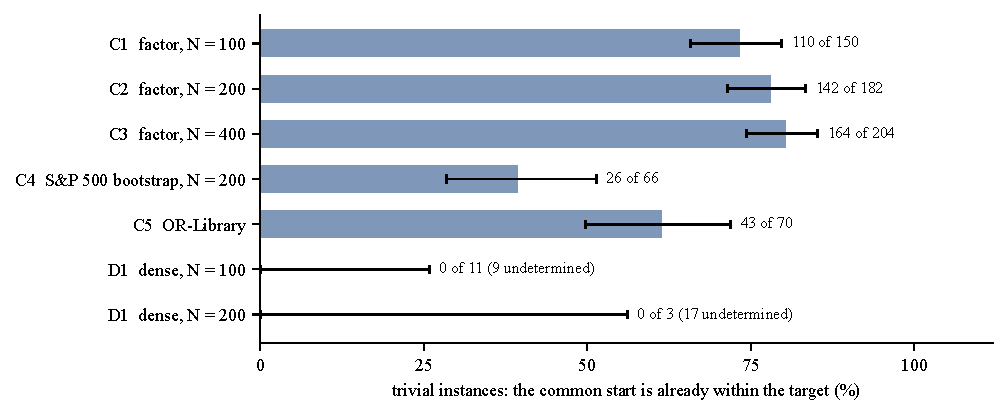
\includegraphics[width=\textwidth]{generated/figures/fig_a3_trivial.pdf}
\caption{Share of trivial test instances by cell: the common start is already within the target
($\hat g \le 10^{-3}$), among the instances the screening decided. Wilson \res{e2.a3.level.pct}\% intervals and
counts; C4 and D1 (dense covariance) are descriptive, and the dense instances the screening left undetermined are
counted apart.}\label{fig:a3}
\end{figure}

\subsection{RQ2: anytime comparison on the non-trivial instances}\label{sec:res-rq2}

The representative of the QUBO class is the tuned winner of the pre-registered tuning, swap-SA, which keeps $K$ assets
by construction and needs no penalty; the penalty samplers of the same runs are reported below. References are
certified optima for all non-trivial instances except \res{e2.c5.uncertified} OR-Library points and the
\res{e2.d1.uncertified} dense ones, where they are the best known values.

\paragraph{Primal integral} Against the open-source exact class, the QUBO pipeline approaches the optimum faster (H2:
pooled $R = \res{e2.h2}$, \res{e2.level.pct}\% CI \res{e2.h2.ci.low}--\res{e2.h2.ci.high}, outcome ``QUBO
better''). The outcome holds without the OR-Library cell (\res{e2.h2.noc5},
\res{e2.h2.noc5.ci.low}--\res{e2.h2.noc5.ci.high}) and when the integral of a method counts from its first
improvement of the common start (\res{e2.h2.firstimpr}); with the integral over $[0, T]$, the measure before the
deviation A2, only its direction is established (\res{e2.h2.full}, \res{e2.h2.full.ci.low}--\res{e2.h2.full.ci.high};
Table~\ref{tab:rq2}). By cell, the advantage is established in C2 and C3, all three OR-Library ports lie on the same
side, and in C1 the data do not distinguish the methods. The comparison is with open-source exact methods only
(Table~\ref{tab:m11}).

Against local search the pooled order is reversed (H2b: $R_b = \res{e2.h2b}$,
\res{e2.h2b.ci.low}--\res{e2.h2b.ci.high}, outcome ``QUBO worse''). This outcome rests on the OR-Library cell, which
has only \res{e2.c5.nports} port clusters, so that its interval is the range of the port means. Without C5 (a post hoc
check) the estimate is \res{e2.h2b.noc5} (\res{e2.h2b.noc5.ci.low}--\res{e2.h2b.noc5.ci.high}), from the first
improvement \res{e2.h2b.firstimpr} (\res{e2.h2b.firstimpr.ci.low}--\res{e2.h2b.firstimpr.ci.high}) and over $[0, T]$
\res{e2.h2b.full} (\res{e2.h2b.full.ci.low}--\res{e2.h2b.full.ci.high}): in each of these variants local search is
faster on average, but the size of the difference relative to the band $[1/1.5, 1.5]$ is not determined. % num-ok: the equivalence band of the plan

The average hides a split over the instances (Table~\ref{tab:rq2-inst}, descriptive and post hoc). On the typical
factor instance the QUBO pipeline is the faster of the two: the median $R_b$ is \res{e2.inst.c1.rb.median},
\res{e2.inst.c2.rb.median} and \res{e2.inst.c3.rb.median} in C1--C3, and $R_b < 1$ on
\res{e2.inst.c1.rb.below.pct}\%, \res{e2.inst.c2.rb.below.pct}\% and \res{e2.inst.c3.rb.below.pct}\% of the
instances. On a minority it fails: the median over its seeds of the time to the target lies beyond the budget on
\res{e2.censor.c1.qubo}, \res{e2.censor.c2.qubo} and \res{e2.censor.c3.qubo} of the 40 instances of C1--C3 and on
\res{e2.censor.c4.qubo} of 40 in C4, and the largest $R_b$ in C1 is \res{e2.inst.c1.rb.max}. The median time to the
target of local search was within the budget on every instance. The geometric mean of the plan weighs these failures, and they decide H2b; on the S\&P and
OR-Library cells local search is also faster on the typical instance (median $R_b$ \res{e2.inst.c4.rb.median} and
\res{e2.inst.c5.rb.median}).

\begin{table}[t]
\centering\small\setlength{\tabcolsep}{4pt}
\caption{RQ2: ratios of the primal integral after the common start, $R = \mathrm{PI}^{+}(\text{QUBO}) /
\mathrm{PI}^{+}(\text{exact})$ and $R_b = \mathrm{PI}^{+}(\text{QUBO}) / \mathrm{PI}^{+}(\text{local search})$; below 1
the QUBO pipeline is better. Cells: estimate and \res{e2.celllevel.pct}\% interval per cell (Bonferroni, simultaneous
99\% over the four pooled cells; for C5 the range of the three port means); $n$ non-trivial instances % num-ok: family level of the plan
(clusters). Pooled rows: \res{e2.level.pct}\% intervals; the last two (post hoc) replace the exact representative by SCIP
with aggressive primal heuristics or by outer approximation in every cell. $^{\dagger}$Descriptive cell, not
pooled.}\label{tab:rq2}
% generated by scripts/paper_tables.py; do not edit by hand.
\begin{tabular}{lrll}
\toprule
Cell & $n$ & $R$ (H2) & $R_b$ (H2b) \\
\midrule
C1 & 40 & 0.447 [0.133, 1.77] & 2.87 [0.864, 11.3] \\
C2 & 40 & 0.0814 [0.0342, 0.229] & 1.47 [0.571, 4.22] \\
C3 & 40 & 0.182 [0.0745, 0.421] & 1.49 [0.712, 3.50] \\
C4$^{\dagger}$ & 40 & 0.723 [0.231, 2.05] & 19.5 [6.28, 54.6] \\
C5 & 27 (3) & 0.109 [0.0292, 0.514] & 7.50 [2.05, 37.1] \\
D1, $N=100$$^{\dagger}$ & 11 & 0.128 [0.0624, 0.304] & 4.15 [1.44, 10.7] \\
D1, $N=200$$^{\dagger}$ & 3 & 0.815 [0.718, 1.000] & 7.28 [4.91, 9.73] \\
\midrule
\multicolumn{2}{l}{Pooled (C1--C3, C5)} & 0.164 [0.106, 0.257] & 2.62 [1.71, 4.08] \\
\midrule
\multicolumn{2}{l}{Without C5 (post hoc)} & 0.188 [0.127, 0.283] & 1.85 [1.26, 2.76] \\
\multicolumn{2}{l}{$\gamma = 1$ until the first improvement} & 0.106 [0.0700, 0.163] & 2.29 [1.42, 3.82] \\
\multicolumn{2}{l}{No common start (cold runs)} & 0.0376 [0.0315, 0.0433] & 0.143 [0.128, 0.167] \\
\multicolumn{2}{l}{PI over $[0, T]$ (with $t_0$)} & 0.738 [0.630, 0.860] & 1.60 [1.34, 2.04] \\
\multicolumn{2}{l}{Exact: SCIP, aggressive heuristics} & 0.108 [0.0703, 0.169] & 2.62 [1.71, 4.08] \\
\multicolumn{2}{l}{Exact: OA in every cell} & 0.128 [0.0783, 0.212] & 2.62 [1.71, 4.08] \\
\bottomrule
\end{tabular}

\end{table}

\begin{table}[t]
\centering\small\setlength{\tabcolsep}{3.5pt}
\caption{RQ2 over the instances (descriptive, post hoc): medians of $R$ and $R_b$, the shares of instances with
ratios below 1, the largest $R_b$, and the instances on which the median time to the target of a method lies beyond
the 60~s budget (target not reached). $^{\dagger}$Descriptive cell.}\label{tab:rq2-inst}
% generated by scripts/paper_tables.py; do not edit by hand.
\begin{tabular}{lrrrrrrrrr}
\toprule
 & & \multicolumn{2}{c}{$R$} & \multicolumn{3}{c}{$R_b$} & \multicolumn{3}{c}{target not reached} \\
\cmidrule(lr){3-4}\cmidrule(lr){5-7}\cmidrule(lr){8-10}
Cell & $n$ & median & $<1$ (\%) & median & $<1$ (\%) & max & QUBO & LS & exact \\
\midrule
C1 & 40 & 0.12 & 62 & 0.79 & 57 & 378 & 6 & 0 & 0 \\
C2 & 40 & 0.026 & 80 & 0.47 & 68 & 81 & 2 & 0 & 0 \\
C3 & 40 & 0.19 & 82 & 0.66 & 57 & 100 & 4 & 0 & 6 \\
C4$^{\dagger}$ & 40 & 2.4 & 38 & 73 & 25 & 249 & 24 & 0 & 0 \\
C5 & 27 & 0.23 & 78 & 10.0 & 22 & 293 & 6 & 0 & 9 \\
D1, $N=100$$^{\dagger}$ & 11 & 0.100 & 100 & 4.0 & 18 & 19 & 1 & 0 & 3 \\
D1, $N=200$$^{\dagger}$ & 3 & 0.75 & 100 & 8.1 & 0 & 9.7 & 3 & 0 & 3 \\
\bottomrule
\end{tabular}

\end{table}

\paragraph{Penalty samplers} With the tuned penalty samplers of the same runs in the place of the representative
(post hoc, Table~\ref{tab:samplers}), the QUBO pipeline is slower than the open-source exact class --- single-flip
annealing $R = \res{e2.sa.h2}$ (\res{e2.sa.h2.ci.low}--\res{e2.sa.h2.ci.high}), tabu search $R = \res{e2.tabu.h2}$
(\res{e2.tabu.h2.ci.low}--\res{e2.tabu.h2.ci.high}) --- and far slower than local search ($R_b = \res{e2.sa.h2b}$ and
\res{e2.tabu.h2b}). In this benchmark the advantage of H2 belongs to the sampler that preserves the cardinality, not to
the penalty samplers.

\begin{table}[t]
\centering\footnotesize\setlength{\tabcolsep}{3pt}
\caption{RQ2 with other QUBO samplers (post hoc): the same estimator with the tuned single-flip annealing (SA) and tabu
search of the same runs, both on the penalty QUBO, in the place of the representative swap-SA; cell estimates and the
pooled estimates over C1--C3 and C5 with \res{e2.level.pct}\% intervals. $^{\dagger}$Descriptive cell.}\label{tab:samplers}
% generated by scripts/paper_tables.py; do not edit by hand.
\begin{tabular}{lllllll}
\toprule
 & \multicolumn{3}{c}{$R$ (against the exact class)} & \multicolumn{3}{c}{$R_b$ (against local search)} \\
\cmidrule(lr){2-4}\cmidrule(lr){5-7}
Cell & swap-SA & SA & tabu & swap-SA & SA & tabu \\
\midrule
C1 & 0.447 & 37.3 & 14.5 & 2.87 & 240 & 93.2 \\
C2 & 0.0814 & 6.06 & 1.55 & 1.47 & 109 & 28.0 \\
C3 & 0.182 & 5.28 & 1.62 & 1.49 & 43.3 & 13.3 \\
C4$^{\dagger}$ & 0.723 & 5.22 & 3.77 & 19.5 & 141 & 102 \\
C5 & 0.109 & 3.02 & 3.02 & 7.50 & 207 & 207 \\
\midrule
Pooled & 0.164 & 7.74 & 3.24 & 2.62 & 124 & 51.7 \\
95\% CI & [0.106, 0.257] & [6.81, 8.79] & [2.56, 4.04] & [1.71, 4.08] & [116, 132] & [41.4, 64.1] \\
\bottomrule
\end{tabular}

\end{table}

\paragraph{The common start decides the order of H2b} Without the common start (cold runs, a sensitivity of the plan)
the order of H2b reverses: $R_b = \res{e2.h2b.own}$ (\res{e2.h2b.own.ci.low}--\res{e2.h2b.own.ci.high}). The reason is
the time to a method's first own portfolio (Table~\ref{tab:exact}): the QUBO pipeline holds one after its first batch
(medians from \res{e2.delay.c1.qubo.median}~s in C1 to \res{e2.delay.c3.qubo.median}~s in C3), local search only when
its greedy construction ends (\res{e2.delay.c1.ls.median}~s to \res{e2.delay.c3.ls.median}~s), and the exact
representative after \res{e2.delay.c1.exact.median}~s to \res{e2.delay.c3.exact.median}~s. The common start itself
is ready earlier still (medians from \res{e2.t0.c1.median}~s in C1 to \res{e2.t0.c3.median}~s in C3), and in the
cold runs no method held its first portfolio before that time on any instance (post hoc). The first portfolio of the
QUBO pipeline was at least as good as the common start on \res{e2.first.c1.qubo.notworse.pct}\%,
\res{e2.first.c2.qubo.notworse.pct}\% and \res{e2.first.c3.qubo.notworse.pct}\% of the instances of C1--C3, that of
local search on \res{e2.first.c1.ls.notworse.pct}\%, \res{e2.first.c2.ls.notworse.pct}\% and
\res{e2.first.c3.ls.notworse.pct}\%. With the common start, the start covers this interval for every method.

\begin{table}[t]
\centering\small
\caption{The exact class by cell (secondary): the exact representative, the median time of its last improvement
$t_{\mathrm{primal}}$ and the share of its runs certified within the 60~s budget; and the median delay to the first
own solution of each representative in the cold runs (no common start). $^{\dagger}$Descriptive cell.}\label{tab:exact}
% generated by scripts/paper_tables.py; do not edit by hand.
\begin{tabular}{llrrrrr}
\toprule
Cell & exact method & $t_{\mathrm{primal}}$ (s) & certified (\%) & \multicolumn{3}{c}{first own solution (s)} \\
\cmidrule(lr){5-7}
 & & & & QUBO & LS & exact \\
\midrule
C1 & SCIP & 1.5 & 100 & 0.064 & 0.59 & 0.55 \\
C2 & SCIP & 8.6 & 72 & 0.19 & 1.6 & 3.9 \\
C3 & OA (HiGHS) & 7.5 & 18 & 0.57 & 3.7 & 7.4 \\
C4$^{\dagger}$ & SCIP & 12 & 68 & 0.19 & 1.2 & 3.9 \\
C5 & SCIP & 15 & 7 & 0.067 & 0.79 & 0.50 \\
\bottomrule
\end{tabular}

\end{table}

\paragraph{Time to target} The time to the target gives the same pooled outcomes (secondary): QUBO over exact
\res{e2.ttt} (\res{e2.ttt.ci.low}--\res{e2.ttt.ci.high}) and QUBO over local search \res{e2.tttb}
(\res{e2.tttb.ci.low}--\res{e2.tttb.ci.high}); re-censored at 10~s, the second weakens to a direction
(\res{e2.tttb.budget10}, \res{e2.tttb.budget10.ci.low}--\res{e2.tttb.budget10.ci.high}). By the performance profiles
at ratio 1~\cite{dolan2002benchmarking}, the QUBO pipeline has the smallest integral on \res{e2.profile.pi.c1.qubo.pct}\%,
\res{e2.profile.pi.c2.qubo.pct}\% and \res{e2.profile.pi.c3.qubo.pct}\% of the instances of C1, C2 and C3, local search
on \res{e2.profile.pi.c4.ls.pct}\% and \res{e2.profile.pi.c5.ls.pct}\% of C4 and C5. The exact representative
certifies the optimum within the budget in \res{e2.exact.c1.cert.pct}\% of its runs in C1, \res{e2.exact.c2.cert.pct}\%
in C2, \res{e2.exact.c3.cert.pct}\% in C3 and \res{e2.exact.c5.cert.pct}\% in C5.

The time-to-target curves~\cite{aiex2006ttt} on three calibration instances of $N = 200$ (100 runs per method,
Figure~\ref{fig:ttt}, descriptive) illustrate the split. Local search reaches the target in every run on all three
instances (medians \res{e2.curves.1014.ls.median}, \res{e2.curves.1043.ls.median} and
\res{e2.curves.1049.ls.median}~s), the exact representative in \res{e2.curves.1014.exact.pct}\%,
\res{e2.curves.1043.exact.pct}\% and \res{e2.curves.1049.exact.pct}\% of its runs (medians
\res{e2.curves.1014.exact.median}, \res{e2.curves.1043.exact.median} and \res{e2.curves.1049.exact.median}~s). The QUBO
pipeline is the fastest method on the first instance (median \res{e2.curves.1014.qubo.median}~s), behind local search
on the second (\res{e2.curves.1043.qubo.median}~s), and never reaches the target within 60~s on the third
(\res{e2.curves.1049.qubo.pct}\% of the runs). These instances were also used for tuning; the counts of
Table~\ref{tab:rq2-inst} come from the test instances.

\begin{figure}[t]
\centering
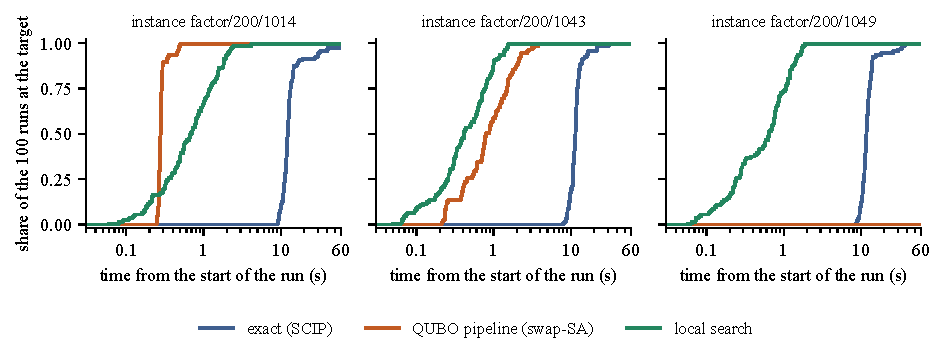
\includegraphics[width=\textwidth]{generated/figures/fig_ttt_curves.pdf}
\caption{Time-to-target curves ($\hat g \le 10^{-3}$) of the three representatives on three calibration instances of
$N = 200$: the share of 100 runs at the target against the time from the start of the run (log scale). Runs that miss
the target stay in the denominator.}\label{fig:ttt}
\end{figure}

\paragraph{The exact baseline}\label{sec:res-m11} The representative of the exact class was chosen by the tuning
criterion, the median $\mathrm{PI}^{+}$ on the calibration instances. At $N = 200$ outer approximation won the 10~s
screen (\res{e2.tune.n200.oa.screen} against \res{e2.tune.n200.scip.screen} for SCIP) but lost the 60~s recheck
(\res{e2.tune.n200.oa.long} against \res{e2.tune.n200.scip.long}), so SCIP is the representative at $N = 100$ and 200
and outer approximation at $N = 400$. On problem~(34) of Bertsimas and Cory-Wright~\cite{bertsimas2022scalable} and
the times of their Tables~3 and~4 (arXiv version~5; BCW-T3 and BCW-T4 below), SCIP needed in the median
\res{e2.m11.t3.scip.median} times the best published time on BCW-T3 and \res{e2.m11.t4.scip.median} times on BCW-T4
(Table~\ref{tab:m11}, Figure~\ref{fig:m11}); outer approximation needed \res{e2.m11.t3.oa.median} times on BCW-T3.
The best published times on BCW-T3 are a few hundredths of a second (median \res{e2.m11.t3.pub.time.median}~s,
printed to two decimals), against a median of \res{e2.m11.t3.scip.time.median}~s for SCIP, including the build of
the model in Python. On BCW-T4 SCIP solved all \res{e2.m11.t4.scip.ncells} instances within the limit, the best
published method \res{e2.m11.t4.scip.npub}, and SCIP was faster on \res{e2.m11.t4.scip.nfaster} of them
(\res{e2.m11.t4.scip.faster.cells}). The times are not normalised for the hardware, and the validation measures the
time to a certificate, not the speed of improvement that H2 measures. By the rule of the plan (a median ratio above
10), the conclusions of RQ2 concern open-source exact methods, and the outcome of H2 carries this caveat.

Two post hoc runs re-solved the same non-trivial instances with other open-source exact baselines (\ref{app:deviations},
19 October; Table~\ref{tab:rq2}): SCIP in the configuration of the representative with its aggressive primal
heuristics, and outer approximation as the representative in every cell. The pooled ratio stays below the band in
both, $R = \res{e2.exactsens.scipaggr.h2}$ (\res{e2.exactsens.scipaggr.h2.ci.low}--\res{e2.exactsens.scipaggr.h2.ci.high})
and $R = \res{e2.exactsens.oa.h2}$ (\res{e2.exactsens.oa.h2.ci.low}--\res{e2.exactsens.oa.h2.ci.high}), so the outcome
of H2 does not depend on these choices of the open-source baseline. The aggressive heuristics did not make SCIP improve
its incumbent faster on the factor and S\&P cells: the median ratio of its primal integral to that of the default
setting was \res{e2.exactsens.scipaggr.pirel.c1} in C1, \res{e2.exactsens.scipaggr.pirel.c2} in C2 and
\res{e2.exactsens.scipaggr.pirel.c4} in C4, against \res{e2.exactsens.scipaggr.pirel.c5} on the OR-Library points.

\begin{table}[t]
\centering\small\setlength{\tabcolsep}{4pt}
\caption{Validation of the exact stack against Tables~3 ($\kappa = 1$, limit 300~s) and~4 ($\kappa = 0$ with a
minimum return, limit 3600~s) of Bertsimas and Cory-Wright (BCW-T3, BCW-T4): the median over the 15 instances of each
table of our time over the best published time (SCIP gives the verdict; outer approximation and the better of our
two methods for reference), the median times, and the instances solved within the limit.}\label{tab:m11}
% generated by scripts/paper_tables.py; do not edit by hand.
\begin{tabular}{lrrrrrrr}
\toprule
 & \multicolumn{3}{c}{median ratio} & \multicolumn{2}{c}{median time (s)} & \multicolumn{2}{c}{solved} \\
\cmidrule(lr){2-4}\cmidrule(lr){5-6}\cmidrule(lr){7-8}
BCW table & SCIP & OA & best of ours & SCIP & BCW best & ours & BCW \\
\midrule
BCW-T3 & 262 & 3.1 & 3.1 & 4.9 & 0.020 & 15/15 & 15/15 \\
BCW-T4 & 14 & -- & 14 & 651 & 21 & 15/15 & 14/15 \\
\bottomrule
\end{tabular}

\end{table}

\begin{figure}[t]
\centering
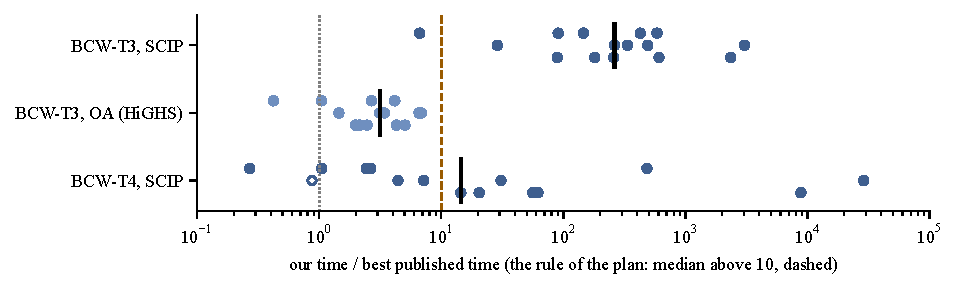
\includegraphics[width=\textwidth]{generated/figures/fig_m11_ratios.pdf}
\caption{Ratio of our time to the best published time per instance (dots, three cardinalities per port) and their
median (bar). Hollow: every published method hit the limit, so the ratio is an upper bound.}\label{fig:m11}
\end{figure}

\subsection{RQ3: does optimisation accuracy matter out of sample?}\label{sec:res-rq3}

On FF49 the cardinality constraint binds on \res{e3.ff.binding.pct}\% of the walk-forward folds (median
$K = \res{e3.ff.k.median}$), and the lower bound of the rule for $K$ is active on \res{e3.ff.regime.lb.pct}\% of them
(\res{e3.us.regime.lb.pct}\% on the US universe): with $K u$ close to one, the weights are nearly fixed and the
alternatives differ mainly in which assets (on FF49, industries) they hold. The best non-optimal support (rank 2) is close to the
optimum in sample: its gap has a median of \res{e3.ff.mv.dose2.median}~bp of certainty equivalent per year for the
mean--variance arm, \res{e3.ff.gmv.dose2.median}~bp for the minimum-variance arm and \res{e3.us.mv.dose2.median}~bp on
the US universe (Table~\ref{tab:rq3-extra}).

For the minimum-variance arm, the rank-2 portfolio and the optimum are equivalent out of sample: the log variance
ratio is \res{e3.ff.gmv.h3a} (\res{e3.h3a.level.pct}\% CI \res{e3.ff.gmv.h3a.ci.low}--\res{e3.ff.gmv.h3a.ci.high})
inside its margin (Holm-adjusted $p_{\mathrm{TOST}} = \res{e3.ff.gmv.h3a.p.tost.holm}$). For the mean--variance arm
(primary) the difference of Sharpe ratios before costs is \res{e3.ff.mv.h3a}
(\res{e3.ff.mv.h3a.ci.low}--\res{e3.ff.mv.h3a.ci.high}) against the margin $\pm\res{e3.ff.mv.margin.high}$:
inconclusive, which is uncertainty and not evidence that accuracy matters. On the US universe the result is also
inconclusive (\res{e3.us.mv.h3a}, \res{e3.us.mv.h3a.ci.low}--\res{e3.us.mv.h3a.ci.high}; Table~\ref{tab:rq3}). These
statements concern the best alternatives, which are close to the optimum by construction, not an error of the same size
in an arbitrary direction.

The sensitivities of the plan leave these outcomes in place: with block lengths of 21 and 63 days instead of the
calibrated ones (\res{e3.ff.mv.block}, \res{e3.ff.gmv.block} and \res{e3.us.mv.block} days) and with execution one day
later the outcomes do not change, nor do they on the US universe with terminal returns of $-30\%$ and $-100\%$ for % num-ok: sensitivity levels of the plan
delisted stocks or on the \res{e3.us.mv.sens.coverage.nfolds} folds on which at least 90\% of the index members have % num-ok: coverage threshold of the plan
usable prices; with the wider margin $\Delta_{\mathrm{SR}} = 0.05$ the mean--variance arm on FF49 % num-ok: sensitivity margin of the plan
becomes equivalent ($p_{\mathrm{TOST}} = \res{e3.ff.mv.sens.dsr005.p.tost}$), on the US universe it does not
($p_{\mathrm{TOST}} = \res{e3.us.mv.sens.dsr005.p.tost}$). After costs of 10~bp per unit of traded notional, the % num-ok: cost level of the plan
difference of Sharpe ratios of the rank-2 path is \res{e3.ff.mv.net10}
(\res{e3.ff.mv.net10.ci.low}--\res{e3.ff.mv.net10.ci.high}) for the mean--variance arm on FF49
(Table~\ref{tab:rq3-extra}).

Along the series of the best alternative supports (H3b, Figure~\ref{fig:dose}), no relation between the in-sample
gap and the out-of-sample Sharpe ratio before costs is detected at this power for the mean--variance arm (slope
\res{e3.ff.mv.h3b.slope} per unit of the logarithm of the dose, \res{e3.h3b.level.pct}\% CI
\res{e3.ff.mv.h3b.slope.ci.low}--\res{e3.ff.mv.h3b.slope.ci.high}); the pointwise interval of the path of rank 5
excludes zero (\res{e3.ff.mv.rank5}, \res{e3.ff.mv.rank5.ci.low}--\res{e3.ff.mv.rank5.ci.high}), one of six
unadjusted intervals. For the minimum-variance arm the relation is significant: a doubling of the mean in-sample dose
raises the out-of-sample variance by \res{e3.ff.gmv.h3b.doubling.pct}\%
(\res{e3.ff.gmv.h3b.doubling.pct.ci.low}--\res{e3.ff.gmv.h3b.doubling.pct.ci.high}\%). H3c is descriptive:
\res{e3.ff.mv.h3c.nmaterial} of the \res{e3.ff.mv.h3c.nsolvers} real solvers leave a material in-sample gap on FF49,
so their calibration against the curve was not tested.

\begin{table}[t]
\centering\footnotesize\setlength{\tabcolsep}{3pt}
\caption{RQ3, H3a (FF49 primary, US secondary): the rank-2 path against the optimum out of sample, as the
difference of Sharpe ratios before costs (MV) or the log variance ratio (GMV); TOST with \res{e3.h3a.level.pct}\%
intervals and the equivalence margins of the plan; $^{*}$Holm-adjusted. $^{\ddagger}$Without the days with irregular
adjustments (sensitivity).}\label{tab:rq3}
% generated by scripts/paper_tables.py; do not edit by hand.
\begin{tabular}{lllll}
\toprule
Market, arm & estimate [90\% CI] & margin & $p_{\mathrm{TOST}}$ & outcome \\
\midrule
FF49, MV & 0.00364 [\ensuremath{-}0.0286, 0.0359] & $\pm$0.0208 & 0.19 & inconclusive \\
FF49, GMV & \ensuremath{-}0.000762 [\ensuremath{-}0.0137, 0.0122] & [\ensuremath{-}0.0417, 0.0400] & \ensuremath{2.0\times10^{-4}}$^{*}$ & equivalent \\
US, MV & \ensuremath{-}0.0183 [\ensuremath{-}0.0765, 0.0399] & $\pm$0.0208 & 0.47$^{*}$ & inconclusive \\
US, MV$^{\ddagger}$ & \ensuremath{-}0.0486 [\ensuremath{-}0.112, 0.0143] & $\pm$0.0208 & 1.0 & inconclusive \\
\bottomrule
\end{tabular}

\end{table}

\begin{table}[t]
\centering\footnotesize\setlength{\tabcolsep}{2.5pt}
\caption{RQ3, the context of H3a: the in-sample gap of the rank-2 path (bp of certainty equivalent per year, median and
interquartile range over the folds) and the difference of Sharpe ratios of the rank-2 path against the optimum after
costs of 10~bp (main) and 30~bp per unit of traded notional, with 95\% intervals.}\label{tab:rq3-extra} % num-ok: cost levels and confidence level of the plan
% generated by scripts/paper_tables.py; do not edit by hand.
\begin{tabular}{llll}
\toprule
Market, arm & dose of rank 2 (bp) & \multicolumn{2}{c}{$\Delta$Sharpe after costs [95\% CI]} \\
\cmidrule(lr){3-4}
 & median [IQR] & 10~bp & 30~bp \\
\midrule
FF49, MV & 6.1 [2.3, 13] & \ensuremath{-}0.0020 [\ensuremath{-}0.041, 0.037] & \ensuremath{-}0.013 [\ensuremath{-}0.052, 0.025] \\
FF49, GMV & 3.3 [1.5, 6.7] & 0.032 [\ensuremath{-}0.013, 0.076] & 0.020 [\ensuremath{-}0.026, 0.064] \\
US, MV & 2.7 [0.93, 7.2] & \ensuremath{-}0.021 [\ensuremath{-}0.092, 0.049] & \ensuremath{-}0.025 [\ensuremath{-}0.097, 0.046] \\
\bottomrule
\end{tabular}

\end{table}

\begin{figure}[t]
\centering
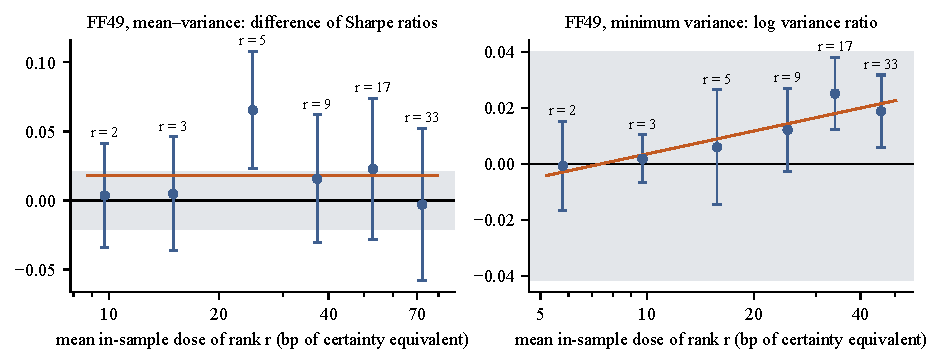
\includegraphics[width=\textwidth]{generated/figures/fig_rq3_dose.pdf}
\caption{FF49: the out-of-sample difference of the path that holds the support of rank $r$ against the optimum, by its
mean in-sample dose, with pointwise \res{e3.h3b.level.pct}\% intervals, the fitted H3b line and the equivalence margin
(grey).}\label{fig:dose}
\end{figure}

% sections/discussion.tex — numbers only through \res{}; every claim has a row in paper/CLAIMS.md.
% Draft for the author's review (plan of sections approved 2026-10-18, PLAN §6); revised after the review r1.
\section{Discussion}\label{sec:discussion}

\subsection{When does a QUBO pipeline pay?}\label{sec:disc-when}

The answer depends on the instance, on the sampler and on what a method starts from. With a cheap classical start ---
the continuous relaxation rounded to its $K$ largest weights and refined --- most of our factor and OR-Library
instances and a substantial share of the S\&P instances need no combinatorial search at all, and on the factor
instances the gaps that remain are a few basis points of certainty equivalent per year (Section~\ref{sec:res-a3}).
On the remaining instances, a pipeline whose sampler preserves the cardinality approached the optimum faster than the
open-source exact solvers, while the pipelines with the tuned penalty samplers did not (Section~\ref{sec:res-rq2}).
Against a local search on the true objective, the pipeline was faster on the typical factor instance but failed to
reach the target within the budget on a minority of them and on most of the S\&P instances; local search never
failed, and on average it was faster (the direction of H2b is established, its size relative to the band is not).
The pipeline therefore offers speed on many instances without reliability, and local search offers both on average.

A niche for a fast first portfolio is not supported either. Without the common start the pipeline holds its first
portfolio sooner than local search and the exact methods, which reverses the order of H2b (Table~\ref{tab:exact}), but
the common start itself is ready earlier on every instance, and the first portfolio of the pipeline is at least as
good as it on most, but not all, instances. For the CCMV problem, where the continuous relaxation is always available and cheap, a QUBO pipeline
did not deliver a portfolio sooner than the classical start.

The results of RQ1 suggest a mechanism, which we did not test at the sizes of RQ2. At $N \le 24$ the ceiling of the
equal-weight surrogate rises with the dispersion of volatilities, an oracle pool of the best subsets of the surrogate
recovers most of the loss, and the real samplers either miss the minimum of the surrogate (penalty annealing) or
find it but return few distinct subsets per call (tabu search and swap-SA), so that their pools recover less of the
loss than the oracle pool (Table~\ref{tab:samplers-rq1}). A pipeline that ranks subsets by the surrogate inherits its
ceiling unless its pool is diverse; local search ranks supports by the true objective at every step.

These findings bear on how QUBO approaches to portfolio selection are usually evaluated. Positive results in the
literature rest mostly on closed hybrid services and on weak or untuned classical
baselines~\cite{mugel2022dynamic,lang2022strategic,kim2025quantum}, while strong classical solvers, where they are
present, solve the portfolio problems considered~\cite{lozano2026where,stopfer2025quantum,chen2025benchmarking}. Our
benchmark differs from these studies in three respects: an anytime measure under equal budgets and one tuning
protocol for all methods~\cite{barr1995designing,bucher2024towards}, a local search on the true objective as a
classical baseline of the same kind as the pipeline, and a screening of trivial instances. On the calibration
instances the common start was already within the target on most instances, so without the screening the outcome
``equivalent'' could have been fixed by the composition of the cells rather than by the methods.

\subsection{What the exact baseline means for H2}\label{sec:disc-baseline}

On the problems of Bertsimas and Cory-Wright~\cite{bertsimas2022scalable}, our open-source exact representative was more
than an order of magnitude slower than the best published methods, while outer approximation with an open-source master
problem stayed within an order of magnitude on BCW-T3, and on the hardest instances of BCW-T4 SCIP was competitive
(Section~\ref{sec:res-m11}). The validation measures the time to a certificate, and H2 measures the speed of improving
an incumbent; the two need not agree, and the representative was chosen on the second. Its tuning space was small
--- the formulation and the symmetry handling, \res{e2.tune.exact.n100.nconfigs} and \res{e2.tune.exact.n200.nconfigs}
configurations searched completely, against \res{e2.tune.heur.nconfigs} random configurations of each heuristic.
Two post hoc runs probed this choice: with SCIP's aggressive primal heuristics, and with outer approximation as the
representative in every cell, the outcome of H2 was unchanged, and the aggressive heuristics did not speed up the
improvement of SCIP's incumbent (Section~\ref{sec:res-m11}). H2 therefore states that the QUBO pipeline with a
cardinality-preserving sampler outpaces open-source exact solvers, which matters where commercial solvers are not
available; it does not state that the pipeline outpaces the best exact methods. Studies that include
strong commercial solvers find them solving their portfolio problems quickly, but those problems differ from ours (a
binary surrogate, or no cardinality constraint)~\cite{lozano2026where,stopfer2025quantum}; whether H2 would hold against
such solvers is not tested here.

\subsection{Does optimisation accuracy matter out of sample?}\label{sec:disc-oos}

For minimum-variance portfolios, the best non-optimal support is equivalent to the optimum out of sample, and the
out-of-sample variance grows with the in-sample dose along the series of the best alternatives; for mean--variance
portfolios the comparison is inconclusive, and no dose--response is detected at this power
(Section~\ref{sec:res-rq3}). Both statements are about small and specific errors: the best alternatives are a few basis
points of certainty equivalent per year worse than the optimum in sample, and on almost all folds the lower bound of
$K$ holds the weights nearly fixed, so that the alternatives differ mainly in which assets they hold. The difference between the
arms may reflect that the objective of the minimum-variance arm is the variance itself, while the mean--variance
objective also carries the estimated means, whose error is known to dominate out of
sample~\cite{michaud1989markowitz,kan2007optimal,demiguel2009optimal}; with the mean--variance outcome inconclusive,
this is a hypothesis, not a finding. Gilli and Schumann found that beyond some point better solutions of a portfolio
problem do not give better portfolios~\cite{gilli2011optimal,gilli2012heuristic}; constraints and sparsity act as
regularisers~\cite{jagannathan2003risk,brodie2009sparse}. Our design adds certified optima, exactly enumerated
alternatives with measured doses and pre-registered equivalence tests. It confirms equivalence for the minimum-variance
arm and leaves the mean--variance arm open, as the power analysis of the pilot anticipated. On FF49 the real solvers left
almost no in-sample gap, so their own out-of-sample losses could not be calibrated against the curve.

The two parts of the paper meet here. The anytime race of RQ2 on the factor instances is run for start gaps of at
most \res{e2.a3.c2.gstart.max.bp}~bp of certainty equivalent per year, below the smallest effect of interest of RQ3
(25~bp); such in-sample differences between good methods are smaller than the out-of-sample differences that the % num-ok: smallest effect of interest of the plan
mean--variance arm of RQ3 could resolve.

\subsection{Practical guidance}\label{sec:disc-guidance}

For cardinality-constrained mean--variance problems of the sizes studied here, the evidence supports the following
order of work.
\begin{enumerate}
\item Build the common start: solve the continuous relaxation, keep its $K$ largest weights and refine them. It takes a
fraction of a second in the median, and on most of our factor and OR-Library instances it is already within the
target.
\item If a certificate matters, give the start to an exact solver; on the trivial instances the bound closes the
question, at a cost that ranged from seconds at $N = 100$ to more than an hour on some instances
(Section~\ref{sec:res-a3}).
\item To improve on the start, run a local search on the true objective with refinement of the weights; in our
benchmark its median time to the target was within the budget on every instance, and it was the more reliable anytime
method.
\item If a QUBO pipeline is used, for example as the classical counterpart of a quantum sampler, give it a sampler that
preserves the cardinality and a diverse pool: with the penalty samplers of our tuning space it did not improve on
open-source exact solvers (Section~\ref{sec:res-rq2}).
\end{enumerate}

\subsection{Limitations}\label{sec:disc-limits}

The exact baseline is open-source and runs on one thread, its tuning space was small (two post hoc alternatives left
H2 unchanged), and the validation against published times measures certificates and is not normalised for the
hardware; the conclusions of RQ2 are about open-source exact methods. All timings come from one shared
server, with at most 16 pinned single-threaded jobs and the load recorded with each run. The confirmatory cells C1--C3
are synthetic, and their share of trivial instances depends on the design ($K$ half the support of the continuous
optimum, $\lambda = 5$, $\tau = 10^{-3}$); the S\&P cell is descriptive because its pre-registered rule found no
admissible risk aversion, the OR-Library cell has only three port clusters, and the band outcome of H2b depends on it.
References are best known values, not certificates, on \res{e2.n.uncertified} of the \res{e2.n.instances} non-trivial
instances, and most dense instances were left undetermined by the screening. The tuning spaces were frozen before the
pilot: at their penalty levels single-flip annealing could not leave the start, so H1c reads narrowly, and the penalty
samplers were not given smaller penalties; other QUBO samplers, such as parallel tempering or simulated bifurcation,
were not tested. RQ1 is limited to $N \le 24$. The samplers are classical. The ceiling of the surrogate, however, is
the limit that a pipeline with any sampler of the same surrogate approaches as the minimisation improves, quantum
annealers and QAOA included; it is not a bound, since a diverse pool can do better than the exact minimiser of the
surrogate. Out of sample, the primary tests use 49 industry portfolios in a regime of nearly fixed weights; the US
universe is secondary, its calibrated block length was one day, and the power for the mean--variance arm was low.

% sections/conclusion.tex — numbers only through \res{}; every claim has a row in paper/CLAIMS.md.
% Draft for the author's review (plan of sections approved 2026-10-18: the answer to each question in one or two
% sentences); revised after the review r1.
\section{Conclusion}\label{sec:conclusion}

We compared QUBO-based heuristics with open-source exact solvers and with a local search on the true objective for the
cardinality-constrained mean--variance problem, in a benchmark whose hypotheses, metrics and tests were fixed before
the pilot runs.

At $N \le 24$, the equal-weight binary surrogate limits a QUBO pipeline more when the volatilities and betas of the
assets are more dispersed; an oracle pool of its best subsets removes most of this limit, but the real samplers return
few distinct subsets per call, and in the frozen tuning space tabu search improved the common start where single-flip
simulated annealing could not (RQ1). On most factor and OR-Library instances and on a substantial share of the S\&P~500
instances, the refined solution of the continuous relaxation was already within the target, and on the factor instances
the gaps that remained were a few basis points of certainty equivalent per year. On the remaining instances a pipeline
with a cardinality-preserving sampler approached the optimum faster than open-source exact solvers, while pipelines
with penalty samplers did not; against local search it was faster on the typical factor instance but failed on a
minority of instances, and local search was faster on average and, in the median over its runs, reached the target
within the budget on every instance. Since the open-source exact baseline was
much slower than the best published methods, the advantage over exact methods concerns open-source solvers only,
although it held under the two alternative open-source baselines we tried (RQ2).
Out of sample, the best non-optimal support was equivalent to the optimum for minimum-variance portfolios, although the
out-of-sample variance grew with the in-sample gap along the series of alternatives; for mean--variance portfolios the
comparison was inconclusive at the power of the study, which is uncertainty rather than evidence that accuracy matters
(RQ3).

For practice, the evidence supports building the common start first, giving it to an exact solver when a certificate is
needed, and improving it by a local search on the true objective; a QUBO pipeline needs a sampler that preserves the
cardinality and a diverse pool to compete, and even then it was less reliable than local search. The open questions are
those of the limitations: commercial and multi-threaded exact solvers, other QUBO samplers and smaller penalties, and
the same protocol on quantum hardware.

% sections/appendix.tex — the deviations from the pre-registered plan that bear on the results (the full dated log is
% section 12 of the analysis plan in the code archive) and the relation to the earlier study. Draft for the author's
% review; revised after the review r1 (missing entries of the log, entries recorded after the analysis marked); no
% explicit list of corrections of the earlier study (authors' decision 2026-11-04).
\appendix

\section{Deviations from the pre-registered plan}\label{app:deviations}

Table~\ref{tab:deviations} lists the entries of the deviation log that bear on the results, in the order of their
dates (October 2026). Each entry was recorded with its reason before the rows it affects were analysed, except those
marked $^{\ast}$: these were recorded after an audit or a review had seen the affected rows, and they interpret or
correct, but do not change, the estimates.

% a longtable: the log does not fit on one page
{\footnotesize\setlength{\tabcolsep}{3pt}
\begin{longtable}{>{\raggedright\arraybackslash}p{0.07\textwidth}>{\raggedright\arraybackslash}p{0.4\textwidth}>{\raggedright\arraybackslash}p{0.29\textwidth}>{\raggedright\arraybackslash}p{0.17\textwidth}} % num-ok: column widths
\caption{Deviations from the pre-registered plan.}\label{tab:deviations}\\
\toprule
Date & Change & Reason & Affects \\
\midrule
\endfirsthead
\multicolumn{4}{l}{Table~\ref{tab:deviations} (continued)}\\
\toprule
Date & Change & Reason & Affects \\
\midrule
\endhead
\bottomrule
\endlastfoot
11 Oct & Runs on a shared server: at most 16 single-threaded jobs pinned to physical cores, load recorded, instead of
an exclusive machine & no exclusive machine available & timings of RQ2, H1c \\
11 Oct & Public timestamp by an RFC~3161 service instead of an archive deposit & practical & none \\
11 Oct & Methods are compared only on non-trivial instances, decided at the reference stage before any method runs
& on the calibration instances the common start was within the target on most instances; the outcome
``equivalent'' would have been fixed by the composition of the cells & H2, H2b, H1c, tuning \\
11 Oct & Primary measure $\mathrm{PI}^{+}$, the integral after the common start & the common term $t_0/T$ bounds every
ratio & H2, H2b, tuning \\
11 Oct & New estimate: the share of trivial instances per cell (A3) & a direct answer to when solver quality matters &
RQ2 (wording) \\
11 Oct & Sensitivities: the integral from the first improvement of the start and cold runs without the start; the
confined primal integral dropped & the planned variant is not computable from warm runs & H2, H2b (sensitivities) \\
11 Oct & H1c on non-trivial instances; differences below $10^{-8}s$ are zeros & on trivial instances both pipelines sit
at the start or the optimum & H1c \\
11 Oct & RQ1: the work of a tabu call is counted in reads; the residual of the sampler is reported with the size of
its pool and split into precision and the cost of a short pool; reference configurations at $N \le 24$, where nothing
was tuned & one call of a sampler returns few distinct subsets & RQ1 estimates (not H1a, H1c) \\
11 Oct & C4 descriptive (the $\lambda$ rule admitted no value) and run at $\lambda = 20$ & rule of the plan & composition
of the pooled estimate \\
12 Oct & D1 screened on its 40 planned seeds with a 600~s limit & SCIP barely progresses on dense instances & D1 only \\
12 Oct & H1c reads narrowly: in the frozen grid, single-flip annealing is held by the penalty barrier and never improved
the start on calibration & audit of the first checkpoint & H1c (interpretation) \\
12 Oct & The real solvers of RQ3 receive the common start, so the path of annealing in H3c is the path of the start &
comparable solvers at one start & H3c \\
12 Oct & A batch of tabu search in RQ2 has 10 reads, a constant outside the tuning space; one tabu configuration of H1c
was chosen by its number from an exact tie & disclosure (audit of the first checkpoint) & H1c \\
12 Oct & The regime of nearly fixed weights on FF49 ($K u$ close to one) is reported & seen on the pilot & RQ3
(interpretation) \\
12 Oct & Readings of the estimators of H2, H2b and the secondary analyses fixed in code before the bench runs & the
plan left them open & H2, H2b, secondary \\
12 Oct & US sensitivity without irregular adjustment days excludes a stock only from the folds whose windows contain
such a day & the earlier reading selected on a future event & H3a sensitivity \\
17 Oct$^{\ast}$ & A warning and a post-hoc estimate without the cell for pooled cells with fewer than five clusters
(C5) & audit of the confirmatory stages & H2b (interpretation) \\
17 Oct$^{\ast}$ & A certificate of any screening round counts; the analyses were recomputed & a merge of two rounds
lost one certificate; no ratio changed & reference type of one instance \\
17 Oct & Time-to-target curves, the delay to the first own solution and the validation of the exact stack, with their
readings fixed before the rows were read & outputs of the plan not yet reported & secondary analyses of RQ2 \\
17 Oct & The delay of local search is read from its trajectory, not from a field that marked the first refinement of a
partial subset & audit of the confirmatory stages & delay (secondary) \\
18 Oct & The verdict of the validation reads the times of SCIP, the representative at these sizes; recorded before
the run, after exploratory runs outside the registry in which outer approximation was faster & the rule judges the
baseline of H2 & validation of the exact stack \\
18 Oct & The Russian market (exploratory) is left out of this paper & scope of the journal paper & RQ3 (exploratory) \\
19 Oct & Post hoc descriptions: the distribution of $R$ and $R_b$ over the instances$^{\ast}$; the penalty samplers in
the place of the representative; the first own portfolio against the common start (the last two recorded before
they were computed) & review of the manuscript & RQ2 (description) \\
19 Oct & Post hoc sensitivity of H2 to the exact baseline: new runs of SCIP with aggressive primal heuristics (C1--C5)
and of outer approximation (C1, C2, C4, C5) on the same instances, recorded before the runs & review of the
manuscript & RQ2 (sensitivity) \\
\end{longtable}}

\section{Relation to the earlier study}\label{app:prior}

Table~\ref{tab:prior} compares the present design with that of our earlier study of the same
pipeline~\cite{avdoshin2026discrete}. The results of the earlier study are not reused: where the present design answers one of its questions,
the answer comes from the new runs.

% a longtable, so that the table stays in this appendix and does not float behind the references
{\footnotesize\setlength{\tabcolsep}{3pt}
\begin{longtable}{>{\raggedright\arraybackslash}p{0.16\textwidth}>{\raggedright\arraybackslash}p{0.38\textwidth}>{\raggedright\arraybackslash}p{0.38\textwidth}} % num-ok: column widths
\caption{The earlier study and this paper.}\label{tab:prior}\\
\toprule
Aspect & Earlier study & This paper \\
\midrule
\endfirsthead
\multicolumn{3}{l}{Table~\ref{tab:prior} (continued)}\\
\toprule
Aspect & Earlier study & This paper \\
\midrule
\endhead
\bottomrule
\endlastfoot
Sources of the gap & three candidate sources (formulation, sampler, penalty calibration) named, not separated &
the ceiling of the surrogate and the residual of the sampler, against certified optima (RQ1) \\
Instances & synthetic covariance whose volatilities grow with $N$, with near-zero correlations; on the S\&P~500
walk-forward the cardinality constraint did not bind & factor family with a controlled dispersion and a binding $K$ by
construction, S\&P~500 bootstrap, OR-Library; screening of trivial instances \\
Reference & best solution found & certified optimum where SCIP closes the gap, the best known value otherwise, with its
type reported \\
Exact baseline & SCIP and ECOS\_BB through CVXPY, at default settings & native SCIP with the perspective
reformulation and outer approximation, tuned and validated against published times \\
QUBO heuristics & simulated annealing, described as quantum-inspired & simulated annealing, tabu search and swap-SA,
tuned with one protocol and described as QUBO-based heuristics \\
Local search & none & greedy construction and swaps on the true objective \\
Time & median wall time of a run & anytime: primal integral after a common start, time to target, delay to the first
solution \\
Statistics & medians over three seeds, no tests & pre-registered hypotheses, bootstrap intervals, equivalence bands,
Holm's adjustment \\
Out of sample & returns as if rebalanced daily to the target weights, costs once per fold, turnover between target weights,
Sortino ratio from a step equity curve; the heuristic ranked candidates with a turnover cost that the exact solver did
not see & buy-and-hold with drift inside the test window; all paths solve the same problem; exactly enumerated
alternative supports and equivalence tests \\
US universe & the first 100 constituents of the current S\&P~500 list in alphabetical order of company names &
constituents at the formation date, ranked by median dollar volume \\
\end{longtable}}


\section*{Data and code availability}
The code, the configuration files, the registry of runs, the analysis outputs from which every number, table and figure
of this paper is generated, and the frozen analysis plan with its RFC~3161 timestamp are available at
\url{https://github.com/KonstantinPatrushev/qubo-ccmv-benchmark} (code under the MIT licence, results under CC BY 4.0) % num-ok: licence name
and archived on Zenodo, \todo{Zenodo DOI}. The OR-Library problems are public~\cite{beasley1990orlibrary}. The 49 industry
portfolios and their risk-free rate come from the data library of Kenneth
French\footnote{\url{https://mba.tuck.dartmouth.edu/pages/faculty/ken.french/data_library.html}}, and the US
risk-free rate is the series DTB3 of FRED\footnote{\url{https://fred.stlouisfed.org/series/DTB3}}. The membership of
the S\&P~500 was reconstructed from public Wikipedia pages, and prices and volumes were downloaded from Yahoo Finance;
these data are not redistributed, and the archive contains the code that downloads and builds them and the hashes of
the files used.

\section*{CRediT authorship contribution statement}
\textbf{Sergey M. Avdoshin:} Conceptualization, Supervision, Writing -- review \& editing.
\textbf{Konstantin A. Patrushev:} Conceptualization, Methodology, Software, Validation, Formal analysis, Investigation,
Data curation, Writing -- original draft, Visualization.

\section*{Declaration of competing interest}
The authors declare that they have no known competing financial interests or personal relationships that could have
appeared to influence the work reported in this paper.

\section*{Acknowledgements}
% Reporting rules of the HSE supercomputer (hpc.hse.ru/users/report, read 2026-11-04): the required phrase and the
% optional reference to the counter article. The runs of this paper were on another server (Section 4.4); the earlier
% study it builds on was computed in part on the HSE supercomputer (its own acknowledgement), hence the scope.
The supercomputer of HSE University~\cite{kostenetskiy2026high} was used to conduct the computational research of the
earlier study on which this work builds~\cite{avdoshin2026discrete}.

\section*{Funding}
This research did not receive any specific grant from funding agencies in the public, commercial, or not-for-profit
sectors.

\section*{Declaration of generative AI and AI-assisted technologies in the manuscript preparation process}
% Elsevier's template statement (policy page, read 2026-10-19); purposes from docs/AI_USE.md. The second sentence
% becomes true only after the authors' own revision of the drafts — confirm before submission.
During the preparation of this work, the authors used Claude Code (Anthropic) in order to search and screen the
literature, to draft sections of the text from the authors' outline and the registered results, and to check the
consistency of the text with the results and the references. After using this tool, the authors reviewed and edited
the content as needed and take full responsibility for the content of the published article. The use of the same tool
for code and analysis is described in Section~\ref{sec:code}. % accepted by the authors 2026-11-04; true at submission

\bibliographystyle{elsarticle-num}
\bibliography{refs}

\end{document}
